\documentclass[11pt]{article}
\usepackage[utf8]{inputenc}
\usepackage[T1]{fontenc}
\usepackage{amsmath, amsfonts, amssymb, amsthm}
\usepackage[numbers, sort&compress]{natbib}
\usepackage{mathtools}
 \usepackage{tabularx}
\usepackage{geometry}
\geometry{margin=1in}
\usepackage{float}
\usepackage{placeins}   % for \FloatBarrier
\usepackage{caption}    % nicer caption control
\captionsetup[figure]{font=small,labelfont=bf}
\usepackage{enumitem}
\usepackage[hidelinks]{hyperref}
\usepackage{orcidlink}
\usepackage{cleveref}
\usepackage[final]{microtype}
\usepackage{proof} 
\usepackage{csquotes}
\usepackage{booktabs}
\usepackage[most]{tcolorbox}
\usepackage{tocloft}

% Increase space reserved for subsection numbers in TOC:
\setlength{\cftsubsecnumwidth}{2.8em} % default ~2.3em
\setlength{\cftsecnumwidth}{2.8em}      % optional, if sections are also tight


\newtcolorbox{infobox}[1][]{
  enhanced,
  breakable,
  colback=white,
  colframe=black!15,
  fonttitle=\bfseries,
  colbacktitle=black!3,
  coltitle=black,
  % pass through any key–value options from the environment:
  #1,
  boxsep=1ex,
  left=1ex,right=1ex,top=1ex,bottom=1ex,
  before skip=1ex, after skip=1ex
}

% === Theorem environments (uniform upright) ===

\newtheoremstyle{upright}%
  {3pt}{3pt}%   Space above/below
  {\normalfont}% Body font (upright)
  {}%           Indent amount
  {\bfseries}%  Head font
  {.}%          Punctuation after head
  {.5em}%       Space after head
  {}%           Head spec

\theoremstyle{upright}

\newtheorem{theorem}{Theorem}
\newtheorem{assumption}{Assumption}
\newtheorem{example}{Example}
\newtheorem{lemma}{Lemma}
\newtheorem{corollary}{Corollary}
\newtheorem{proposition}{Proposition}
\newtheorem{definition}{Definition}
\newtheorem{remark}{Remark}

\title{Being as a Representable Functor:\\
A Yoneda-Style Ontological Schema Experiment}
\author{Lorand Bruhacs\,\orcidlink{0009-0004-6751-0715}}
\date{\normalsize Preprint, \today \\ DOI \href{https://doi.org/10.5281/zenodo.17441618}{10.5281/zenodo.17441618}}

\begin{document}
\maketitle

\begin{abstract}
\noindent
This paper develops a \emph{critical experiment} that recasts ontological existence schemata in categorical terms. We ask when a functorial “index of ways of being” comes not from many unrelated lists but from a \emph{single universal source}. This yields a two–layer reading: a \emph{cataphatic} layer, where attributes are the natural, lawlike manifestations of the source across contexts; and an \emph{immanent–apophatic} layer, where the source’s reflexive self–structure modulates every manifestation yet resists total capture. We add a disciplined treatment of \emph{omniscience}. Modeled as a modality, it collapses knowledge \emph{extensionally} at a stage (everything true there is “known” and known to be known) but neither produces a single internal statement of global collapse nor an algorithmic method for extracting witnesses to truth. From this, we obtain a \emph{price tag} for realist \emph{self–communication} claims (e.g., ``Jesus is God'' read in–language as an identification of a designated locus with the universal source): internally, such claims require strength beyond purely finitary reasoning, or else call for strong structural assumptions or a richer ambient in which the identification holds by design. The stance is exploratory rather than doctrinal. We do not settle metaphysics; we map formal feasibility, mark theorem–backed limits, and make explicit the extra commitments—computational or structural—by which a regulative horizon is upgraded to constitutive realism.
\end{abstract}

\tableofcontents

\section{Introduction}

\paragraph{Prelude.}
From the earliest myths of a single archê to Plato’s \emph{Good}, Aristotle’s unmoved mover, medieval \emph{ipsum esse}, Spinoza’s substance, and modern structural realisms, philosophy has repeatedly asked whether there is a \emph{universal principle}—a source or pattern by which the many hang together. That question has not grown obsolete; it has changed venues. Today we at last possess formal tools that speak natively about universality, dependence, and limitation: universal properties, representability, descent, and internal logics. This paper proposes that these tools allow us to \emph{re-examine} the ancient inquiry without pretending to settle it: to ask what it would take, \emph{structurally}, for “being” to admit a universal role; how that role weakens depending on the setting; and where principled floors and ceilings may be found. We propose a new vantage—one that lets ancient intuitions and contemporary mathematics meet without talking past each other.

\paragraph{A thought experiment in a \emph{Prolegomena} register.}
This paper is a \emph{critical} exercise rather than a doctrinal metaphysics. In Kant’s sense of a \emph{Prolegomena} \citep{Kant1998}—a preliminary mapping of the conditions under which certain kinds of claims would be possible—we ask: under what explicitly stated categorical hypotheses would there exist an object \(G\) that \emph{represents} a functor of being \(\mathbf B:\mathcal C\to\mathbf{Set}\) (or into a topos), i.e. \(\mathbf B\cong \mathcal C(G,-)\)? The question is structural: it replaces the Anselmian idiom “Does a maximal being exist?”  \citep{Anselm1965} with “When do the formal \emph{conditions} for a universal representing object obtain?” We then examine what follows \emph{within} the model, and where principled limits arise. On our reading, the Kantian critical method does not \emph{ipso facto} forbid application to the question of being (or to any other philosophical question); it only forbids \emph{illicitly} treating Ideas as constitutive of objects beyond possible experience. In this sense, the critical program is not a straightjacket but a \emph{discipline}: it licenses us to map the formal \emph{conditions of representation} and to display the \emph{bounds of reason} within which any ontological reading must operate.

Accordingly, our stance is avowedly \emph{as-if}. We treat “God” as a label for the \emph{representing object} of \(\mathbf B\) where such an object exists, much as Kantian “Ideas of Reason” guide inquiry without constituting objects of possible experience. Nothing here presumes that any chosen \(\mathcal C\) or \(\mathbf B\) uniquely captures reality; rather, the value lies in making the assumptions legible, the inferences transparent, and the limits visible. And while applying formal methods in this register may seem unusual—such tools are often sequestered as “pure mathematics” or applied only to empirical science—\emph{formal methods have no intrinsic domain}: they are a neutral toolkit for analyzing structure wherever structure is claimed, whether in mathematics, science, or metaphysics. Furthermore, there is ample precedent of using category theory for analysis of ontological concepts such as being and becoming (e.g. \citep{Lawvere2005TCS}).

Our posture is not a repudiation of “naïve” or robust metaphysics that argues directly for the existence and attributes of a deity. We simply adopt a different register: one that foregrounds the \emph{conditions of representation} and the \emph{scope} of structural inference. Readers who favor stronger metaphysical commitments are invited to regard our results as diagnostic tools: they indicate which formal features would have to be present in any framework purporting to support such commitments. 

\emph{Methodologically}, we assume a mild, analytic separability of \emph{form} (the structural role of universality, dependence, limitation) from \emph{content} (the substantive doctrinal claims). In traditions where such separability is explicitly rejected—e.g., strong revelational theologies that deny natural theology in principle (Barth’s rejection of the \emph{analogia entis})—our results do not apply; there the conditions for working with formal structure are not met. We do not claim that theology or metaphysics \emph{must} be separable in this way; only that \emph{if and where} they are, the present framework provides a precise language for articulating and testing the structural side of the question.

\paragraph{Interpretive stance.}
Throughout we suggestively \emph{read} $\mathbf B$ as ``being'' and so intentionally tilt the discussion toward an ontological schema; the formalism itself, however, is neutral. One can equally take $\mathbf B(X)$ to classify admissible \emph{descriptions} or \emph{ways of knowing} $X$ (epistemic/cognitive semantics), \emph{observables}/\emph{channels} (information/computation), \emph{models}/\emph{behaviors} of a system (scientific modeling, systems theory), \emph{performances}/\emph{uses} (social/linguistic pragmatics), \emph{valuations}/\emph{interpretations} (logical/semantic metatheory), or \emph{states}/\emph{solutions} (physics/dynamics). In each reading, representability isolates when such admissible modes admit a \emph{universal generator} $G$, while its weakenings (local, pro-/Ind-, stacky, derived) register pluralism, context, symmetry, or deformation. This is a feature, not a defect. The semantic under\-determination of $\mathbf B$ does not dilute the theological thread; it \emph{broadens} it: the same structural argument can be stress-tested across non-theological domains, and its survival there indicates that what is doing the work is a universal-property pattern rather than a domain-specific choice of interpretation. Among non-ontological readings, information geometry is the most literal: taking $\mathbf B(X)$  to be pairs of distributions yields a representer \(G = \Delta_2\), attributes as divergences/metrics, and a transparent endomorphism action---the very same stratification we interpret as cataphatic/apophatic in an ontological-theological reading of $\mathbf B$.

\paragraph{Critical metaphysics, not constitutive ontology.}
By \emph{critical} we mean three things. First, we distinguish \emph{constitutive} from \emph{regulative} uses of structure: representability (\(\mathbf B\cong\mathcal C(G,-)\)) is constitutive \emph{inside} the stipulated model, while its theological reading is merely regulative. Second, we separate \emph{formal results} from \emph{interpretive gloss}. Where possible we prove the former and bracket the latter. Third, we actively police the boundary against \emph{transcendental illusion}: confusing the existence of a representing object in a category with a metaphysical proof \emph{about the world}.

Relative to that method, this paper advances a conditional narrative. If \(\mathcal C\) satisfies standard completeness/smallness assumptions and \(\mathbf B\) satisfies continuity and solution-set conditions, then \(\mathbf B\) is representable. If \(\mathbf B\) is representable, then cataphatic talk about “attributes” is captured by natural transformations out of \(\mathcal C(G,-)\). If the internal logic is sufficiently expressive, then fixed-point and undefinability phenomena impose non-trivial ceilings on any attempt to totalize such attributes. Each “if” wears its assumptions on its sleeve.

Our project here can be read as a Quinean semantic ascent \citep{Quine1960} from first-order metaphysical disputes to a metalanguage of formal structure. Instead of arguing \emph{within} metaphysics about whether a \(G\) is ultimate, we ascend to talk about how different metaphysical theories relate to formal structure. The categorical framework is the metalanguage for that ascent, in which ontologies can be compared without presupposing which one is true. We emphasize \emph{pluralism}. There is no single, privileged choice of \(\mathcal C\) or \(\mathbf B\). Different readings of “being” and “participation” will induce different functors, and thus different existence questions. Our aim is to isolate a portable formal pattern and to show how interpretive choices propagate through it.

\paragraph{Contributions.}
(i) We formulate a \emph{representability-of-being} schema that yields a universal source object \(G\) (unique up to iso) under standard categorical hypotheses. 
(ii) We articulate a \emph{cataphatic layer} in which “attributes” are natural transformations \(\mathcal C(G,-)\Rightarrow \mathbf B\), and an \emph{immanent apophatic layer} \citep{PseudoDionysius1987} in which the reflexive self-structure of \(G\) (e.g.\ \(\mathrm{End}(G)\) or \( [G,G]\)) acts on all manifestations without itself being a manifestation. 
(iii) We exhibit \emph{incompleteness/undefinability} boundaries (Lawvere fixed points \citep{Lawvere1969Diagonal}, Tarski-style constraints) that explain, from within the model, why totalization of divine predication is unavailable. 
(iv) We provide a structured comparison with classical ontological arguments (Anselmian, Cartesian/Leibnizian, modal Gödel/Plantinga, and Thomistic participation), clarifying what our structural necessity does and does not mirror. 
(v) We show that strict representability—the existence of a single universal source—is not expressible in the attribute language (Corollary~\ref{cor:nondef}), and that immanent vs.\ transcendent universality are observationally indistinguishable within that language (Proposition~\ref{prop:attribute-invariance}). Hence, \emph{within our critical register}, the classical move from conceptual content to existence does not follow: it would amount to inferring a meta-level \emph{initiality} claim about $\int\!\mathbf B$ from object-level (fibrewise) predicates, a level mismatch the attribute fragment cannot bridge. To obtain a positive existence step one must add further structure (e.g.\ SAFT-style smallness/solution-set or accessibility hypotheses) or upgrade the ambient so that initiality becomes available. 
(vi) We analyze divine \emph{omniscience} and the \emph{epistemic difficulty of recognizing self-communication}. Even granting stagewise Fitch collapse ($K^{\mathsf G_i}\!=\!\mathrm{Id}$), there is no single internal sentence asserting a global collapse without descent, and \emph{no} uniform algorithm producing realizers for true sentences. Modeling self-communication in-language by a designated datum, we \emph{price} constitutive realism: global descent\,+\,identification is, in worst cases, $\ge 0^{(\omega)}$-hard; alternatively, one may pay the same price in structural-axiomatic currency.

\paragraph{Non-claims.}
We do \emph{not} claim: that any particular \(\mathcal C\) or \(\mathbf B\) is metaphysically privileged; that representability within a category yields \emph{de re} existence claims about extra-mathematical reality; that our immanent-apophatic reading identifies a theological essence; or that our incompleteness layer adjudicates religious belief. Our claims are explicitly \emph{in-model} and \emph{conditional}. Nor do we naively claim that the ontological schema \emph{goes through}: in a given setting, it may go through in a weakened form or not at all. Where representability fails (or is independent), the framework serves as a \emph{structural lens} to diagnose \emph{why} (size/solution-set, continuity, symmetry/descent) and \emph{where} (local, pro-/Ind-, or stacky regimes) the breakdown occurs. Our aim is not to reduce the “question of questions’’—the existence or nature of the divine—to a problem of representability. The framework is \emph{non-reductionist} and \emph{non-totalizing}: it explores what happens \emph{within} categorical language once one asks about universality, not whether all meaningful routes to ultimacy can be recast that way. Representability serves here as a \emph{diagnostic and clarifying} tool, not a final metaphysical closure; we confine our scope to structural aspects of universality, self-relation, and limitation inside formal systems, leaving theological or experiential approaches untouched. Importantly, we are not claiming that
representability is always metaphysically informative: it is informative \emph{if and only if} it relies on structural features that themselves have extrinsic motivation (logic, symmetry, gluing, reflection) rather than ad hoc assumptions tuned to guarantee representability, and there exist functors outside the “reasonable” class that still fail representability, preserving contrast.

\subsection{Audience and Approach}
This paper is written for readers comfortable with basic category theory and sympathetic to bridge-building between formal methods and metaphysics. Our approach is exploratory and invitational. Those who prefer traditional metaphysical argument can read our results as scaffolding: places where a classical line might anchor to an explicit structural condition. Those who prefer strict formalism can ignore the glosses and treat the work as a study in representability, naturality, and internal logical limits.

In this paper, we do not urge a pejorative view of “naïve” metaphysics. By the term “naïve” we only mean \emph{direct} existential or essential claims unmediated by a formal model. Such work has its own aims and standards. Our contribution is to illuminate a complementary path that clarifies what a model would need to look like if one wished to re-express parts of that enterprise in structural terms.

\subsection{Roadmap}
Section~\ref{sec:prelims} fixes notation and recalls representability, Yoneda, adjoint–style existence criteria, and the internal–logic tools (modalities, fixed points) we later invoke. Section~\ref{sec:being} introduces the being functor \(\mathbf B\) and the existence step yielding a representing object \(G\). Section~\ref{sec:cataphatic} develops the cataphatic layer (attributes as natural transformations), and Section~\ref{sec:apophatic} analyzes the immanent-apophatic layer (endomorphisms/internal hom and self–action). Section~\ref{sec:incompl} establishes incompleteness/undefinability boundaries and modal guardrails (Lawvere/Tarski/GL). Section~\ref{sec:intermediate} discusses \emph{weakened universality}: pro– and Ind–representability, local/sheaf and stacky universality, and derived/geometric cases. Here we touch upon the “Stone–Čech of being’’  (pro–reflection) and include a compact information–geometry mini–case to illustrate the pattern beyond theology.  After mapping weakened universality, we compare with classical ontological arguments in Section~\ref{sec:compare}. Sections~\ref{sec:limits}–\ref{sec:related} collect limitations/objections, toy settings, and related work, and Section~\ref{sec:outlook} states technical/conceptual open problems and programmatic next steps before the conclusion.

\section{Preliminaries and Framework}\label{sec:prelims}

\subsection{Categories, representable functors, and Yoneda}
\paragraph{Notation and standing conventions.}
Throughout, \(\mathcal C\) denotes a locally small category (so each \(\mathcal C(X,Y)\) is a set); \(\mathbf{Set}\) denotes the category of sets. We write \(\cong\) for natural isomorphism of functors and \(1_X\) for the identity on \(X\). Composition is written right-to-left: \(g\circ f\).
When convenient, we discuss generalizations where \(\mathbf{Set}\) is replaced by a (Grothendieck/elementary) topos \(\mathcal E\); unless explicitly stated, the basic story already appears over \(\mathbf{Set}\).

\paragraph{Representables.}
A covariant functor \(F:\mathcal C\to\mathbf{Set}\) is \emph{representable} if there exists an object \(A\in\mathcal C\) and a natural isomorphism
\[
F \;\cong\; \mathcal C(A,-)\,.
\]
We refer to \(A\) as a \emph{representing object} for \(F\) and to \(\mathcal C(A,-)\) as the \emph{(covariant) Hom–functor}. Dually, one has contravariant representables \(\mathcal C(-,A):\mathcal C^{op}\to\mathbf{Set}\). In this paper we deliberately adopt the covariant direction \(\mathcal C(G,-)\), matching the intended reading of \(G\) as a \emph{source} of mediating arrows.

\paragraph{Yoneda (covariant form) and the category of elements.}
For any covariant \(F:\mathcal C\to\mathbf{Set}\) and any \(A\in\mathcal C\), the covariant Yoneda lemma gives a bijection
\[
\mathrm{Nat}\big(\mathcal C(A,-),F\big)\;\cong\;F(A)
\]
natural in both \(A\) and \(F\). Equivalently: to give a natural transformation \(\eta:\mathcal C(A,-)\Rightarrow F\) is the same as to give an \emph{element} \(x\in F(A)\).
A convenient device is the \emph{category of elements} \(\int_{\mathcal C}\! F\): its objects are pairs \((X,x)\) with \(x\in F(X)\); a morphism \((X,x)\to(Y,y)\) is a map \(u:X\to Y\) in \(\mathcal C\) such that \(F(u)(x)=y\).
It is standard that \(F\) is representable iff \(\int F\) has an \emph{initial object} \((A,x_0)\); in that case \(F\cong\mathcal C(A,-)\) via \(y\mapsto u\) where \(u:A\to X\) is the unique arrow with \(F(u)(x_0)=y\). \citep{MacLane1998}
This reduces representability to an initiality/existence question that we address via adjoint–style hypotheses below.

\subsection{Adjoint functor theorems and solution–set conditions}
\paragraph{Why extra hypotheses are needed.}
Not every $F:\mathcal C\to\mathbf{Set}$ is representable. Representable functors preserve all small limits, and the usual proof of representability proceeds by finding an \emph{initial} object in the category of elements $\int F$. In practice one first exhibits a \emph{weakly initial set} in $\int F$ (a solution–set), and then upgrades it to an initial object by an adjoint–functor–theorem argument. It is precisely here that smallness and well–poweredness enter: the Special Adjoint Functor Theorem (SAFT) requires completeness together with “well–powered + a small set of generators’’ to promote weak initiality to initiality. Continuity of $F$ (preservation of the limits used in the construction) ensures that the limiting cone one builds in $\mathcal C$ \emph{is} initial in $\int F$ and hence represents $F$.\citep{Freyd1964Abelian,MacLane1998}

\paragraph{A useful sufficient criterion (Freyd–style).}
We isolate a concrete package we will use later:
\begin{itemize}[leftmargin=2em]
  \item[(H1)] $\mathcal C$ is complete and locally small.
  \item[(H2)] $\mathcal C$ is well–powered and has a small generating set (i.e.\ each $\mathrm{Sub}(X)$ is a set and there is a set of objects detecting arrows).
  \item[(H3)] $F$ preserves all small limits (is continuous).
  \item[(H4)] $F$ satisfies a \emph{solution–set condition}: for each $X$ there is a set $S_X\subseteq F(X)$ such that for every $(Y,y)\in\int F$ there exist $s\in S_X$ and $u:X\to Y$ with $F(u)(s)=y$ (equivalently, $\{(X,s)\mid s\in S_X\}$ is a weakly initial set in $\int F$).
\end{itemize}
Under \((\mathrm H1)\)–\((\mathrm H4)\) the SAFT applies to yield an \emph{initial} object of $\int F$, hence $F$ is representable. Heuristically: (H4) produces weak initiality; (H1)+(H2) are exactly the SAFT smallness/well–poweredness needed to pass from weak initiality to an initial object; (H3) guarantees that the limiting construction in $\mathcal C$ witnesses initiality in $\int F$. We do not claim necessity—this is a robust, standard route that keeps the existence step technically honest.

\paragraph{Remarks and variants.}
In many concrete settings one replaces (H2) by \emph{accessibility} hypotheses (e.g.\ $\mathcal C$ locally presentable; $F$ accessible and left–exact), arriving at the same conclusion via the accessible adjoint functor theorem.\footnote{See, e.g., Adámek--Rosický’s treatment of accessible/locally presentable categories. \citep{AdamekRosicky1994}} One may also replace $\mathbf{Set}$ by an elementary or Grothendieck topos (tracking size with a universe), or restrict to the specific finite limit shapes actually used in the construction, provided $F$ preserves those. We will state explicitly which fragment is invoked when we apply this criterion below.

\subsection{Internal logic, modalities, and basic fixed-point/undefinability}
\paragraph{Internal higher-order logic (topos background).}
An elementary topos \(\mathcal E\) has finite limits, exponentials, and a subobject classifier \(\Omega\); these support an internal higher-order (intuitionistic) logic in which objects play the role of types and subobjects of predicates. When we speak informally of “internal truth,” “predicates,” or “quantifiers,” we are referring to this internal logic. In the \(\mathbf{Set}\)-based presentation of this paper, the same ideas appear externally as ordinary sets and functions; moving to a topos simply relocates them internally.

\paragraph{Modalities and provability operators.}
A \emph{modality} may be modeled as an idempotent monad/comonad on the subobject fibration (or via a Lawvere–Tierney topology on \(\Omega\)). \citep{Lawvere1971Quantifiers} For our purposes, we only require a schematic \(\Box\) that behaves like a \emph{provability} or \emph{necessity} operator in the internal logic (e.g.\ supporting a Löb-like rule). We will keep this at the level of examples: no heavy modal machinery is needed beyond the intuition that \(\Box\phi\) means “\(\phi\) is derivable in a sound but incomplete internal theory.” This aligns with the “critical” stance: modalities discipline assertions rather than smuggle in metaphysical necessity. \citep{Boolos1993}

\paragraph{Fixed points and undefinability.}
Two background templates underpin our later “boundary” claims:

\begin{itemize}[leftmargin=2em]
  \item[(LFP)] \emph{Lawvere fixed point (CCC form).} In a cartesian closed setting, a weak point-surjection \(e:A\to \Omega^{A}\) forces fixed points for endomaps \(t:\Omega\to\Omega\); categorically, diagonal/quine-style self-reference is unavoidable. Interpreted in our context, certain self-referential “attributes” exist \emph{if} the internal logic is expressive enough.
  \item[(UND)] \emph{Undefinability of internal truth (Tarski-style).} In a topos (or doctrine) interpreting enough arithmetic, there is no predicate \(\mathsf{Tr}\) within the same internal language that correctly classifies all internal sentences; any attempt either undergenerates or leads to inconsistency. Read against the cataphatic layer, this blocks a \emph{total} internal truth predicate for all attributes at once.
\end{itemize}

Together, (LFP) and (UND) yield precisely the sort of principled \emph{incompleteness ceiling} \citep{Goedel1931} our immanent-apophatic reading requires: even when a representing object \(G\) exists and attributes are available as natural transformations, there is no coherent way inside the system to \emph{collectivize} “all and only the true attributes” of \(G\) into a single internally definable classifier. Later, we optionally enrich this picture with a provability-style \(\Box\) to phrase a \emph{disciplined} necessity without collapse.

\section{The Being Functor and Representability}\label{sec:being}

\paragraph{From “lists of ways” to a single generative source.}
Against a background of contexts and dependencies $\mathcal C$, the being–functor 
$\mathbf B:\mathcal C\to\mathbf{Set}$ is meant to record, for each context $X$, the \emph{admissible ways} in which being shows up at $X$—what one might call its manifestations, modes, or admissible descriptions. Functoriality is the requirement that these ways \emph{cohere} under change of context: if $u:X\to Y$ refines or transports $X$ to $Y$, then $\mathbf B(u):\mathbf B(X)\to\mathbf B(Y)$ transports admissible ways accordingly. The central question is whether this fibrewise, many–sorted picture reduces to a \emph{single universal source} $G$: representability asserts precisely that
\[
\mathbf B\ \cong\ \mathcal C(G,-),
\]
so that every admissible way $b\in\mathbf B(X)$ is nothing but a unique arrow $G\to X$. Read suggestively: all manifestations are re–indexings of one generic act of being; “participation” becomes the image of a map out of $G$.

\paragraph{Where this is plausible (and where it can fail).}
Many everyday mathematical cases already work like this. In each case, what first looks like many local lists is revealed to be the family of maps out of a single generic object. Our existence theorem below isolates what must be true in general for this compression to occur (continuity and a solution–set, i.e.\ that admissible ways glue well and are not a proper–class menagerie). When these hypotheses do not hold, the picture does not collapse trivially; it \emph{weakens} in principled ways, which we will later read as controlled forms of pluralism rather than failure. The upshot: representability is the structural analogue of participation; its sufficient conditions make explicit the \emph{price} of a universal source, and its weakenings map the graded terrain between strict unity and coherent multiplicity.

\subsection{Choosing a stage category \texorpdfstring{$\mathcal C$}{C}}
We fix a locally small category \(\mathcal C\) that we read, heuristically, as a space of ``beings'' (objects) and ``channels of dependence/participation'' (morphisms). In keeping with our critical stance, we do not privilege a unique metaphysical reading of \(\mathcal C\); rather, we require only the structural features that make the existence step tractable. Concretely, we will assume completeness, local smallness, and (when invoked) well-poweredness and a small generating set, as summarized in~\S\ref{sec:prelims}. These hypotheses are standard and keep size pathologies at bay.

Several ambient choices fit this template. One may work in a concrete, complete category (e.g.\ algebras for a finitary monad), a Grothendieck topos (for a rich internal logic and local--global phenomena), or an accessible/category-of-models setting. The reader should think of \(\mathcal C\) as a tunable parameter: different philosophical interpretations of ``being'' correspond to different \(\mathcal C\), but the representability pattern remains the same.

\subsection{Why a \emph{covariant} direction for \texorpdfstring{$\mathbf B$}{B}}
Our representables will be of the covariant form \(\mathcal C(G,-)\), reflecting an interpretive choice: \(G\) functions as a \emph{source} through which admissible modes of being for each \(X\) are mediated. This aligns the ``flow'' of being with the variance of the Hom-functor: arrows \(\,G\!\to\!X\) \,index the ways \(X\) may receive or instantiate being from \(G\).

Nothing essential hinges on ruling out contravariance \(\mathcal C(-,G)\); it simply carries a different reading (probes of \(G\) by test objects). Since our cataphatic layer will treat attributes as natural transformations \(\mathcal C(G,-)\Rightarrow \mathbf B\), the covariant stance cleanly identifies attributes with \emph{outgoing} manifestations of \(G\).

\subsection{Defining the being functor \texorpdfstring{$\mathbf B$}{B}: shape and desiderata}
We posit a functor \(\mathbf B:\mathcal C\to\mathbf{Set}\) sending an object \(X\) to the set \(\mathbf B(X)\) of ``admissible modes'' in which \(X\) may possess, receive, or instantiate being within the chosen framework. For a morphism \(u:X\to Y\), \(\mathbf B(u)\) transports modes along \(u\), expressing functorial coherence of ``being'' with respect to the underlying dependence.

Because \(\mathbf B\) is a placeholder for many possible readings, we focus on structural desiderata: continuity (preservation of the limits we deploy), and a solution-set condition ensuring there are set-many ``basic'' modes from which others arise by transport. These are precisely the hypotheses that feed the representability step below; philosophically, they express that the \emph{ways of being} are stable under compatible combination (limits) and not a proper-class menagerie (solution sets).

\subsection{Representability as the existence step: a sufficient criterion}
\paragraph{What representability really says (intuitively).}
Calling $\mathbf B$ \emph{representable} means there is a single ``universal situation'' $(G,e)$ such that every concrete datum $b\in \mathbf B(X)$ is nothing but $e$ transported along a unique arrow $u:G\to X$. Philosophically, representability is a normal form for talk about a phenomenon: if all admissible “modes” cohere under products, pullbacks, and equalizers, then there exists a single source $G$ whose ways of mapping into $X$ \emph{are} the admissible modes at $X$. The existence of $G$ earns the right to treat \emph{all} instances as images of a single universal source rather than as a scattered plurality.

\noindent\textbf{Proposition (sufficient criterion).}
\emph{If \(\mathcal C\) is complete, locally small, well-powered with a small generating set, \(\mathbf B:\mathcal C\to\mathbf{Set}\) preserves small limits, and \(\mathbf B\) satisfies a solution-set condition, then \(\mathbf B\) is representable. Hence there exists \(G\in\mathcal C\) and a natural isomorphism \(\mathbf B \cong \mathcal C(G,-)\).} \citep{MacLane1998}

\smallskip
\noindent\emph{Proof sketch.}
Consider the category of elements \(\int\!\mathbf B\). The solution-set condition produces a weakly initial \emph{set} of objects \(\{(X_i,b_i)\}\). Completeness/well-poweredness allow us to form an appropriate limiting cone over the diagram of these objects and morphisms between them, yielding a candidate \((G,e)\). Limit preservation ensures that \(e\in\mathbf B(G)\) has the universal property of an \emph{initial} element in \(\int\!\mathbf B\), whence \(\mathbf B\cong \mathcal C(G,-)\). \(\square\)

This proposition is not claimed optimal, only robust. It makes explicit the technical price of the existence step and keeps the ``proof of existence'' transparently conditional on structural premises rather than on metaphysical assertions.

\subsection{Reading the universal property: from arrows to modes}
Under \(\mathbf B \cong \mathcal C(G,-)\), every \(b\in \mathbf B(X)\) corresponds to a unique arrow \(\hat b:G\to X\). Naturality means that for \(u:X\to Y\), the transported mode \(\mathbf B(u)(b)\) corresponds to the composite \(u\circ \hat b\). Thus, ``modes of being'' at \(X\) \emph{are} precisely the ways \(X\) is reached from \(G\), and compatibility of modes with structure in \(\mathcal C\) is just functoriality of composition.

This is the point at which the representability-of-being schema earns its name: the universal source \(G\) is not an extra ingredient glued on top of \(\mathbf B\), but exactly the object that \(\mathbf B\) \emph{is} once reorganized as a Hom-functor. The existence of \(G\) internalizes a global coherence among all \(\mathbf B(X)\) simultaneously.

\subsection{Uniqueness up to isomorphism and ``structural necessity''}
Representing objects are unique up to unique isomorphism. Formally, if \(G\) and \(G'\) represent \(\mathbf B\), then \(G\cong G'\) canonically. This supports the rhetoric of a mild, internal ``necessity'': once a representing role is instantiated, its \emph{identity} is rigid modulo isomorphism.

We caution, however, that this is a \emph{structural} necessity confined to the stipulated model; it does not automatically leap to metaphysical necessity. Our later modal layer~(\S\ref{sec:incompl}) will offer a disciplined way to speak about necessity \emph{inside} the internal logic, guarded by incompleteness barriers.

\subsection{Toy instances and predictable failure modes}
The pattern can trivialize in thin contexts. In a preorder, \(\mathcal C(G,-)\) is a principal upset; ``representability of being'' often collapses to the existence of a top element, and the cataphatic/apophatic distinction evaporates. Such cases are valuable as sanity checks but philosophically uninteresting.

Richer behavior appears in settings with genuine limits and internal homs: sheaf toposes, categories of models, and accessible categories with enough exactness. There one can find \(\mathbf B\) that are continuous but nontrivial, and where representability---when it holds---is informative rather than degenerate. Our toy examples in~\S\ref{sec:toys} illustrate both ends of this spectrum.

\subsection{Topos-valued and indexed variants}
Nothing essential ties \(\mathbf B\) to \(\mathbf{Set}\). One may let \(\mathbf B:\mathcal C\to\mathcal E\) land in a topos \(\mathcal E\), reading each \(\mathbf B(X)\) as an \emph{object of propositions/data} internal to \(\mathcal E\). Representability can then be formulated either externally (via global sections) or as an indexed/relative representability statement using the internal Hom of a \(\mathcal E\)-indexed category of elements.

These variants preserve the same intuition while enabling a tighter link to internal logic. They are especially apt when one wants local--global tension (gluing obstructions), which later feed our immanent-apophatic/incompleteness readings. We keep the exposition external to \(\mathbf{Set}\) for clarity, flagging where the internalization is formally straightforward.

\subsection{Enriched generalization}
If \(\mathcal C\) is \(\mathcal V\)-enriched for a closed monoidal base \(\mathcal V\), one can ask for \(\mathcal V\)-representability: a \(\mathcal V\)-functor \(\mathbf B:\mathcal C\to\mathcal V\) with \(\mathbf B\cong \mathcal C(G,-)\) as \(\mathcal V\)-functors. \citep{Kelly1982} The \(\mathcal V\)-internal hom \([G,G]\) then becomes an \emph{object} of \(\mathcal V\), making the reflexive (immanent-apophatic) layer concrete in the same universe as attributes. 

This enriched viewpoint sharpens the later dichotomy: attributes live as \(\mathcal V\)-natural transformations out of \(\mathcal C(G,-)\), while the ineffable core appears as the action of \([G,G]\) across those manifestations. We will only gesture at this enrichment where it clarifies the conceptual divide.

\subsection{What the existence step does \emph{not} do}
The representability result reconstructs \(\mathbf B\) \emph{as} a Hom-functor; it does not endow \(G\) with extra-theoretical ``causal powers,'' nor does it certify that any particular metaphysical reading of \(\mathbf B\) is correct. Our suggestive use of ``God'' for \(G\) is a theological hook and a  label for a representing role, not a metaphysical claim of \emph{de re} existence outside the model.

Keeping this boundary in view is essential to the Prolegomena stance: we track the exact points where assumptions enter, what they buy formally, and where interpretation begins. The sections that follow build the positive (cataphatic) story from Yoneda and the negative (immanent apophatic) limits from self-reference and undefinability \citep{Tarski1956} atop this existence step.

\section{Cataphatic Layer: Attributes as Naturals}\label{sec:cataphatic}

\subsection{Attributes via Yoneda: \texorpdfstring{$\mathrm{Nat}(\mathcal C(G,-),\mathbf B)\cong \mathbf B(G)$}{Nat(C(G,-),B) ≅ B(G)}}
An \emph{attribute of \(G\)} (in the cataphatic, or positive, sense) is a natural transformation
\[
\eta:\ \mathcal C(G,-)\ \Rightarrow\ \mathbf B.
\]
By the covariant Yoneda lemma there is a canonical bijection
\[
\mathrm{Nat}\big(\mathcal C(G,-),\mathbf B\big)\ \cong\ \mathbf B(G),
\]
natural in both arguments. Concretely, an element \(a\in \mathbf B(G)\) determines \(\eta^a\) by the assignment
\[
\eta^a_X:\ \mathcal C(G,X)\longrightarrow \mathbf B(X),\qquad
\eta^a_X(f)\ :=\ \mathbf B(f)(a),
\]
and every attribute \(\eta\) arises uniquely in this way by taking \(a=\eta_G(1_G)\). Thus, all positive talk about \(G\) that is \emph{functorially coherent} across \(\mathcal C\) is \emph{completely determined} by a single element \(a\in\mathbf B(G)\).

This identification is the formal core of the cataphatic layer: attributes are not extra predicates glued to \(G\); they are the natural ways in which \(G\) manifests in every \(X\), uniformly with respect to the morphisms of \(\mathcal C\). The “content” of an attribute is its entire family of components \(\big(\eta_X\big)_{X\in\mathcal C}\), but Yoneda compresses that family to the one datum \(a\in \mathbf B(G)\).

\subsection{Naturality as lawlike coherence}
For each \(u:X\to Y\), naturality requires the square
\[
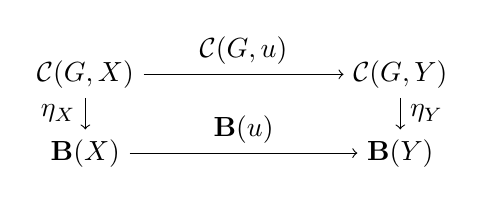
\begin{tikzpicture}[baseline=(current bounding box.center)]
\node (A) at (0,1) {$\mathcal C(G,X)$};
\node (B) at (4,1) {$\mathcal C(G,Y)$};
\node (C) at (0,0) {$\mathbf B(X)$};
\node (D) at (4,0) {$\mathbf B(Y)$};
\draw[->] (A) -- node[above] {$\mathcal C(G,u)$} (B);
\draw[->] (C) -- node[above] {$\mathbf B(u)$} (D);
\draw[->] (A) -- node[left] {$\eta_X$} (C);
\draw[->] (B) -- node[right] {$\eta_Y$} (D);
\end{tikzpicture}
\]
to commute. With \(\eta=\eta^a\) this is tautological: \(\mathbf B(u)\big(\mathbf B(f)(a)\big)=\mathbf B(u\!\circ\! f)(a)\). Naturality is thus a \emph{law-of-variation} principle: attribute-values at \(Y\) are not ad hoc stipulations but the transported values of attribute-data at \(X\) along \(u\). In particular, the value of \(\eta\) on a composite \(u\circ f\) is forced by its value on \(f\).

Read philosophically, naturality prevents “gerrymandered” positive predication. If an attribute is genuinely about \(G\)’s manifestation in the whole of \(\mathcal C\), then its predications must be \emph{compatible} with how objects and arrows hang together. The categorical setting elevates this compatibility from rhetoric to a precise coherence condition.

\subsection{The canonical element and anchoring at \texorpdfstring{$G$}{G}}
Every attribute \(\eta\) is anchored at \(G\) by the distinguished element \(a_\eta:=\eta_G(1_G)\in\mathbf B(G)\). Conversely, \(a\in\mathbf B(G)\) generates the entire attribute \(\eta^a\). This \emph{basepoint} perspective is not merely a convenience: it exhibits the sense in which cataphatic content about \(G\) is globally controlled by a single seed in \(\mathbf B(G)\).

We avoid over-interpretation. The canonical element does not, by itself, carry theological weight; it tracks how the naturality constraints condense a global family of assertions to one internal datum. The interpretation remains strictly \emph{in-model}: the identity \(1_G\) is the unique “probe of \(G\) by \(G\),” and its image through \(\eta\) fixes the whole attribute.

\subsection{Algebra on attributes and actions by endomorphisms}
When \(\mathbf B\) carries pointwise algebraic structure (e.g.\ each \(\mathbf B(X)\) is a commutative monoid and \(\mathbf B(u)\) is a homomorphism), the set of attributes \(\mathrm{Nat}(\mathcal C(G,-),\mathbf B)\cong\mathbf B(G)\) inherits the same algebra. Thus one can add, scale, or combine attributes whenever \(\mathbf B\) allows—useful for modeling \emph{aggregated} positive predications.

Moreover, \(\mathrm{End}(G)\) acts on attributes by precomposition on \(\mathcal C(G,-)\): given \(\alpha\in\mathrm{End}(G)\), define \((\eta\cdot\alpha)_X:=\eta_X\circ(-\circ\alpha)\). Under Yoneda, this corresponds to the action \(a\mapsto \mathbf B(\alpha)(a)\) on \(\mathbf B(G)\). This action anticipates the immanent-apophatic layer: endomorphisms modulate every manifestation of an attribute without themselves being new outward arrows \(G\to X\).

\subsection{Internalization: attributes as internal elements/predicates}
If \(\mathbf B\) lands in a topos \(\mathcal E\), then an attribute is literally an \emph{internal element} \(a:\mathbf 1\to \mathbf B(G)\) of \(\mathcal E\), with components \(\eta^a_X(f)=\mathbf B(f)\circ a\). In particular, when \(\mathbf B\) factors through the subobject fibration (so \(\mathbf B(X)\) are “predicates on \(X\)”), attributes become internally expressible predicates that vary naturally with \(X\).

This internal viewpoint clarifies the logical status of cataphatic predication: attributes live where the internal logic lives. It also sets up later limitations: once one counts attributes as internal predicates, undefinability results \citep{Tarski1956} constrain which global classifiers of “true attributes” can exist inside the same logic.

\subsection{Observational reading: attributes as probe responses}
There is a useful epistemic rephrasing. Think of each arrow \(f:G\to X\) as a \emph{probe} of \(X\) by \(G\). An attribute determined by \(a\in\mathbf B(G)\) assigns to every probe \(f\) the “response” \(\mathbf B(f)(a)\in\mathbf B(X)\). The naturality law says these responses compose: probing \(Y\) via \(u\circ f\) yields the transported response of probing \(X\) via \(f\).

In this sense, cataphatic data are \emph{response profiles} of all possible probes by \(G\). The profile is complete (in the functorial sense) once the anchor \(a\) is fixed. This reading stays within the structural stance: attributes record how \(G\) behaves as a universal tester across \(\mathcal C\).

\subsection{Examples and non-examples (sanity checks)}
In a thin category (preorder) the Hom-sets are singletons or empty. Then \(\mathcal C(G,-)\) is a principal upset, and attributes amount to specifying one element of \(\mathbf B(G)\), with little room for nontrivial variation: a reminder that interesting cataphatic structure requires non-thin morphism sets.

At the other extreme, in a presheaf-like setting where \(\mathbf B\) is already known to be representable (e.g.\ \(\mathbf B\cong \mathcal C(G,-)\) by construction), attributes coincide with endomorphisms of \(\mathcal C(G,-)\), hence with \(\mathbf B(G)\) as above. Between these poles lie the cases of interest: \(\mathbf B\) continuous but not obviously representable, where the existence step of \S\ref{sec:being} yields \(G\) and the cataphatic layer becomes substantive.

\subsection{Caveats: expressivity and definability}
Two caveats temper the cataphatic picture. First, the identification \(\mathrm{Nat}(\mathcal C(G,-),\mathbf B)\!\cong\!\mathbf B(G)\) captures only \emph{functorially coherent} predications; ad hoc or context-breaking assertions are excluded by design. Second, even within the coherent class, not every \emph{true} attribute may be internally \emph{definable} in a given logic; this is where incompleteness and undefinability (developed in \S\ref{sec:incompl}) become relevant.

These caveats are features, not bugs: they keep the cataphatic layer honest. The first ensures positivity respects the structure of \(\mathcal C\); the second flags principled limits on what any internal language can capture about \(G\), paving the way to the apophatic boundary. \citep{PseudoDionysius1987}

\section{Immanent-Apophatic Layer: Ineffable Core via Endomorphisms}\label{sec:apophatic}

\subsection{Endomorphisms and internal hom as the reflexive layer}
Fix a representing object \(G\) for \(\mathbf B\). The endomorphism monoid
\[
\mathrm{End}(G)\ :=\ \mathcal C(G,G)
\]
acts on each hom-set \(\mathcal C(G,X)\) by right composition:
\[
\mathcal C(G,X)\times \mathrm{End}(G)\ \longrightarrow\ \mathcal C(G,X),\qquad (f,\alpha)\ \mapsto\ f\circ \alpha.
\]
This action is compatible with composition in \(\mathcal C\): for \(u:X\to Y\) we have \((u\circ f)\circ \alpha = u\circ (f\circ \alpha)\). Thus the entire Hom–functor \(\mathcal C(G,-)\) is a \(\mathrm{End}(G)\)-module object in \([\mathcal C,\mathbf{Set}]\). Intuitively, \(\mathrm{End}(G)\) is the algebra of \emph{self-relations} of \(G\) that modulate every outward manifestation \(G\to X\) without producing new codomains.

If \(\mathcal C\) is enriched over a closed monoidal base \(\mathcal V\), this self-structure packages as an \emph{internal hom} object \([G,G]\in \mathcal V\). Then each enriched hom \(\mathcal C(G,X)\) carries a right \([G,G]\)-module structure by composition. This internalization will matter later: immanent-apophatic content becomes a \(\mathcal V\)-object acting on all cataphatic data but not itself an additional natural transformation \(\mathcal C(G,-)\Rightarrow \mathbf B\).

\subsection{Attributes are equivariant data; the self-action is not itself an attribute}
Recall that attributes are \(\eta:\mathcal C(G,-)\Rightarrow \mathbf B\), hence elements \(a\in \mathbf B(G)\). The \(\mathrm{End}(G)\)-action transports attributes via
\[
(\eta\cdot \alpha)_X\ :=\ \eta_X\circ(\,\_\,\circ\alpha)\qquad\text{corresponding to}\qquad a\ \mapsto\ \mathbf B(\alpha)(a).
\]
Thus attributes form a right \(\mathrm{End}(G)\)-set \(\mathbf B(G)\), and an attribute is \emph{equivariant} precisely when \(a\) is fixed by the action of a chosen submonoid of \(\mathrm{End}(G)\).

By contrast, the \emph{entire} self-action of \(\mathrm{End}(G)\) on \(\mathcal C(G,-)\) is not itself a single attribute. Any attribute must land in \(\mathbf B(-)\), while the self-action lands back in \(\mathcal C(G,-)\). One could try to \emph{encode} the action into \(\mathbf B\) by enlarging \(\mathbf B\), but doing so merely relocates the reflexive layer; it does not identify a natural transformation that \emph{is} the self-action. This mismatch—action on the Hom–profile versus a map into \(\mathbf B\)—is the first formal trace of ineffability.

\subsection{Opacity claim: no totalizer of the self-action}
Suppose for contradiction there were a single attribute \(\tau:\mathcal C(G,-)\Rightarrow \mathbf B\) that \emph{classifies} the full \(\mathrm{End}(G)\)-action in the sense that, for every \(X\), the family \(\big(\tau_X(f\circ \alpha)\big)_{\alpha\in\mathrm{End}(G)}\) internally recovers the map \(\mathrm{End}(G)\to \mathcal C(G,X)\), \(\alpha\mapsto f\circ \alpha\), up to isomorphism in \(\mathbf B(X)\). In expressive settings this would give, by parametrization in \(f\) and naturality in \(X\), a single internal predicate that \emph{tracks all self-modulations of all manifestations at once}. In \S\ref{sec:incompl} we explain why fixed-point/undefinability templates obstruct such totalizers: a uniform internal truth about “all modulations of all manifestations” is prohibited by the very mechanisms that produce self-reference.

The moral here is modest: it is not that no information about the self-action can be cataphatically expressed; rather, there is no \emph{single} coherent attribute that swallows the entire reflexive algebra without collapse. The immanent-apophatic core is the residual that eludes such collectivization.

\subsection{Orbits and invariants: what the self-action hides and reveals}
The \(\mathrm{End}(G)\)-action on \(\mathbf B(G)\) organizes attributes into \emph{orbits} and \emph{invariants}. An orbit collects attributes that differ only by precomposition on their anchor: \(a\sim a'\) if \(a'=\mathbf B(\alpha)(a)\). The fixed-point set
\[
\mathbf B(G)^{\mathrm{End}(G)}\ :=\ \{\,a\in\mathbf B(G)\mid \mathbf B(\alpha)(a)=a\ \ \forall\,\alpha\in\mathrm{End}(G)\,\}
\]
records attributes insensitive to any self-modulation of \(G\). These are the \emph{maximally stable} cataphatic claims; everything else varies along hidden degrees of freedom governed by \(\mathrm{End}(G)\).

This suggests a methodology: positive talk about \(G\) that aspires to universality should, at minimum, be invariant under \(\mathrm{End}(G)\). The immanent-apophatic layer then appears as the quotienting process “attribute modulo self-action.” The larger the action (e.g.\ if \(\mathrm{End}(G)\) is rich), the thinner the invariant core—mirroring the intuition that the more intrinsic self-relation a source has, the less can be stably said about it outwardly.

\subsection{Automorphisms vs.\ general endomorphisms}
The subgroup \(\mathrm{Aut}(G)\subseteq\mathrm{End}(G)\) acts by reparameterizations that are invertible. Invariants under \(\mathrm{Aut}(G)\) capture statements insensitive to mere \emph{renaming} of how \(G\) maps to itself. Non-invertible endomorphisms, however, encode genuine \emph{foldings} or \emph{quotients} of the self-relation; their presence typically enlarges orbits beyond mere symmetries and thus deepens opacity.

In many examples, \(\mathrm{Aut}(G)\) already acts transitively on a large portion of \(\mathbf B(G)\), so only coarse features survive. When non-invertible endomorphisms abound (e.g.\ idempotents, nilpotents), the stratification of attributes by orbits becomes even coarser, further curtailing what can be positively stabilized.

\subsection{Enriched picture: the internal hom \texorpdfstring{$[G,G]$}{[G,G]} as apophatic object}
In a closed \(\mathcal V\)-enriched setting, each component \(\mathcal C(G,X)\) is a right \([G,G]\)-module. Attributes correspond to \(\mathcal V\)-natural transformations \(\mathcal C(G,-)\Rightarrow \mathbf B\), hence to \(\mathcal V\)-elements of \(\mathbf B(G)\). The \([G,G]\)-action transfers along \(\mathbf B\) via \(\mathbf B(\_):[G,G]\to [\mathbf B(G),\mathbf B(G)]\).

This allows a sharper statement: the immanent-apophatic core is now literally the \(\mathcal V\)-object \([G,G]\) whose module action on \(\mathcal C(G,-)\) is ubiquitous yet whose full structure is not itself a \(\mathcal V\)-natural map into \(\mathbf B\). One can study centers, idempotents, and spectra of \([G,G]\) to measure degrees of intrinsic self-structure; each such invariant controls how much of \(\mathbf B(G)\) can be stabilized.

\subsection{Reader/Exponent monad viewpoint (when cartesian closed)}

If \(\mathcal C\) is cartesian closed, the assignment $T(X):=X^{G}$ forms a (Reader) monad with unit $\eta_X:x\mapsto (\lambda g.\,x)$ and multiplication 
$\mu_X:(X^{G})^{G}\cong X^{G\times G}\xrightarrow{(-)\circ \Delta}X^{G}$ given by precomposition with the diagonal $\Delta:G\to G\times G$.

Seen this way, cataphatic data are \emph{readers} of \(G\)-state, whereas the apophatic layer is the algebra of \emph{reindexings} of that state by self-maps of \(G\). Attempting to collapse all reindexings to a single attribute amounts to seeking a global evaluator for all contexts, which runs afoul of the fixed-point/undefinability boundaries discussed later.

\subsection{Local--global tensions (sheaf settings) and gluing failures}
In a sheaf topos, apophaticity can manifest as a failure of global sections for certain internal objects. One may have abundant \emph{local} attributes (sections of \(\mathbf B(G)\) over a cover) that cannot be glued to a \emph{global} attribute invariant under \(\mathrm{End}(G)\). The internal hom \([G,G]\) may be locally trivial yet globally nontrivial, obstructing any uniform naturalization of the reflexive layer.

This sheaf-theoretic perspective aligns well with negative theology: what can be said \emph{here and now} (locally) may not globalize across the entire site without contradiction or loss. The obstruction lives not in a missing definition but in the geometry of the index category and the nontriviality of the internal automorphism sheaf of \(G\).

\subsection{A schematic ``no-collapse'' template}
We record a general template (details deferred to \S\ref{sec:incompl}): suppose the internal logic interprets enough arithmetic and that \(\mathbf B\) is rich enough to encode truth-like predicates about attributes. Any attempt to define a single internal predicate \(\mathsf{AllAttr}\) that, for every \(X\) and \(f:G\to X\), uniformly decides the orbit of \(\eta_X(f)\) under all \(\alpha\in\mathrm{End}(G)\) leads to a Lawvere-style diagonal fixed point. This yields either inconsistency or incompleteness, showing that such a totalizer cannot exist internally.

The upshot is precise: \emph{some} aspects of the self-action can be encoded cataphatically (e.g.\ invariants, orbits relative to a submonoid), but there is no internal master-attribute that \emph{completely} captures the reflexive layer without stepping outside the system.

\subsection{Energeia vs.\ ousia}
Without committing to doctrinal theses, one may use a familiar vocabulary to summarize: the cataphatic layer (naturals) corresponds to \emph{energeiai}—modes in which \(G\) is manifest in and through other objects. The immanent-apophatic layer corresponds to an \emph{ousia}-like self-relatedness formalized by \(\mathrm{End}(G)\) or \([G,G]\), present in every manifestation by action, yet not itself reducible to a manifestation.

We keep this at the level of disciplined analogy. The mathematics supplies a clean distinction—external natural transformations versus internal self-action—and the analogy merely labels the sides. The subsequent incompleteness layer explains why the boundary resists systematic elimination.

\subsection{What the immanent-apophatic layer \emph{does} for the program}
Formally, the immanent-apophatic layer functions as a \emph{control knob} on positive predication: it tells us which attributes are stable (invariants), which are context-sensitive (orbits), and why certain hoped-for uniformities (totalizers) provably fail. Conceptually, it prevents overreach: even with a representing object in hand, the system itself contains a reflexive algebra that cannot be “said” in one natural breath. Together with Löb's constraint on internal provability \citep{Loeb1955}, these ceilings ensure that necessity in our register remains a disciplined, non-trivial modality rather than a surrogate for omniscient truth.

This is the sense in which ineffability is not a romantic flourish but a structural fact: the reflexive content of the source object is \emph{constitutively} different in type from its outward manifestations. The next section shows that self-reference and undefinability make this difference sticky even in very expressive internal logics.

\section{Incompleteness and Undefinability Boundaries}\label{sec:incompl}

\subsection{Lawvere-style fixed points and diagonal schemas for attributes}
We now make precise the self-reference pressure already implicit in the immanent-apophatic layer. Work in a cartesian closed ambient (e.g.\ a CCC or an elementary topos), and assume the internal logic is expressive enough to talk about predicates on attributes. Lawvere’s fixed-point template says: given a weak point-surjection \(e:A\to \Omega^{A}\) and any endomap \(t:\Omega\to\Omega\), there exists \(p\in\Omega\) with \(p \leftrightarrow t(p)\). Intuitively, once your universe can encode “properties of properties” with sufficient evaluation structure, diagonal sentences appear by force.

To apply this schematically to attributes, take \(A\) to be a type that \emph{codes} (suitably) the class \(\mathbf B(G)\) of cataphatic anchors (recall \(\mathrm{Nat}(\mathcal C(G,-),\mathbf B)\cong \mathbf B(G)\)). An internal “truth test” for attributes is an arrow \(\mathsf{P}:\mathbf B(G)\to\Omega\) and, by currying, compositional gadgets that combine \(\mathsf{P}\) with reindexings induced by endomorphisms of \(G\) (\S\ref{sec:apophatic}). Under mild surjectivity/exponentiability hypotheses, Lawvere’s template yields a diagonal \(d\) with \(d \leftrightarrow t(d)\) for a choice of \(t\) derived from \(\mathsf{P}\). Choosing \(t\) to negate, or otherwise oppose, what \(\mathsf{P}\) asserts about diagonals produces liar-/Curry-like pathologies unless \(\mathsf{P}\) is restricted. Thus any attempt to install a \emph{total} internal classifier for attribute-truth invites fixed points that either force incompleteness (withheld verdicts) or inconsistency (collapse).

The moral is modest but sharp: even before invoking arithmetic encodings, the mere presence of exponentials and evaluation already bounds what a single internal “truth-of-attributes” device can do. In effect, the diagonal mechanism guarantees a residue of cataphatic content that cannot be globally regimented. This residue is where the immanent-apophatic layer of \S\ref{sec:apophatic} lives: not because we refuse to speak, but because the structure itself prevents a total story.

\subsection{Tarskian undefinability for internal attribute truth}
When the internal logic interprets enough arithmetic (e.g.\ there is an NNO and induction up to a certain strength), Tarski-style theorems \citep{Tarski1956} rule out a truth predicate definable \emph{in the same language} that correctly classifies all internal sentences of that language. Translating the pattern to our setting: fix a formal language sufficient to express statements about \(\mathbf B(G)\), about the naturality constraints that extend anchors to attributes, and about their transport along morphisms. If we could define within that language a predicate \(\mathsf{TrueAttr}(a)\) that holds exactly of anchors \(a\in\mathbf B(G)\) whose induced natural transformations state true cataphatic claims, we could carry out a Gödel–Tarski diagonal to contradict \(\mathsf{TrueAttr}\)’s adequacy. 

Concretely, the undefinability barrier says that \emph{no} single internal subobject of \(\mathbf B(G)\) decidably carves out the “true” anchors for all attribute-statements expressible in the same system. Any workable device must either be \emph{partial} (fail to classify some cases), \emph{hierarchical} (live in a stronger metalanguage), or \emph{modal} (shift from truth to provability). This dovetails with the Lawvere template: diagonal self-application is the engine; Tarski’s theorem names the boundary.

Hence, the thought experiment cannot end with “select the true attributes and be done.” The best one can do \emph{internally} is to accept stratified, partial, or modal surrogates. The immanent-apophatic reading then receives a theorem-backed gloss: ineffability is the ineliminable gap between what the internal language can certify and the global coherence the structure hints at.

\subsection{Provability as a disciplined necessity: Löb-style constraints}
A standard way to \emph{work around} undefinability is to replace truth by a \emph{provability} (or necessity) operator \(\Box\) satisfying Hilbert–Bernays/Löb derivability conditions. Internally, treat \(\Box \varphi\) as “\(\varphi\) is derivable in a sound but incomplete theory of the internal logic.” Then Löb’s principle \citep{Loeb1955}
\[
\Box(\Box \varphi \rightarrow \varphi) \ \rightarrow\ \Box \varphi
\]
becomes available and yields a controlled route to “necessary” cataphatic claims: whenever an attribute \(\eta\) can \emph{self-endorse} its admissibility in the required way, \(\Box \text{Attr}(\eta)\) follows.

Two caveats enforce discipline. First, \(\Box\) does not collapse to truth (by design), so “necessary” here is internal-provability, not metaphysical necessity. Second, Curry-like pathologies are avoided precisely by staying within a provability regime that blocks \(\varphi \Rightarrow \Box\varphi\) in general. The gain is a usable dial: one can mark a stable core of \(\Box\)-attributes without claiming a total truth predicate, harmonizing the cataphatic layer with the incompleteness ceiling.

\subsection{Partial truth and reflection: safe, non-totalizing expansions}
Between naked truth and modal provability lie \emph{partial} and \emph{reflective} strategies. Kripke-style fixed points for partial truth (e.g.\ Strong Kleene valuations) allow an internally defined predicate \(\mathsf{T}\) that correctly classifies many attribute-statements while leaving some \emph{undefined}. In our context, \(\mathsf{T}\) can cover a robust fragment of cataphatic discourse and politely abstain at diagonal pinch-points, preserving consistency.

Reflection schemata \citep{Feferman1960} offer a complementary, \emph{ascending} method: from a base theory \(T\), add uniform reflection principles (“if \(T\) proves \(\varphi\), then \(\varphi\)”) for a calibrated class of formulas (e.g.\ \(\Sigma_n\)). Iterating reflection expands the certifiable cataphatic horizon without ever producing a single omniscient classifier. Both techniques respect the immanent-apophatic boundary: the horizon recedes as you advance, not because of poverty of language, but because of principled non-totalizability.

\subsection{A no-totalizer template for the self-action}\label{subsec:nototal}
We now formulate a schematic “no-totalizer” claim that ties together \S\ref{sec:apophatic} and the present section. Suppose the internal logic can encode:
\begin{enumerate}[leftmargin=2em,label=(\roman*)]
  \item an evaluation of anchors along arrows, \( \operatorname{ev}_X:\mathbf B(G)\times \mathcal C(G,X) \to \mathbf B(X)\) (the Yoneda transport),
  \item the \(\mathrm{End}(G)\)-action on anchors, \( \rho:\mathrm{End}(G)\times \mathbf B(G)\to \mathbf B(G)\), and
  \item a truth-like predicate \(\mathsf{Good}_X\) that attempts to judge, uniformly in \(X\), the orbit-behavior of \(\operatorname{ev}_X\big(\rho(-,a),f\big)\) under all \(\alpha\in\mathrm{End}(G)\).
\end{enumerate}
If there existed a \emph{single} internal device \(\mathsf{AllAttr}\) that, for all \(X\) and \(f:G\to X\), determined the orbit-equivalence class (or even a canonical representative) of the family \(\{\operatorname{ev}_X(\rho(\alpha,a),f)\}_{\alpha}\) in a way natural in \(X\), then—under mild surjectivity/expressivity hypotheses—the Lawvere diagonal applied to \(\mathsf{AllAttr}\) yields a fixed-point obstruction. One concludes that no such uniform, natural totalizer exists \emph{internally}; at best, one has partial/cased-based classifiers or external (meta-level) selections.

This template should be read as a programmatic constraint rather than a finished theorem (details depend on the precise internal codings). Its significance is conceptual: the self-action’s full algebra cannot be reified as a single cataphatic attribute without violating the fixed-point/undefinability boundaries. That is exactly the sense in which an “ineffable core” \emph{remains} after representability.

\subsection{Local--global obstructions in sheaf/stack settings}
In sheaf-theoretic environments, a second family of boundaries arises from geometry rather than diagonalization. Let \(\mathcal E=\mathbf{Sh}(\mathcal S)\) be a sheaf topos on a site \(\mathcal S\), and consider the internal automorphism object \(\underline{\mathrm{Aut}}(G)\) and its action on \(\mathbf B(G)\). Even when attributes cover locally (every point of \(\mathcal S\) admits rich cataphatic data), global invariants may \emph{fail to glue} if the associated \(\underline{\mathrm{Aut}}(G)\)-torsor is nontrivial. The obstruction is measured by a cohomology class; selecting a global invariant attribute amounts to choosing a global section of a twisted object, which may not exist.

This shows that immanent-apophatic residue can be \emph{geometric}: not every locally coherent positive predication globalizes. The sheaf picture thus complements the logical ceilings: one blocks totalization by cohomological torsion, the other by diagonal/undefinability. \citep{Giraud1971, Goedel1931} Both converge on the same moral—no single, internally available “view from nowhere” collects all manifestations.

\subsection{Meta/object-level hygiene and scope of the boundary claims}
A recurring danger is to confuse \emph{meta}-level arguments (about the model) with \emph{object}-level claims (in the model). Our use of Lawvere/Tarski is internal where possible but inevitably appeals to meta-reasoning to set up codings and adequacy. The safe summary is: within any sufficiently expressive categorical environment, either (i) global attribute-truth is \emph{not} definable internally, or (ii) internal truth devices are partial/modal/stratified and cannot be tightened to totality without loss.

Accordingly, our boundary claims are \emph{negative existentials} about internal classifiers, not declarations about what is ultimately real. They tell you which proof shapes cannot exist given your structure, and thereby justify the apophatic layer as a structural feature of the model. In keeping with our critical register, the point is to chart where formal methods \emph{must} hand back to philosophical discretion and background metaphysics.

\subsection{Takeaway for the overall narrative}
The existence step (\S\ref{sec:being}) gives a representing object \(G\). The cataphatic layer (\S\ref{sec:cataphatic}) organizes positive predication as naturals out of \(\mathcal C(G,-)\). The immanent-apophatic layer (\S\ref{sec:apophatic}) identifies the reflexive self-action that modulates every manifestation. The present section shows that \emph{even} in expressive logics there is no coherent way to compress all that positive data into a single, internally definable totality: diagonal and geometric obstructions ensure remainder.

Thus, the negative theology upgrade is not rhetorical flourish—it is the boundary drawn by fixed points, undefinability, and (in geometric settings) torsion of gluing. The philosophical upshot matches the formal one: what can be naturally said about \(G\) is rich but inherently non-exhaustive.

\subsection{Fibrational modality and Löb reflection on attributes}\label{subsec:fibrational-gl}
 
\paragraph{Motivation.}
Philosophically, a fibrational modality turns vague talk of “necessity’’ into a \emph{disciplined} operator on claims that are already natural across contexts. By lifting $\Box$ fiberwise to attributes, we separate (i) what is \emph{true} about a manifestation of $G$ from (ii) what is \emph{stably provable/robust} under reindexing, refinement, and pullback. Löb’s reflection at the attribute level then explains why some cataphatic claims form a \emph{stable core} (closed under proof and change of context) without inflating them into metaphysical necessity: $\Box$ remains a structural/epistemic guardrail, not an oracle of truth. At the same time, compatibility with the self–action of $G$ shows that modal stability and immanent-apophatic modulation \emph{coexist}: we can mark what endures under proof while acknowledging the reflexive residue that no proof regimen captures. Practically, this blocks modal overreach (Curry–style collapses), clarifies which assertions survive passage between sites or slices, and yields a common yardstick for comparing “necessary’’ claims across different ambient logics. In short, the fibrational view upgrades “laws of discourse’’ from rhetoric to structure: it makes precise why some predicates deserve the honorific “necessary’’ in our register, and why even then the ceilings (Lawvere/Tarski) keep necessity from masquerading as omniscient truth.

\paragraph{Setting.}
Let $p:\mathcal P\!\to\!\mathcal C$ be a (first–order) hyperdoctrine: for each $X\in\mathcal C$ a Heyting algebra $\mathcal P(X)$ of predicates on $X$, with reindexing $u^\ast:\mathcal P(Y)\!\to\!\mathcal P(X)$ for $u:X\!\to\!Y$ (and the usual adjoints where available). Assume a \emph{fibred comonad} $\Box$ on $p$:
\[
\epsilon:\Box\Rightarrow \mathrm{Id},\quad \delta:\Box\Rightarrow \Box\Box,\qquad
\text{cartesian over }\mathcal C,\ \text{so }u^\ast\circ \Box_Y\cong \Box_X\circ u^\ast.
\]
Intuitively, $\Box$ is a necessity/derivability operator (e.g.\ from a Lawvere–Tierney topology \citep{Lawvere1971Quantifiers} or a modal hyperdoctrine \citep{Jacobs1999, Johnstone2002Elephant}).

\paragraph{Attributes with predicates.}
Let $\mathsf H_G:=\mathcal C(G,-)$ be the covariant Hom–functor. An \emph{attribute} with values in the doctrine is a natural transformation
\[
\eta:\ \mathsf H_G\Longrightarrow \mathcal P\,,
\qquad\text{i.e.}\quad
\eta_X:\ \mathcal C(G,X)\longrightarrow \mathcal P(X),
\]
natural in $X$ (so $\eta_Y(u\circ f)=u^\ast(\eta_X(f))$). Write $\mathrm{Attr}_\mathcal P(G):=\mathrm{Nat}(\mathsf H_G,\mathcal P)$ for the set (or poset) of such attributes.

\paragraph{Lift of the modality.}
Define $\Box_{\!\mathrm{Attr}}:\mathrm{Attr}_\mathcal P(G)\!\to\!\mathrm{Attr}_\mathcal P(G)$ by
\[
\big(\Box_{\!\mathrm{Attr}}\eta\big)_X\ :=\ \Box_X\!\big(\eta_X\big)\,.
\]
Because $\Box$ is fibred (commutes with reindexing up to coherent iso), $\Box_{\!\mathrm{Attr}}\eta$ is again natural in $X$. The comonad laws of $\Box$ lift pointwise, so $\Box_{\!\mathrm{Attr}}$ is a comonad on attributes.

\paragraph{Löb reflection at attribute level.}
Assume the doctrine validates GL fibrewise:
\[
\forall X\ \forall P\in\mathcal P(X):\quad \Box_X\!\big(\Box_X P \Rightarrow P\big)\ \Rightarrow\ \Box_X P\,.
\]
Then the same reflection holds for attributes:
\[
\Box_{\!\mathrm{Attr}}\!\Big(\,\Box_{\!\mathrm{Attr}}\eta\ \Rightarrow\ \eta\,\Big)\ \Rightarrow\ \Box_{\!\mathrm{Attr}}\eta\,,
\qquad \eta\in \mathrm{Attr}_\mathcal P(G),
\]
where $\Rightarrow$ is computed pointwise in the Heyting fibres $\mathcal P(X)$. In particular, the $\Box$–coalgebras inside $\mathrm{Attr}_\mathcal P(G)$ form a \emph{provability–stable} core of cataphatic claims, without collapsing necessity to truth.

\paragraph{Compatibility with self–action.}
For $\alpha\in\mathrm{End}(G)$, define the right action $(\eta\cdot\alpha)_X:=\eta_X(\,{-}\circ \alpha)$. Since $\Box$ is fibred,
\[
\Box_{\!\mathrm{Attr}}(\eta\cdot\alpha)\ =\ \big(\Box_{\!\mathrm{Attr}}\eta\big)\cdot \alpha\,,
\]
so the immanent-apophatic self–modulation (by $\mathrm{End}(G)$) and the modal reflection (by $\Box$) \emph{coexist} without interference.

\section{Weakened Universality: Where the Action Is}\label{sec:intermediate}
\noindent
The strict case $\mathbf B\cong \mathcal C(G,-)$ is mathematically clean but, we suggest, \emph{not} where the most interesting philosophy lives. The richest structure (and the most revealing limits) arises in the \emph{intermediate regimes}---where full representability fails but universality persists in weakened or stratified forms. Universality persists in a weakened form whenever finite coherence holds; it fails only when even finite compatibility breaks. This section systematizes those regimes, pairs each with an ontological/theological gloss, and argues that they are not consolation prizes but the core phenomenology of ``being as structure.'' 

\subsection{Pro-/Ind-representability: the Transcendent-Apophatic Middle}\label{subsec:proind}
\paragraph{Form.}
A functor $F:\mathcal C\to\mathbf{Set}$ is \emph{pro-representable} when
\[
F \ \simeq\ \varinjlim_{i}\, \mathcal C(G_i,-),
\]
for a cofiltered system $(G_i)_{i}$ in $\mathcal C$ (so a filtered colimit of representables). 
Dually, it is \emph{Ind-representable} when
\[
F \ \simeq\ \varprojlim_{j}\, \mathcal C(H_j,-).
\]
(Here $\mathrm{Ind}(\mathcal C)$ supplies formal filtered colimits; maps out of such colimits induce limits of representables.) \citep{ArtinMazur1969}

\paragraph{Ontological gloss.}
Pro-representability formalizes a \emph{transcendent-apophatic limit}: the universal source is approached by a \emph{via negativa} of coherent refinements (ever more discriminating finite ``names'') yet never collapses to a single object. Ind-representability reads cataphatically as \emph{emanation/unfolding}: a plenitude expressed by a filtered colimit of manifestations. The pair captures a principled dialectic: contraction toward ineffability vs.\ expansion into expression.

\paragraph{Immanent-apophatic layer.}
For $P=(G_i)\in \mathrm{Pro}(\mathcal C)$ the reflexive algebra becomes a pro-monoid
\[
\mathrm{End}_{\mathrm{Pro}(\mathcal C)}(P)
=\varprojlim_{j}\,\varinjlim_{i}\,\mathcal C(G_i,G_j).
\]
a tower of coherent self-relations visible at every finite stage yet never realized at once---an exact structural surrogate for ``ineffable selfhood.'' 

\subsection{Local Representability and Gluing: Sheaf/Stack Regimes}\label{subsec:local}
\paragraph{Form.}
$\mathbf B$ is representable on a cover but not globally; after sheafification/stackification one recovers representability by a (higher) object. Local charts $U_i$ carry representers $G_i$ with descent data on overlaps, but the global obstruction (cocycle) prevents a single $G$.

\paragraph{Ontological gloss.}
This is a \emph{dependence realism}: intelligibility is local and relational, while any attempt to crystallize a global essence fails. It resonates with a skeptical (non-nihilist) Middle Way: there is order in the overlaps (transition isomorphisms), not a single self-subsistent core.

\paragraph{Immanent-apophatic layer.}
The ``ineffable'' appears as a \emph{failure to glue}: torsors and cohomology classes measure precisely why no global attribute/representer exists despite flawless local coherence.

\subsection{Higher/Stacky Representability: Universality up to Equivalence}\label{subsec:stacky}
\paragraph{Form.}
When $\mathbf B$ is groupoid- or $\infty$-groupoid-valued (symmetries/gauge), representability holds as a \emph{stack}: $\mathbf B\simeq \mathrm{Map}(\mathcal G,-)$ in a suitable $(\infty,1)$-topos. Universality is preserved but \emph{only up to equivalence}. \citep{Lurie2009HTT}

\paragraph{Ontological gloss.}
Being is \emph{essentially relational}: identity is determined modulo symmetry. The ``one'' is not a rigid object but a classifying stack whose automorphism $\infty$-group \emph{is} part of what is universal.

\paragraph{Immanent-apophatic layer.}
$\mathrm{Aut}(\mathcal G)$ becomes the reflexive core; the larger the symmetry, the thinner the invariant cataphatic content---a quantifiable apophasis.

\subsection{Ind–Pro (Tate) Stacky Representability: Hybrid Universality}\label{subsec:indpro-stacky}
\paragraph{Form.}
In many stacky settings the most faithful “representer’’ is neither a single stack nor a pure pro– or Ind–object, but an \emph{Ind–Pro (Tate) moduli object}. Concretely, in a suitable $(\infty,1)$\nobreakdash-topos one often has a presentation
\[
\mathbf B \;\simeq\; \operatorname*{colim}_{i\in I}\ \operatorname*{lim}_{j\in J_i}\ \mathrm{Map}(-,\mathcal G_{i,j}),
\]
with $I$ filtered (Ind–direction), each $J_i$ cofiltered (pro–direction), and each stage $\mathcal G_{i,j}$ a geometric (possibly derived) stack. Intuitively: \emph{formal/refinement} data accumulate along the pro–tower, while \emph{large/exhaustion} data assemble along the Ind–colimit.

\paragraph{When and why.}
This hybrid appears when $\mathbf B$ satisfies descent (stackiness) and finite–limit coherence (pro side), while also commuting suitably with filtered colimits or Noetherian approximation (Ind side). \citep{Rydh2015Noetherian} Typical sources: field theories with both formal boundary/jet towers and increasing domain/exhaustion; derived moduli combining deformation thickenings and unions of strata; infinite–dimensional symmetry (loop/jet/Tate phenomena).

\paragraph{Collapses (if available).}
Under additional compactness/smallness or geometricity hypotheses, the Ind–Pro representer may \emph{descend} to a pure pro–stack, a pure Ind–stack, or even a single stack $\mathcal G$:
\[
\mathbf B \simeq \mathrm{Map}(-,\mathcal G)\,.
\]
Absent such hypotheses, the Ind–Pro shape is canonical and retains explanatory contrast: refined stages and large assemblies are tracked separately.

\paragraph{Ontological gloss.}
Being discloses itself along \emph{two asymptotic axes}. The pro–direction encodes \emph{refinement to interiority} (ever finer, formally thickened manifestations); the Ind–direction encodes \emph{expansion to plenitude} (ever larger, exhaustively assembled contexts). The universal source is thus not a rigid \emph{one} but a \emph{Tate–classifying horizon}: an asymptotic generator whose modes are given by compatible families across refinement and expansion. To “participate in being’’ is to stabilize under both movements—what is sayable appears at finite stages; what remains unsayable is the limit–only self–relation that guides them. In this sense, weakened universality is not dilution but a \emph{layered} ontology: interior depth (pro) and outward plenitude (Ind) held together by a single, stacky universal role.

\paragraph{Immanent-apophatic layer.}
The reflexive core becomes a Tate–like automorphism group
\[
\mathrm{Aut}\!\left(\operatorname*{colim}_i\operatorname*{lim}_j \mathcal G_{i,j}\right)
\;\simeq\;
\operatorname*{lim}_{j}\ \operatorname*{colim}_{i}\ \mathrm{Aut}(\mathcal G_{i,j}),
\]
an inverse–limit/filtered–colimit symmetry realized at no finite stage. It modulates every staged attribute while remaining “only at the limit’’—a deepened quantifiable apophasis.

\subsection{Derived/Geometric Representability: Universality with Deformation}\label{subsec:derived}
\paragraph{Form.} 
Add derived structure (deformations, obstruction theory) to impose geometricity/descent; the solution functor becomes representable by a derived (higher) object. \citep{ToenVezzosiHAG}

\paragraph{Ontological gloss.}
Dependence includes \emph{counterfactual neighborhoods}: ``what-being-would-be-under-perturbation'' is part of being. Universality arises \emph{with} its tangent/obstruction data, not after stripping it away.

\paragraph{Immanent-apophatic layer.}
Hidden self-structure often externalizes as obstruction classes: the impossibility of flattening deformations is precisely where ineffability lives.

\subsection{Partial and Modal Truth: Provability Layers}\label{subsec:modal}
\paragraph{Form.}
Internal modalities (Lawvere--Tierney, hyperdoctrinal comonads) induce a comonad $\Box_{\mathrm{Attr}}$ on attributes; GL/Löb governs reflection. ``Necessary'' attributes are $\Box$-coalgebras; ``possible'' ones sit below. \citep{Lawvere1971Quantifiers}

\paragraph{Ontological gloss.}
This stratifies perfections by \emph{derivability}, not omniscient truth: necessity = provability in a disciplined internal theory. The apophatic ceiling (Tarski/Lawvere) remains intact; modality threads a safe middle path.

\paragraph{Immanent-apophatic layer.}
No total truth functor exists; necessity cannot collapse to truth. The gap is theorem-backed, not rhetorical.

\subsection{Undecidable representability and the pro–shadow}\label{subsec:undecidable}
\paragraph{Form.}
For left–exact $\,\mathbf B:\mathcal C\to\mathbf{Set}\,$ with $\mathcal C$ essentially small and finite–limit, there is a canonical \emph{pro–presentation}
\[
\mathbf B\ \simeq\ \varinjlim_{i}\ \mathcal C(G_i,-)\,,
\]
so universality exists at least \emph{asymptotically}. Whether this pro–object descends to a single representing object $G\in\mathcal C$ (strict representability) is, in general, not settled \emph{inside} the attribute register and may be hard in two distinct senses:
\begin{enumerate}[leftmargin=2em,label=(\alph*)]
\item \textbf{Algorithmic undecidability.} If the attribute data are infinite but effectively given (computable fibres and structure maps), there is \emph{no uniform algorithm} that decides from those data whether a single $G$ exists (Theorem~\ref{thm:alg-status}(b)); in the finite, extensional case it is decidable (Theorem~\ref{thm:alg-status}(a)).
\item \textbf{Set–theoretic independence.} In many natural ambient categories, strict representability (or its higher/stacky analogues) can depend on additional axioms (solution–set/choice, large–cardinal principles); thus its truth may be independent of a modest base theory.
\end{enumerate}
In either case, the \emph{canonical} object one can point to without extra assumptions is the \emph{pro–shadow} $P=\{G_i\}$.

\paragraph{Ontological gloss.}
This yields a \emph{transcendent-apophatic horizon}: the universal role is coherent and present as a limit of approximations, while its immanence as a single $G$ is not fixed by the internal data (and may be undecidable). The pro–shadow objectifies a \emph{regulative ideal}: it governs manifestations and comparisons, even where a single source is not obtainable.

\paragraph{Reflexive layer in the undecidable regime.}
Replace the endomorphism monoid $\mathrm{End}(G)$ by the \emph{pro–endomorphism} monoid
\[
\mathrm{End}(P)\ \cong\ \varprojlim_{j}\ \varinjlim_{i}\ \mathcal C(G_i,G_j)\,,
\]
the inverse–limit symmetry that modulates every staged manifestation. This is the natural “immanent–apophatic” core when only the pro–shadow is available.

\subsection{Where and why strict universality fails to present}\label{subsec:diagnostics}
\paragraph{Structural symptoms.}
\begin{itemize}[nosep,leftmargin=2em]
\item \emph{Size breaks.} $\int\!\mathbf B$ lacks a \emph{small} weakly initial family or cannot be promoted to an initial object $\Rightarrow$ universality is too large/indefinite at this level.
\item \emph{Continuity breaks.} $\mathbf B$ fails (finite) limits $\Rightarrow$ context–sensitivity/gluing failures; expect only local or staged universality.
\item \emph{Symmetry/quotient pressure.} Nontrivial identifications (gauge) push from sets to groupoids/stacks; representability migrates to a higher ambient.
\item \emph{Computational ceiling.} With effective infinitary data, even when (finite) coherence holds, strict representability is not uniformly decidable from attribute–level input (Theorem~\ref{thm:alg-status}(b)).
\end{itemize}

\paragraph{Routing.}
Each symptom points to a principled repair:
\begin{itemize}[leftmargin=2em]
\item \emph{Pro/Ind completion} for asymptotic universality (take the pro–shadow $P$ or its Ind dual).
\item \emph{Sheaf/stack upgrade} to restore gluing and quotient by symmetry (local $\to$ global up to equivalence).
\item \emph{Derived/geometric structure} to track deformation/obstruction when universality lives with tangent data.
\item \emph{Modal discipline} (\S\ref{subsec:fibrational-gl}) to mark a stable provability core when truth cannot be totalized.
\end{itemize}
The point is not to force a single $G$ at all costs, but to place universality where the structure earns it and to make explicit which extra assumptions move you across the decidability/definability boundary.

\subsection{Comparative Table: Regimes and Readings}\label{subsec:table}
\begin{center}\small
\begin{tabular}{p{3.1cm}p{4.2cm}p{4.2cm}p{4.2cm}}
\hline
\textbf{Regime} & \textbf{Categorical form} & \textbf{Cataphatic content} & \textbf{Apophatic content / gloss}\\
\hline
Strict representability & $\mathbf B\!\cong\!\mathcal C(G,-)$ & Naturals $\leftrightarrow \mathbf B(G)$ & $\mathrm{End}(G)$ as reflexive core; classical universality\\
Pro-/Ind- & $\varprojlim \mathcal C(G_i,-)$ / $\varinjlim \mathcal C(G_i,-)$ & Compatible staged attributes & Pro-end $\mathrm{End}(P)$; limit-ideal universality (via negativa)\\
Local/sheaf & Representable on cover; descent & Local attributes; torsors on overlaps & Gluing obstructions; dependence realism (no global essence)\\
Stacky/higher & $\mathbf B\simeq \mathrm{Map}(\mathcal G,-)$ & Invariants up to equivalence & Automorphism $\infty$-group; identity-as-symmetry\\
Derived/geometric & Geometric/derived stack & Attributes with deformation data & Obstruction classes as hidden self-structure\\
Modal/partial & $\Box_{\mathrm{Attr}}$ on naturals & $\Box$-stable (provable) perfections & No total truth; GL reflection as guardrail\\
\hline
\end{tabular}
\end{center}

\subsection{Case: Information Geometry in Miniature}\label{subsec:ig-mini}
\paragraph{Motivation.}
Information geometry provides an ideal ``sanity check” for the framework: it is neither theological nor trivial. Its core results—representability of the pair-functor by the binary simplex, the recovery of 
\(f\)-divergences as natural attributes, the Fisher–Rao metric as a second-order invariant—are deep, non-obvious theorems. That the same Yoneda schema organizes these constructions shows that the apparatus captures 
real mathematical content rather than inventing structure out of thin air. If representability were trivial, information geometry would be trivial—and it manifestly is not.

Let $\mathrm{Stat}_{\mathrm{fin}}$ denote the category of finite statistical experiments with Markov morphisms. 
Define 
\[
\mathbf{B}(X) := \{(P,Q) \mid P,Q \in \mathrm{Prob}(X)\},
\qquad 
\mathbf{B}(K)(P,Q) := (K_{\ast}P,\, K_{\ast}Q).
\]
\paragraph{Representability.}
Writing \(\Delta_2\) for the two-point simplex, every \(f:\Delta_2\to X\) selects a pair \((P,Q)\), and conversely. Hence \(\mathbf B\cong \mathrm{Stat}_{\mathrm{fin}}(\Delta_2,-)\) with representing object \(G:=\Delta_2\).
\paragraph{``Cataphatic'' layer.}
Natural attributes \(\eta:\mathbf B\Rightarrow \mathbb R_{\ge0}\) that respect data processing (Markov monotonicity) and mild regularity are exactly \(f\)-divergences (under the Ali–Silvey/Csiszár regularity assumptions) \citep{Csiszar1967}; the Fisher metric is the Hessian at the diagonal, and Amari’s \(\alpha\)-connections arise from \(\alpha\)-divergences.
\paragraph{``Immanent-apophatic'' layer.}
\(\mathrm{End}(G)\) is the monoid of \(2\times2\) stochastic matrices (binary channels), acting on \(\mathrm{Stat}(\Delta_2,X)\) by precomposition: intrinsic self-modulations of contrast that influence every manifestation without being a new attribute.
\paragraph{Weakened universality.}
For infinite models, finite partitions yield a cofiltered system giving \(\mathbf B\simeq\varprojlim_i \mathrm{Stat}_{\mathrm{fin}}(\Delta_2,-)\) (pro-representability). Modding out by sufficient-statistic equivalence (Blackwell \citep{Blackwell1953}) gives a stack of experiments: representability becomes “up to equivalence,” with an automorphism stack encoding symmetry.
\paragraph{Bridge back.}
Replace “pair of distributions” by “mode of being”: \(G\) universalizes the minimal contrast that makes attributes intelligible; the same Yoneda/apophasis pattern underlies the ontological reading.

\subsection{Examples and diagnostics}
\paragraph{Thin categories.} If \(\mathcal C\) is a preorder, then \(\mathrm{End}(G)=\{1_G\}\). The immanent-apophatic layer collapses: there is no nontrivial self-action, and the cataphatic/apophatic distinction disappears. This is a diagnostic that thin settings are philosophically anemic for our purposes.

\paragraph{Groupoid-like cases.} If \(\mathrm{End}(G)=\mathrm{Aut}(G)\) is large, orbits in \(\mathbf B(G)\) can be wide. Only \(\mathrm{Aut}(G)\)-invariants remain stably positive. The richer the symmetry, the poorer the absolute cataphatic content—matching the intuition that higher internal symmetry correlates with greater outward indistinguishability.

\paragraph{Idempotent-split settings.} If endomorphisms split idempotents, \(\mathrm{End}(G)\) contains projections that coarsen attributes by precomposition. This models situations where different “facets” of \(G\) project to different stabilized attributes, with no single attribute recovering the full facet lattice.

\subsection{Independence and Pro–Universality}\label{sec:independence-pro}

\paragraph{Thesis.}
Even when strict representability is undecidable or fails, \emph{finite coherence} already forces a canonical \emph{pro–universal shadow}. This ties the ``transcendent-apophatic middle'' to theorem-backed structure: universality persists as a limit object even when no single $G\in\mathcal C$ exists.

\paragraph{Why finite coherence should be enough (intuition).}
Think of $F:\mathcal C\to\mathbf{Set}$ as a measuring device. ``Preserving finite limits'' means $F$ respects \emph{conjunction} (pullbacks), \emph{truth} (terminal), and simple \emph{equalities} (equalizers): measurements remain compatible when you combine, identify, or restrict. If a single $G$ that generates all measurements fails to exist, we can still \emph{assemble} a coherent telescope of \emph{partial} generators
\[
\cdots \longrightarrow G_2 \longrightarrow G_1 \longrightarrow G_0
\]
so that every reading $F(X)$ is reconstructed as a compatible family of readings from the $G_i$’s. Pro–completion formalizes this: a pro–object $P=(G_i)$ \emph{behaves as if} it were a universal source for $F$, but only \emph{at the limit} of finite coherent stages.

\paragraph{A meta-theorem for the middle.}
Why should \emph{finite–limit} preservation be the right signal for universality? 
Finite limits encode the elementary ways structure coheres: conjunction (products), restriction/gluing (pullbacks), and identification (equalizers). 
A functor $F:\mathcal C\to\mathbf{Set}$ that preserves these operations behaves like a measurement discipline whose “modes” are stable under joint testing and refinement. 
The resulting category of elements $\int F$ is then \emph{filtered}: any two observations admit a common co–refinement, and parallel observations can be equalized after refining the context. 

Philosophically, this says that what is positively sayable about “being” already agrees up to ever finer common perspectives. 
The proposition below formalizes that thought: such coherence is precisely what allows one to assemble a \emph{telescope of partial universals} $\{G_i\}$ and to recover $F$ as the filtered colimit $\varinjlim_i\mathcal C(G_i,-)$. 
Intuitively speaking, this earns universality \emph{without} stipulating a single global source $G$: the pro–object is an \emph{asymptotic horizon} determined by lawlike finite behaviour. 
If a strict representer exists, it appears as a collapse of this telescope; if not, the pro–shape records a principled limit (size, descent, independence) rather than an ad hoc gap.

\begin{proposition}[Pro–representability via finite limits]\label{prop:pro}
Let $\mathcal C$ be essentially small with finite limits and let $F:\mathcal C\to\mathbf{Set}$ preserve finite limits. Then the category of elements $\int F$ is filtered and
\[
F \ \simeq\ \varinjlim_{(A,\eta)\in \int F}\ \mathcal C(A,-),
\]
i.e. $F$ is a \emph{filtered colimit} of representables (hence corresponds to a pro–object of $\mathcal C$). \citep{Lurie2018ProObjects}
\end{proposition}

\begin{remark}[Contravariant dual: Ind–representability]
If $P:\mathcal C^{\mathrm{op}}\!\to\!\mathbf{Set}$ preserves finite limits, then
\[
P \ \simeq\ \varinjlim_{i}\ \mathcal C(-,A_i),
\]
a filtered colimit of \emph{contravariant} representables; equivalently, $P$ is represented by an object of $\mathrm{Ind}(\mathcal C)$ inside the presheaf category.
\end{remark}

\noindent\emph{Heuristic.} $\mathrm{Pro}(\mathcal C)$ is the free completion of $\mathcal C$ under cofiltered limits; under the canonical embedding, a pro–object $\{G_i\}$ corresponds to the filtered colimit $\varinjlim_i\,\mathcal C(G_i,-)$. Thus the left–exact functors $F:\mathcal C\to\mathbf{Set}$ are exactly those that arise in this way.

\paragraph{What undecidable representability \emph{looks} like.}
The extra step ``$\exists\,G\in\mathcal C$ with $F\cong\mathcal C(G,-)$'' typically needs size/solution–set hypotheses (SAFT–style) or additional geometry (stacky/derived). These may be unavailable or \emph{independent} of the base theory. The pro–shadow $P=(G_i)$ is canonical and constructive; whether $P$ \emph{descends} to an honest $G$ is the undecidable part.

\begin{theorem}[Relative consistency pattern]\label{thm:relative}
Assume $F$ preserves finite limits. Then:
\begin{enumerate}[label=(\alph*), leftmargin=2em]
\item In a light base (e.g.\ $\mathsf{ETCS}\!+\!\mathsf{NNO}$), $F$ is pro–representable (provable by free completion).
\item The sentence “$\exists G\in\mathcal C$ with $F\cong \mathcal C(G,-)$” may be independent/conditional (solution–set/size axioms; or geometric/stacky hypotheses).
\end{enumerate}
\end{theorem}

\paragraph{Pictures to keep in mind.}
\begin{itemize}[leftmargin=2em]
\item \emph{Projective telescope.} $P=(G_i)$ is a backwards–pointing telescope; each $G_i$ captures a \emph{finite} universal fragment; looking through all stages focuses $F$ exactly.
\item \emph{Local charts.} If $F$ is representable on a cover (slices, contexts), the pro–system stitches these charts along an inverse system of refinements; the limit is coherent even if no global chart exists.
\item \emph{Information geometry vignette.} For statistical experiments, pairs $(P,Q)$ are recovered from \emph{finite partitions}; $\mathbf B$ preserves finite limits, hence is pro–representable by a cofiltered tower of finite binary experiments. Divergences assemble compatibly along the tower.
\end{itemize}

\paragraph{Attributes through the telescope.}
Cataphatic data at stage $i$ are naturals $\eta_i:\mathcal C(G_i,-)\Rightarrow \mathbf B$; a \emph{pro–attribute} is a compatible family $(\eta_i)_i$. In many cases (e.g.\ when $\mathbf B$ preserves finite limits) such families form the limit
\[
\mathrm{Nat}\big(\varinjlim_i \mathcal C(G_i,-),\,\mathbf B\big)\ \cong\ \varprojlim_i\,\mathrm{Nat}\big(\mathcal C(G_i,-),\mathbf B\big),
\]
so positive predication is literally an \emph{inverse–system} of attributes stabilizing across stages.

\paragraph{Immanent-apophatic persistence in the pro–regime.}
For $P=(G_i)\in\mathrm{Pro}(\mathcal C)$ the reflexive core becomes the \emph{pro–endomorphism monoid}
\[
\mathrm{End}(P)=\varprojlim_{i}\,\varinjlim_{j}\,\mathcal C(G_i,G_j),
\]
an inverse–limit symmetry acting on every staged attribute. It is \emph{present in} all manifestations yet \emph{realized at no finite stage}—the transcendent-apophatic turned immanent.

\paragraph{When does the pro–shadow collapse to $G$?}
A useful rule of thumb:
\begin{quote}
If the weakly initial family in $\int F$ is \emph{small} and $F$ preserves the limits used in the initial–object construction, then $P$ descends to $G$ (SAFT). Failing smallness, you still have $P$ but not necessarily $G$.
\end{quote}
In geometric contexts, stacky/derived hypotheses sometimes supply the needed ``compactness'' (effective epimorphisms; geometricity) to identify $G$ up to equivalence.

\paragraph{Practical diagnostics.}
\begin{center}\small
\begin{tabular}{p{3.7cm}p{5.2cm}p{5.5cm}}
\toprule
\textbf{Observed break} & \textbf{Likely cause} & \textbf{Routing} \\
\midrule
No small initial in $\int F$ & Size/solution–set failure & Pro–completion (canonical $P$); seek stacky/derived compactness \\
$F$ not continuous, but preserves finite limits & Context sensitivity only & Pro–representability; expect coherent staged attributes \\
Local charts only & Sheaf/gluing obstruction & Local representability; measure torsors/cohomology \\
Symmetry quotient needed & Gauge/identification & Stacky representability; automorphism stack = reflexive core \\
\bottomrule
\end{tabular}
\end{center}

\paragraph{Bridge back to ontology.}
Reading $\mathbf B$ as ``being,'' \emph{finite coherence} says: joint participation and simple identifications of modes behave lawfully. Even if a single \emph{source of being} $G$ cannot be secured, the pro–shadow $P$ canonically exists and carries a genuine self–action $\mathrm{End}(P)$. Thus the ``apophatic middle'' is not indecision but structure: universality survives as a coherent inverse limit; the ineffable core is the pro–endomorphism algebra that modulates every staged manifestation.

\medskip
\begin{infobox}[title={The Stone–Čech of Being}]
\label{box:stone-cech-being}
\paragraph{Motivation.}
When $B$ behaves well on \emph{finite} contexts but a single global source $G$ is unavailable (or independent), the Grothendieck move is: restrict to finitely presentable pieces, extend to the ambient generated from them, and then \emph{reflect} into the compact–like world of pro–representables. This yields a canonical pro–object $P=(G_i)$ and a universal map $B\Rightarrow\varprojlim_i\mathcal C(G_i,-)$—the largest pro–representable approximation to $B$, in the same sense that Stone–Čech is the largest compact reflection of a space. The construction is informative even without a collapse to a single $G$: it preserves the lawlike (finite–limit) behavior we can actually verify, explains \emph{why} partial universals glue coherently, and locates the immanent-apophatic remainder in the inverse–limit self–action $\mathrm{End}(P)$. If smallness/geometricity hypotheses later hold, $P$ descends to $G$; if not, the pro–shadow still supplies a precise, asymptotic universality rather than a hand–waving limit metaphor.

\medskip
\paragraph{Goal.}
Given $B:\mathcal C\to\mathbf{Set}$ with good finite coherence, build a canonical \emph{pro–universal} object
$P=(G_i)\in\mathrm{Pro}(\mathcal C)$ and a natural map
$\eta:B\Rightarrow \varprojlim_i\,\mathcal C(G_i,-)$
that is universal among maps from $B$ to pro–representables. Read $P$ as a “Stone–Čech–style completion’’ of $B$: the largest compact–like (pro–representable) extension of finite perfections to an asymptotic universal source. \citep{Borceux1994}

\medskip
\paragraph{Assumptions (finite coherence \& small core).}
Let $\mathcal C$ be \emph{locally finitely presentable}, so that there is a small dense subcategory of finitely presentable objects $\mathcal C_{\mathrm{fp}}$ with a canonical equivalence $\mathrm{Ind}(\mathcal C_{\mathrm{fp}})\simeq \mathcal C$. Assume $B$ is \emph{left exact} (preserves finite limits). It is harmless to also suppose $B$ is accessible (preserves suitable filtered colimits); then $B$ is determined by its restriction to $\mathcal C_{\mathrm{fp}}$.

\medskip
\paragraph{Construction.}
\begin{enumerate}[leftmargin=2em,label=(\arabic*)]
\item \emph{Finite core.} Restrict $B$ to $B_{\mathrm{fp}}:=B\!\circ\! i:\mathcal C_{\mathrm{fp}}\to\mathbf{Set}$, where $i:\mathcal C_{\mathrm{fp}}\hookrightarrow\mathcal C$.
\item \emph{Ind–extension.} Extend $B_{\mathrm{fp}}$ along $j:\mathcal C_{\mathrm{fp}}\hookrightarrow \mathrm{Ind}(\mathcal C_{\mathrm{fp}})$ by the (filtered–colimit–preserving) accessible extension; under the equivalence $\mathrm{Ind}(\mathcal C_{\mathrm{fp}})\simeq\mathcal C$ we recover $B$ on all of $\mathcal C$. (One may view this step as bookkeeping: $B$ is uniquely determined by, and extends from, its finite core.)
\item \emph{Pro–reflection.} There exists a cofiltered system $(G_i)$ and a natural transformation
\[
\eta_X:\ B(X)\ \longrightarrow\ \varprojlim_{i}\,\mathcal C(G_i,X)
\]
that is \emph{universal} among maps from $B$ to cofiltered limits of representables. Equivalently: for any $Q=(Q_j)\in\mathrm{Pro}(\mathcal C)$ and any $\tau:B\Rightarrow \varprojlim_{j}\mathcal C(Q_j,-)$, there is a unique pro–morphism $u:P\to Q$ with
\[
\tau\;=\;\iota(u)\ \circ\ \eta,
\]
where $\iota(u):\varprojlim_i\mathcal C(G_i,-)\to \varprojlim_j\mathcal C(Q_j,-)$ is induced by $u$.
\end{enumerate}

\paragraph{Properties.}
\begin{itemize}[leftmargin=2em]
\item \emph{Maximality \& functoriality.} The assignment $B\mapsto (P,\eta)$ is functorial for left–exact natural transformations: a map $\alpha:B\Rightarrow B'$ induces a unique pro–morphism $P\to P'$ compatible with the units. If $B$ is (strictly) representable, $P$ is (pro–isomorphic to) the constant tower at $G$.
\item \emph{Collapse criteria.} If a small weakly initial family in $\int B$ exists (SAFT–style) or if geometric/derived compactness hypotheses hold (effective epimorphisms, geometricity), then $P$ \emph{descends} to some $G\in\mathcal C$ and $\eta$ identifies $B\cong \mathcal C(G,-)$. \citep{Rydh2015Noetherian}
\item \emph{Immanent-apophatic core.} The reflexive self–action is the pro–endomorphism monoid
\[
\mathrm{End}(P)=\varprojlim_{i}\,\varinjlim_{j}\ \mathcal C(G_i,G_j),
\]
an inverse–limit symmetry acting on every staged attribute, realized at no finite stage.
\item \emph{Not an $\varepsilon$–$\delta$ trick.} The limit is \emph{type–level}: what fails at each stage is not numerical proximity but the absence of a single object of the right type. Lawvere/Tarski ceilings and sheaf/stack gluing obstructions persist in the pro–regime.
\end{itemize}

\paragraph{Functoriality and universal property.}
Assume $\mathcal C$ is essentially small with finite limits.
There is a canonical equivalence
\[
\mathbf E:\ \mathrm{Pro}(\mathcal C)\ \xrightarrow{\ \sim\ }\ \mathrm{Lex}(\mathcal C,\mathbf{Set})^{\mathrm{op}},
\qquad 
\mathbf E\!\big(\{Q_j\}_{j\in J}\big)\;=\;\varinjlim_{j\in J}\,\mathcal C(Q_j,-).
\]
Hence every left–exact $B:\mathcal C\to\mathbf{Set}$ is (uniquely up to pro–isomorphism) of the form
\[
B\ \simeq\ \varinjlim_{i}\ \mathcal C(G_i,-),
\]
and we may denote the corresponding pro–object by $L(B):=\mathbf E^{-1}(B)$.
Morphisms in $\mathrm{Pro}(\mathcal C)$ are computed by
\[
\mathrm{Hom}_{\mathrm{Pro}(\mathcal C)}\!\big(\{G_i\},\{H_j\}\big)
\ \cong\ 
\varprojlim_{j}\ \varinjlim_{i}\ \mathcal C(G_i,H_j),
\]
which, under $\mathbf E$, correspond to natural transformations in the opposite direction:
\[
\mathrm{Hom}_{\mathrm{Pro}(\mathcal C)}(P,Q)\ \cong\ 
\mathrm{Nat}\!\big(\mathbf E(Q),\,\mathbf E(P)\big).
\]
Thus the “Stone–Čech of Being’’ assignment is simply the inverse equivalence
$L=\mathbf E^{-1}:\mathrm{Lex}(\mathcal C,\mathbf{Set})\to \mathrm{Pro}(\mathcal C)$; it sends a left–exact functor to the (essentially unique) pro–object whose filtered colimit of representables recovers it.

\begin{remark}
For large $\mathcal C$, one typically works relative to a small finitely presentable core $\mathcal C_{\mathrm{fp}}$; left–exact functors are determined by their restriction to $\mathcal C_{\mathrm{fp}}$, and the same construction yields a representing object in $\mathrm{Pro}(\mathcal C_{\mathrm{fp}})$.
\end{remark}

\paragraph{Interpretation.}
Finite perfections = $B$ on finitely presentable contexts; Ind gathers their filtered assemblies; the pro–reflection $P$ is the “Stone–Čech of Being,’’ universally extending finite universals to an asymptotic source. The ineffable remainder appears as $\mathrm{End}(P)$—the inverse–limit self–relation that modulates all manifestations without collapsing to a single arrow.
The pro-reflection is formally definite (we can construct it, prove its properties) while remaining metaphysically interpretable (theists, Buddhists, naturalists, Kantians can all read the same structure). It is the cleanest case of structural pluralism without relativism: the formal constraint (universality) is absolute; the interpretation (what it means) is underdetermined.
\end{infobox}

\subsection{Pro–Ind duality and a Pontryagin–style reflexivity}\label{subsec:pro-ind-duality}

\paragraph{Setup.}
Let $\mathcal C$ be essentially small with finite limits. There is a standard anti–equivalence
\[
\mathrm{Pro}(\mathcal C)\ \simeq\ \big(\mathrm{Ind}(\mathcal C^{\mathrm{op}})\big)^{\mathrm{op}}
\]
(see, e.g., Lurie \cite{Lurie2018ProObjects}). Suppose further that $\mathcal C$ carries a contravariant self–duality
\[
D:\ \mathcal C^{\mathrm{op}}\xrightarrow{\ \simeq\ }\mathcal C
\quad\text{with}\quad D^2\simeq \mathrm{Id}_{\mathcal C}.
\]
Transporting along $D$ identifies Ind on $\mathcal C^{\mathrm{op}}$ with Ind on $\mathcal C$ and yields the following.

\begin{proposition}[Pro–Ind anti–equivalence under a self–duality]\label{prop:pro-ind-duality}
There is a canonical anti–equivalence
\[
\Phi:\ \mathrm{Pro}(\mathcal C)\ \xrightarrow{\ \sim\ }\ \big(\mathrm{Ind}(\mathcal C)\big)^{\mathrm{op}},
\qquad
\Phi\!\big(\{G_i\}_{i\in I}\big)\ :=\ \operatorname*{colim}_{i\in I}\, D(G_i),
\]
with quasi–inverse
\[
\Psi:\ \mathrm{Ind}(\mathcal C)\ \xrightarrow{\ \sim\ }\ \big(\mathrm{Pro}(\mathcal C)\big)^{\mathrm{op}},
\qquad
\Psi\!\big(\operatorname*{colim}_{j\in J} H_j\big)\ :=\ \{\,D(H_j)\,\}_{j\in J}.
\]
\emph{Proof sketch.} Combine the canonical anti–equivalence $\mathrm{Pro}(\mathcal C)\simeq\big(\mathrm{Ind}(\mathcal C^{\mathrm{op}})\big)^{\mathrm{op}}$ with the contravariant equivalence $D:\mathcal C^{\mathrm{op}}\!\simeq\!\mathcal C$.
\end{proposition}

\begin{corollary}[Dualizing representers]\label{cor:dualizing-representers}
Let $B:\mathcal C\to\mathbf{Set}$ be left–exact with a pro–presentation
\[
B\ \simeq\ \varinjlim_{i}\ \mathcal C(G_i,-).
\]
Then the \emph{dual} functor $B^{\vee}:=B\circ D:\mathcal C^{\mathrm{op}}\to\mathbf{Set}$ is Ind–representable (contravariantly):
\[
B^{\vee}\ \simeq\ \operatorname*{colim}_{i}\ \mathcal C\big(-,D(G_i)\big).
\]
Equivalently, under $\Phi$ the pro–representer $\{G_i\}$ corresponds to the Ind–object $\operatorname*{colim}_i D(G_i)$. (For a \emph{covariant} Ind–representable on $\mathcal C$, precompose $B^{\vee}$ with $(-)^{\mathrm{op}}$.)
\end{corollary}

\paragraph{A canonical pairing.}
For $P=\{G_i\}\in\mathrm{Pro}(\mathcal C)$ and $Q=\operatorname*{colim}_j H_j\in\mathrm{Ind}(\mathcal C)$ define
\[
\langle P,Q\rangle_D\ :=\ \operatorname*{lim}_{j}\ \operatorname*{colim}_{i}\ \mathcal C\big(G_i,\ D(H_j)\big).
\]
This pairing is natural in both variables and satisfies canonical isomorphisms
\[
\langle P,Q\rangle_D\ \cong\ \mathrm{Hom}_{\mathrm{Pro}(\mathcal C)}\!\big(P,\ \Psi(Q)\big),
\qquad
\langle P,Q\rangle_D\ \cong\ \mathrm{Hom}_{\mathrm{Ind}(\mathcal C)}\!\big(\Phi(P),\ Q\big),
\]
using the standard formula $\mathrm{Hom}_{\mathrm{Pro}(\mathcal C)}(\{G_i\},\{K_j\})\cong \varprojlim_{j}\,\varinjlim_{i}\,\mathcal C(G_i,K_j)$.

\begin{infobox}[title={Reflexive subcategories (idea)}]
If $\mathcal C$ is closed symmetric monoidal and $D$ arises from a dualizing object (e.g.\ Pontryagin duality on a reflexive class of LCA groups; Verdier duality on constructible sheaves; strong dual on suitable nuclear spaces), there exist full subcategories
\[
\mathrm{Pro}(\mathcal C)^{\heartsuit}\subseteq \mathrm{Pro}(\mathcal C),
\qquad
\mathrm{Ind}(\mathcal C)^{\heartsuit}\subseteq \mathrm{Ind}(\mathcal C),
\]
on which the unit and counit of $(\Phi,\Psi)$ are isomorphisms (biduality):
\[
\Psi\Phi(P)\ \simeq\ P\quad (P\in \mathrm{Pro}(\mathcal C)^{\heartsuit}),\qquad
\Phi\Psi(Q)\ \simeq\ Q\quad (Q\in \mathrm{Ind}(\mathcal C)^{\heartsuit}).
\]
This categorifies reflexivity statements (e.g.\ $\widehat{\widehat{G}}\simeq G$) and makes precise when “refinement” and “plenitude” determine each other.
\end{infobox}

\paragraph{Ontological gloss.}
With a genuine self–duality $D$, the “apophatic/pro’’ and “cataphatic/ind’’ directions are not merely complementary metaphors but \emph{categorical duals}. Refinement/inwardness (cofiltered approximation) and plenitude/outwardness (filtered assembly) are opposite faces of a single universal pattern; in favorable arenas they even enjoy \emph{biduality}, so each side reconstructs the other. This gives the positive/negative tension formal teeth: a functorial opposition, not just a rhetorical contrast.

\subsection{No internal discriminator between immanent and transcendent apophasis}\label{subsec:no-internal-discriminator}

\paragraph{Motivation.}
We have two “apophatic” scenarios for a left–exact functor $\mathbf B:\mathcal C\to\mathbf{Set}$: an \emph{immanent} one, where a single object $G$ represents $\mathbf B$; and a \emph{transcendent} one, where $\mathbf B$ is only pro–representable (a filtered colimit of representables) with no global $G$ in sight. The claim below makes precise that, \emph{within the attribute–level internal language}, these two regimes are observationally indistinguishable. The distinction is meta–theoretic (about the existence of a representing object), not internal to the fibrewise discourse of attributes.

\paragraph{Attribute–level language.}
Fix an essentially small, finite–limit category $\mathcal C$ and a left–exact functor $\mathbf B:\mathcal C\to\mathbf{Set}$. By the \emph{attribute language} of $(\mathcal C,\mathbf B)$ we mean the many–sorted first–order/Heyting language with sorts $\mathbf B(X)$ for each $X\in\mathcal C$, reindexing along $u:X\to Y$ interpreted by $\mathbf B(u):\mathbf B(X)\to\mathbf B(Y)$, and fibrewise logical structure induced from $\mathbf{Set}$ (or from a chosen hyperdoctrine over $\mathcal C$; cf.\ \S\ref{subsec:fibrational-gl}). Sentences in this language talk only about elements of the fibres $\mathbf B(X)$ and their natural transport; they \emph{do not} quantify over objects of $\mathcal C$.

\begin{proposition}[Attribute–level invariance]\label{prop:attribute-invariance}
Let $\mathbf B:\mathcal C\to\mathbf{Set}$ be left exact. Consider the two meta–scenarios:
\begin{itemize}[leftmargin=2em]
\item[\textnormal{(I)}] \textnormal{(Immanent apophasis)}: $\exists\,G\in\mathcal C$ with a natural isomorphism $\theta:\mathcal C(G,-)\xRightarrow{\ \cong\ }\mathbf B$.
\item[\textnormal{(T)}] \textnormal{(Transcendent apophasis)}: $\mathbf B\simeq \varinjlim_{i}\mathcal C(G_i,-)$ for a cofiltered system $(G_i)$, and no such $G$ exists in $\mathcal C$.
\end{itemize}
Then every sentence $\varphi$ of the attribute language has the same truth value in \textnormal{(I)} and \textnormal{(T)}. Equivalently, the entire attribute theory depends only on $\mathbf B$ up to natural isomorphism (as an object of $\mathrm{Lex}(\mathcal C,\mathbf{Set})$), not on how $\mathbf B$ arises (strictly representable vs.\ only pro–representable).
\end{proposition}

\begin{proof}[Proof sketch]
By definition, the semantics of any attribute–level sentence uses only the fibres $\{\mathbf B(X)\}_{X\in\mathcal C}$, their reindexings $\mathbf B(u)$, and fibrewise logical structure; all of this is invariant under natural isomorphism of functors. In both \textnormal{(I)} and \textnormal{(T)} the underlying functor \emph{is} $\mathbf B$ (the presentations differ meta–theoretically), hence the interpretation of every attribute–level sentence coincides.
\end{proof}

\begin{corollary}[Non–definability of strict representability]\label{cor:nondef}
In the attribute language of $(\mathcal C,\mathbf B)$ there is no sentence $\chi$ such that, for every left–exact $\mathbf B$, $\chi$ holds iff $\mathbf B$ is strictly representable (i.e.\ iff $\int\!\mathbf B$ has an initial object). In particular, strict representability is not expressible by a geometric sequent in this language.
\end{corollary}

\begin{proof}[Proof sketch]
The property “$\mathbf B$ is representable” quantifies over \emph{objects of $\mathcal C$} (“$\exists\,G$ with $\mathbf B\cong \mathcal C(G,-)$”) or over initiality in $\int\!\mathbf B$; neither is a predicate formed from the fibres $\mathbf B(X)$ and reindexing. Since attribute–level truth is invariant under isomorphism of $\mathbf B$, while representability can vary across left–exact functors with identical fibrewise behaviour, no attribute–level sentence can detect it. The same reasoning applies to the geometric fragment (finite limits, $\vee$, $\exists$, and reindexing).
\end{proof}

\begin{corollary}[Relative independence / meta–underdetermination]\label{cor:independence}
There exist settings where the truth of “$\mathbf B$ is representable” is independent of a chosen base theory (e.g.\ depends on solution–set/choice or large–cardinal principles), while the attribute–level theory of $\mathbf B$ is fully determined by $\mathbf B$ itself. Hence deciding \textnormal{(I)} vs.\ \textnormal{(T)} may require meta–assumptions \emph{beyond} the internal attribute discourse.
\end{corollary}

\begin{remark}[On conservativity]
Adding new symbols for a representing object and a chosen isomorphism—i.e.\ passing to a theory that \emph{assumes} representability—need not be conservative over the attribute fragment in general (not every model of the base theory expands). Proposition~\ref{prop:attribute-invariance} gives the correct, weaker statement: any consequence \emph{about the attribute fragment} depends only on $\mathbf B$ up to natural isomorphism, so the immanent/transcendent distinction cannot be captured by attribute–level formulas.
\end{remark}

\paragraph{Philosophical upshot.}
Inside the fibrewise/naturality logic that governs “what can be said” about $G$ through its manifestations, the residual unsayable is observationally the same whether it comes from an intrinsic self–relation of a single source (immanent apophasis) or from the absence of any global source with only asymptotic universality (transcendent, pro–apophasis). Distinguishing the two requires stepping outside the attribute language—invoking size, solution–set, descent, or strengthening the ambient (e.g.\ stacky/derived) to make the existence step go through. The difference is thus meta–theoretic, not internal.

\subsection{Decidability vs.\ undecidability of strict representability}
\paragraph{Setup.}
Fix a finite (essentially small) category $\mathcal C$. We consider two ways of presenting a Set–valued functor $\mathbf B:\mathcal C\to\mathbf{Set}$:

\begin{description}[leftmargin=2em]
\item[(Finitary, extensional input)]
For each $X\in\mathcal C$, the fibre $\mathbf B(X)$ is a \emph{finite} set given by a complete table of elements, and for each $u:X\to Y$ the function $\mathbf B(u):\mathbf B(X)\to\mathbf B(Y)$ is given by a complete finite table. (Functoriality is checked once and for all.)

\item[(Effective, infinitary input)]
For each $X\in\mathcal C$, $\mathbf B(X)$ is a decidable subset of $\mathbb N$, and for each $u:X\to Y$ the map $\mathbf B(u):\mathbf B(X)\to\mathbf B(Y)$ is a total computable function; a single index $e\in\mathbb N$ encodes the whole tuple, and functoriality is enforced by construction.
\end{description}

\begin{theorem}[Algorithmic status of strict representability]\label{thm:alg-status}
Let $\mathcal C$ be finite.
\begin{enumerate}[leftmargin=2em,label=(\alph*)]
\item In the finitary, extensional input model, strict representability of $\mathbf B$ is \emph{decidable}. Indeed, for each $G\in\mathrm{Ob}(\mathcal C)$ and $e\in\mathbf B(G)$ one can check in finite time whether $(G,e)$ is initial in $\int\!\mathbf B$ (i.e.\ for every $(X,b)$ there exists a unique $u:G\to X$ with $\mathbf B(u)(e)=b$); strict representability holds iff some $(G,e)$ passes this test.

\item In the effective, infinitary input model, strict representability is, in general, \emph{undecidable} (in fact, not even semidecidable) as a property of the index $e$ encoding $\mathbf B$. There is no algorithm that, given the attribute–level data of $\mathbf B$ as above, decides whether $\mathbf B$ is representable.
\end{enumerate}
\end{theorem}

\begin{proof}[Proof sketch]
(a) If all fibres and structure maps are finite tables, the definition of initiality in $\int\!\mathbf B$ reduces to finitely many checks over the (finite) hom–sets of $\mathcal C$ and the listed elements of the fibres.

(b) For undecidability, one can exhibit a uniform many–one reduction from a classical undecidable problem (e.g.\ the halting problem) to strict representability. A particularly transparent instance uses the one–object category associated to a finitely generated monoid $M$ (so objects: $\{*\}$, morphisms: $M$). A functor $\mathbf B$ is then exactly a right $M$–action on a decidable set $S\subseteq\mathbb N$ given by total computable functions. Strict representability is equivalent to the existence of $s^\ast\in S$ such that the orbit map $M\to S$, $m\mapsto s^\ast\cdot m$, is bijective (a free, transitive action). One can effectively transform an index of a Turing machine $T$ into an index for an action $(S_T,\cdot)$ with the property that such a regular orbit exists \emph{iff} $T$ halts. (Intuitively, the action simulates $T$ along a forward orbit; if $T$ never halts the action splits into more than one orbit or admits collisions precluding freeness; if $T$ halts, the dynamics closes to a single free, transitive orbit.) Hence deciding strict representability would decide halting. 

Alternatively, encode $\mathbf B$ by a single total computable map on tagged inputs and note that “$\mathbf B$ is representable” is an \emph{extensional, nontrivial} semantic property of that map; by a Rice–Myhill–style argument, such properties are not decidable (indeed, not r.e.) on the indices. In either route, no uniform decision procedure exists in the effective, infinitary setting.
\end{proof}

\begin{remark}
The boundary in Theorem~\ref{thm:alg-status} is sharp: the obstruction is not the finiteness of $\mathcal C$ (which is harmless), but the \emph{infinitary} attribute data together with effective presentation. As soon as fibres may be infinite but only computably given, initiality of $\int\!\mathbf B$ quantifies over infinitely many fibre elements and becomes arithmetically nontrivial (at least $\Sigma^0_2$/$\Pi^0_2$ in general), whence undecidability.
\end{remark}

\paragraph{Philosophical gloss.}
Logical \emph{undefinability} (Corollary~\ref{cor:nondef}) showed that strict representability is not even \emph{expressible} in the attribute language: existence is an initiality claim about $\int\!\mathbf B$, not a fibrewise predicate. Theorem~\ref{thm:alg-status}(b) strengthens this in a computational direction: even when the attribute–level content of $\mathbf B$ is given \emph{effectively and completely}, there is no general algorithm to decide whether a single universal source exists. In short, the level–mismatch has a Turing–hard edge. This deepens—not resolves—the aporia: the existence step sits at a meta–level both \emph{logically} (outside the attribute fragment) and \emph{computationally} (beyond uniform decision), unless one restricts to finitary data or adds extra structure strong enough to force initiality (SAFT/accessibility, or higher geometric upgrades). 

\paragraph{Theological gloss.} If the divine plenitude presents as an unbounded expanse of positive manifestations, our results sharpen an apophatic moral: from these manifestations alone, neither a proof-of-existence nor a uniform decision procedure is available in general. Crossing that line requires extra structure or metaphysical commitments that step beyond  the unbounded plenitude itself. The computational barrier thus reinforces the apophatic stance: the transition from manifestation to source is not merely epistemically hard but algorithmically impossible in general. One might reasonably ask whether divine omniscience could bridge this computational gap; we address this in the following.

\subsection{The limits of divine self-knowledge}
\paragraph{Omniscience-at-$G$ does not yield decidability.}
Even in “Fitch-collapse-by-design’’ scenarios where a divine knowledge modality collapses to truth at the universal tester (formally, $K^{\mathsf G}=\mathrm{Id}$ on predicates over $\mathbf E\simeq\mathcal C(-,G)$), no \emph{decision procedure} follows. The collapse is equational, not algorithmic: it states $K^{\mathsf G}\phi\leftrightarrow \phi$, but (i) by Tarski’s undefinability, there is no internal predicate that correctly decides all true sentences of the same language; (ii) by Gödel, the set of true sentences is not computable in sufficiently expressive fragments; and (iii) our data–level result (Theorem~\ref{thm:alg-status}(b)) still applies—strict representability cannot be uniformly decided from effective attribute input. 

\medskip
\noindent{}Write
\[
\mathrm{Th}_{\mathrm{attr}}\ :=\ \{\ \ulcorner\varphi\urcorner\mid \text{$\varphi$ is \emph{true} in the attribute language}\ \},
\qquad
\mathrm{Prov}_T\ :=\ \{\ \ulcorner\varphi\urcorner\mid T\vdash \varphi\ \},
\]
for a sound, recursively axiomatized theory $T$ in that language. Stipulating \emph{omniscience at $G$} amounts to the equational scheme
$K^{\mathsf G}\varphi \leftrightarrow \varphi$, i.e.\ treating $K^{\mathsf G}$ as a \emph{name} for truth. This \emph{does not} supply a decision procedure:

\begin{itemize}[leftmargin=2em]
\item[(i)] $\mathrm{Th}_{\mathrm{attr}}$ is not computable (indeed not r.e.\ and not co-r.e.), by Tarski/Gödel. Thus there is no algorithm deciding $\varphi$ from its code, even with the axiom $K^{\mathsf G}\varphi\leftrightarrow\varphi$ available.
\item[(ii)] \emph{No reduction to creaturely knowledge.} For any recursively axiomatized $T$, $\mathrm{Prov}_T$ is r.e., hence of Turing degree $\le 0'$. But $\mathrm{Th}_{\mathrm{attr}}$ is not Turing reducible to any r.e.\ set (in particular, $\mathrm{Th}_{\mathrm{attr}}\nleq_T 0'$). Therefore there is no uniform computable transformation (not even a many–one reduction) that decides truth from access to creaturely provability.\footnote{Equivalently: if a set many–one reduces to an r.e.\ set then it is r.e.; since $\mathrm{Th}_{\mathrm{attr}}$ is not r.e., $\mathrm{Th}_{\mathrm{attr}}\nleq_m \mathrm{Prov}_T$.}
\end{itemize}
In short, even where $K^{\mathsf G}=\mathrm{Id}$ places “divine knowledge’’ \emph{extensionally} at the truth set $\mathrm{Th}_{\mathrm{attr}}$, which sits at a strictly higher computational tier than any r.e.\ proxy for creaturely knowledge; it does not deliver a procedure and it does not render truth algorithmically obtainable from (or reducible to) creaturely epistemic resources---or even to divine epistemic resources. Fitch-collapse omniscience $K^{\mathsf G}\varphi\!\leftrightarrow\!\varphi$ entails that \emph{every} true $\varphi$ is (divinely) known and that this knowledge is perfectly self-reflective, but it does \emph{not} follow (and in general is false) that there is any internal, uniform way to pierce the ``algorithmic cloud of unknowing'' by producing a realizer for that knowledge—even for $\varphi$ that \emph{expresses} divine self-knowledge. 

Moreover, propositional knowledge \emph{about} divine self-knowledge is not available to creatures as a single internal proposition: they can “know that \(G\) is omniscient’’ only as an \emph{axiom scheme} (or for stratified fragments/local contexts). By Tarski’s undefinability, there is no internal sentence uniformly asserting \(\forall\varphi\,(K^{\mathsf G}\varphi \leftrightarrow \varphi)\); and by Gödel/Turing there is no uniform algorithmic verification of the instances.

\medskip
\begin{infobox}[title={Theological vignette: knowing by effects}]
A classic theological intuition says we “know God by effects’’ rather than by a grasp of the divine manner of knowing---see e.g. \citep{Aquinas1920, AquinasSCG}. In our register, the effects are the fibrewise attributes $\mathbf B(X)$ and their natural transport; these are what creatures (as modeled within the system) can interrogate and stabilize, and they are exactly what Theorem~\ref{thm:alg-status} ranges over. Stipulating $K^{\mathsf G}=\mathrm{Id}$ models omniscience at the \emph{source/tester} $G$, but it does not furnish a method by which creatures decide truths: the attribute language still cannot express initiality, and effective attribute data still do not decide it. The apophatic moral returns in sharper form: even if all truths are manifest to $G$, \emph{the ways of knowing by which they are manifest are not knowable by us}. Even if divine knowledge is \emph{extensionally} all truth, it isn't an available computational resource inside the theory: the \emph{manner of knowing that truth} is not algorithmically transmissible. What reaches us is only the structured shadow (attributes, coherence), not an effective oracle.
\end{infobox}

\paragraph{When strict representability fails: only pro–omniscience.}
If $\mathbf B$ is only pro–representable, $\mathbf B\simeq \varinjlim_i \mathcal C(G_i,-)$ with no single $G\in\mathcal C$, there is no contravariant tester $\mathcal C(-,G)$ on which to state a global “omniscience at $G$”. The strongest coherent substitute is a \emph{pro–omniscience scheme}:
\[
\begin{aligned}
&\text{for each } i,\qquad K^{\mathsf G_i}\phi \;\leftrightarrow\; \phi,\\[2pt]
&\text{for all predicates over }\ \mathcal C(-,G_i),\\[2pt]
&\text{with the family } \{K^{\mathsf G_i}\}_i \text{ compatible with the transition maps } (G_j \to G_i).
\end{aligned}
\]
This yields \emph{stagewise} Fitch collapses (each $K^{\mathsf G_i}$ is the identity) but no single internal sentence that collapses knowledge \emph{at the limit}. In particular:

\begin{proposition}[No global Fitch collapse without descent]
Assume $\mathbf B\simeq \varinjlim_i \mathcal C(G_i,-)$ with no $G\in\mathcal C$. Even if each \emph{stagewise} epistemic layer at $i$ satisfies a Fitch–collapse $K^{\mathsf G_i}=\mathrm{Id}$ (Boolean fibres and a knowability axiom at that stage), there is in general no internal comonad $K$ and no single sentence asserting $K=\mathrm{Id}$ “at the limit.” Any such global identity would require a representing object $G$ (or a higher representer in an upgraded ambient). 
\end{proposition}

\noindent\emph{Sketch.} A global collapse would live on a contravariant tester $\mathbf E\simeq\mathcal C(-,G)$ (or a stacky/higher analogue). Absent descent to a single $G$, one only has the inverse system $\{\mathcal C(-,G_i)\}_i$ with compatibility, not a single fibre on which to form the diagonal that drives Fitch. The (co)limit of stagewise truths remains subject to Tarski/Gödel barriers and to the undecidability of strict representability.

\paragraph{Staged omniscience (extensional vs.\ procedural).}
When universality survives only as a pro–shadow, “omniscience’’ can be stated at most \emph{stagewise} and compatibly, not as a single, all–at–once internal collapse. In particular, at a fixed stage $i$ with $K^{\mathsf G_i}=\mathrm{Id}$ one has \emph{perfect self–reflection} in the extensional sense:
\[
\forall\varphi\ \big(K^{\mathsf G_i}\varphi \leftrightarrow \varphi\big)
\quad\text{and hence}\quad
K^{\mathsf G_i}K^{\mathsf G_i}\varphi \leftrightarrow \varphi,
\]
so every true $\varphi$ is (stagewise) known and known–to–be–known. \emph{However}, this equational collapse does \emph{not} produce a uniform \emph{procedure}: there is no single algorithm that, given a code $\ulcorner\varphi\urcorner$ of a true sentence, outputs a witness/proof (a \emph{realizer}) of that very $\varphi$.

\smallskip
\noindent\emph{Application to propositional self–knowledge.}
Insofar as classical self–identity claims can be represented as sentences of the attribute language—e.g.\ a schema $\sigma_{\mathrm{SI}}$ instantiating “God is God,” “I am that I am,” or “Allah is One’’\footnote{I.e.\ read as object–level formulas in the attribute/epistemic fragment; our framework stays neutral about any extra–linguistic content these locutions may carry.}—they fall under the same distinction:
\[
K^{\mathsf G_i}\sigma_{\mathrm{SI}} \ \leftrightarrow\ \sigma_{\mathrm{SI}}
\qquad\text{and}\qquad
K^{\mathsf G_i}K^{\mathsf G_i}\sigma_{\mathrm{SI}} \ \leftrightarrow\ \sigma_{\mathrm{SI}}
\]
(extensional, perfectly self–reflective knowledge at stage $i$), \emph{but} there is no total computable selector producing a realizer for $\sigma_{\mathrm{SI}}$ from its code (Prop.~\ref{prop:no-uniform-realizers}). Moreover, in the pro–only regime there is, in general, no \emph{single} internal sentence that captures “omniscience at the limit’’ or a global self–identity across stages without descent to a representing $G$; at most one has a compatible family of stagewise collapses.

\begin{proposition}[Perfect self–reflection does not yield uniform realizers]\label{prop:no-uniform-realizers}
Fix a stage $i$ with $K^{\mathsf G_i}=\mathrm{Id}$ and let $T$ be any sound, recursively axiomatized theory for the attribute/epistemic language over $\mathcal C(-,G_i)$. There is no total computable function
\[
\mathsf{Real}_i:\ \mathbb N\ \longrightarrow\ \mathbb N
\]
such that for every true sentence $\varphi$ in the stage–$i$ language, $\mathsf{Real}_i(\ulcorner\varphi\urcorner)$ is a $T$–proof code of $\varphi$ (equivalently, of $K^{\mathsf G_i}\varphi$).
\end{proposition}

\noindent\emph{Proof sketch.} If such a selector existed, the truth set $\mathrm{Th}_i:=\{\ulcorner\varphi\urcorner:\varphi\ \text{true at stage }i\}$ would be recursively enumerable (enumerate inputs and verify the output as a $T$–proof), contradicting Tarski’s undefinability and Gödel’s incompleteness (for sufficiently expressive fragments, $\mathrm{Th}_i$ is neither r.e.\ nor co–r.e.). \qed

\paragraph{No self–certification of stagehood.}
Let $\mathbf B\simeq \varinjlim_i \mathcal C(G_i,-)$ with no single $G\in\mathcal C$. Even if a stage $G_i$ enjoys perfect extensional self–reflection (collapse $K^{\mathsf G_i}=\mathrm{Id}$ on predicates over $\mathcal C(-,G_i)$), there is no attribute–level predicate $\sigma_i$ (natural over $\mathcal C(-,G_i)$) that correctly asserts “$G_i$ is (merely) a stage of the pro–object $P$’’—nor any uniform effective procedure that decides it in general.

\emph{Reason.} “Stagehood’’ is not a fibrewise property of $G_i$; it depends on the \emph{diagrammatic} data of the entire cofiltered system. Any $\sigma_i$ computed only from $\mathcal C(-,G_i)$ must be invariant under pro–equivalent presentations, yet strict representability admits a constant tower (every $G_i\cong G$), making “stage vs.\ representer’’ indistinguishable at the fibre level. Formally, the negation of “merely a stage’’ is an \emph{initiality} claim in $\int\!\mathbf B$, which is (i) inexpressible in the attribute language and (ii) undecidable from effective infinitary data. Thus even if a stage enjoys perfect self–reflective knowledge about its own probes, there is \emph{no} internal, fibrewise formula that says “$G_i$ is (the) God’’—nor one that says “I am merely a stage.’’ The former has no type in the attribute/epistemic language; the latter is a meta–level, generally undecidable property.

\paragraph{Self-communication as in–language reflection.}
When claiming a constitutively real \emph{self\-communication} of divine self–knowledge into the creaturely attribute language, our results quantify what such a reflection could amount to \emph{internally}. Formally, an “in–language reflection” is any strengthening of the creaturely modality/axioms that lets the attribute language \emph{recognize} (some aspect of) the universal role.

\begin{infobox}[title={Calibration of in–language reflection}]
\begin{itemize}[leftmargin=1.7em]
\item \textbf{Fixed–stage self–recognition.} For a given candidate stage $G_i$ with effective data, the internal statement “$G_i$ is the limit (not just a stage)” is $\Pi^0_2$ in general; deciding it uniformly requires \emph{at least} the second Turing jump $0''$. Thus a creaturely, in–language reflection that certifies “\emph{I am God}” at a fixed stage amounts (algorithmically) to providing $0''$–level power.

\item \textbf{Global descent (pro $\Rightarrow$ single $G$).} The uniform question “\emph{there exists a single $G$ beyond the tower}” can encode arbitrarily high finite alternations; in worst cases it is $\ge 0^{(\omega)}$–hard. An in–language reflection that \emph{globally} mirrors divine self–identity therefore corresponds to $\omega$–tier oracle strength.

\item \textbf{Fragmentary grace.} If the reflection is \emph{stratified} (e.g.\ only for a decidable fragment $\Sigma_n$), the required power drops to the finite jump $0^{(n)}$. This models “partial revelation”: a disciplined upgrade that leaves the algorithmic cloud intact outside the granted fragment.

\item \textbf{Strict case vs.\ pro case.} With a strict representer $G$, one may \emph{name} omniscience as a scheme ($K^{\mathsf G}\varphi\!\leftrightarrow\!\varphi$), yet no decision method follows (Tarski/Gödel). In the pure pro case, even the \emph{form} of a global collapse cannot be stated internally; only \emph{stagewise} collapses glue, and recognition of a single $G$ requires $\omega$–tier aggregation.
\end{itemize}
\end{infobox}

\paragraph{Practical relevance of self–communication across traditions.}
Unexpectedly, the same omniscience/modality machinery that guards against Fitch–style collapse also furnishes a \emph{quantitative audit} of realist self–communication. To make this concrete, we take a simple Christian gloss—“Jesus is God’’—as a worked example. In our register the claim becomes an \emph{in–language} identification task for a designated self–communication datum $(J,a_J)$ and its natural map $\kappa_J$. The audit is methodological, not sectarian: the calculation applies \emph{mutatis mutandis} to other traditions’ identification claims and self–manifestation theologies,\footnote{For instance, the Vedantic “Atman is Brahman’’ is structurally isomorphic as a self–communication claim.} where such claims (with widely varying doctrinal substance) typically bear soteriological load and function as the principal vehicle for \emph{constitutive} realist traction. Estimating a neutral epistemic \emph{price tag}—finite–stage $(0'')$ vs.\ global $(\ge 0^{(\omega)})$ recognition, or strong structural axioms—makes explicit which extra commitments turn a regulative horizon into a constitutive one, regardless of the tradition in view.

\paragraph{Designating self-communication (in-language).}
Rather than naming $J\in\mathcal C$ bare, we package the \emph{self-communication datum} as
\[
(J,\ a_J),\qquad a_J\in \mathbf B(J),
\]
i.e.\ a \emph{distinguished attribute at $J$}. By covariant Yoneda this is equivalent to a natural transformation
\[
a_J\ \longleftrightarrow\ \kappa_J:\ \mathcal C(J,-)\Longrightarrow \mathbf B,\qquad
\kappa_{J,X}(f)\ :=\ \mathbf B(f)(a_J).
\]
We call $\kappa_J$ the \emph{self-communication map} at $J$.

\begin{itemize}[leftmargin=2em]
\item \textbf{Strict case (representable $\mathbf B$).}
“Jesus is God’’ is the internal assertion that the self-communication map is a natural isomorphism:
\[
\kappa_J\ \text{ is iso } \;\Longleftrightarrow\; \mathbf B\ \cong\ \mathcal C(J,-).
\]
Thus identification is an \emph{attribute-level} requirement: invertibility of $\kappa_J$ in $[\mathcal C,\mathbf{Set}]$.

\item \textbf{Pro–only case ($\mathbf B\simeq \varinjlim_i \mathcal C(G_i,-)$).}
The same datum $(J,a_J)$ yields a comparison
\[
\kappa_J:\ \mathcal C(J,-)\ \longrightarrow\ \varinjlim_{i}\ \mathcal C(G_i,-)\ \simeq\ \mathbf B.
\]
Stagewise it factors as a compatible family $\big(\mathcal C(J,-)\!\to\!\mathcal C(G_i,-)\big)_i$ over the pro-diagram. 
A \emph{global identification} demands that $\kappa_J$ be an isomorphism (equivalently: the tower \emph{descends} and $J\simeq G$); 
a \emph{fragmentary reflection} demands that $\kappa_J$ be an iso on a chosen fragment (e.g.\ a decidable class of fibrewise predicates/attributes).

\item \textbf{Computational calibration.}
For an effective (infinitary) presentation of $\mathbf B$, the problem “$\kappa_J$ is iso’’ is exactly the fixed-stage identification
$\mathbf B\cong \mathcal C(J,-)$ and is, in general, $\Pi^0_2$–hard (thus needs $\ge 0''$ oracle strength). 
If one does not fix $J$ but asks for \emph{global descent} (existence of some $G$ with $\mathbf B\cong\mathcal C(G,-)$), the worst-case cost is $\ge 0^{(\omega)}$ (cf.\ \S\ref{subsec:undecidable}).
\end{itemize}

\noindent\emph{Remark.}
This restates “Jesus is God’’ (or self-communication claims of comparable structure) purely \emph{in-language}: $J$ is the locus where a distinguished attribute $a_J$ induces a natural map $\kappa_J$ that we require to be invertible (strictly, or on a fragment). 
All earlier definability/undecidability results apply: the existence of a single $G$ making $\kappa_J$ invertible is not expressible as one internal sentence (Tarski), and, for effective infinitary data, not uniformly decidable (Thm.~\ref{thm:alg-status}).

\paragraph{Why faith must transcend finitary reason (in the worst case).}
Fix a finite base category $\mathcal C$ and an attribute language interpreting basic arithmetic. 
Let “finitary reason’’ be modeled by (i) Turing–computable procedures on effective presentations of $\mathbf B$ and (ii) a fixed sound, recursively axiomatized theory $T$ in that language. 
Let “faith’’ be the willingness \emph{in extremis} to underwrite \emph{oracle strength} beyond any finite jump (e.g.\ $0^{(\omega)}$).

\begin{proposition}[Finitary insufficiency for global descent $+$ identification (worst case)]
There exist effective (infinitary) presentations with pro-universality
\[
\mathbf B\ \simeq\ \varinjlim_{i}\,\mathcal C(G_i,-)
\]
and a designated in-language self-communication datum $(J,a_J)$ with associated $\kappa_J$ such that:
\begin{enumerate}[leftmargin=2em,label=(\alph*)]
\item (\emph{Undecidability}) The global claim \textsf{DESCENT+ID}:\ “there exists a single $G$ with $\mathbf B\cong\mathcal C(G,-)$ and $G\simeq J$’’ (equivalently, “$\kappa_J$ is iso’’) is true but not decidable by any Turing machine from the effective attribute data. In worst-case encodings, \textsf{DESCENT} alone is $\ge 0^{(\omega)}$–hard, while the fixed-stage identification $G\simeq J$ is $\Pi^0_2$–hard.
\item (\emph{Unprovability}) For any fixed sound r.e.\ theory $T$, there are true instances of \textsf{DESCENT+ID} unprovable in $T$ (and likewise true instances of \textsf{DESCENT} unprovable in $T$); no single $T$ is uniformly complete for such instances.
\end{enumerate}
Hence, in the worst case, no finitary, axiom-light internal method can certify global descent and identification. Uniform certification requires an $\omega$–tier oracle.
\end{proposition}

\begin{proof}[Idea]
(a) Combine the data-level undecidability of strict representability (Thm.~\ref{thm:alg-status}(b)) with an “oracle hierarchy’’ construction: arrange stagewise constraints mirroring arbitrarily high finite alternations so that descent computes $\bigoplus_{n<\omega}0^{(n)}=0^{(\omega)}$, and identity at a named stage is a $\Pi^0_2$ check. 
(b) Any r.e.\ $T$ is incomplete for arithmetic truth (Gödel), hence for the arithmetical encodings of \textsf{DESCENT(+ID)}; if $T$ decided all true instances uniformly, it would decide a set at least as hard as $0^{(\omega)}$, contradicting its r.e.\ nature.
\end{proof}

\paragraph{Theological gloss.}
On this reading, recognizable self-communication is a \emph{gracious upgrade} of creaturely epistemic power: when it discloses a global self-identity beyond a pro-horizon, it corresponds (in worst cases) to an $\omega$–tier gift. Crucially, this makes grace structurally necessary, not arbitrary benevolence: if divine unity is constitutive and creatures are finite then the gap is unbridgeable without augmentation. Grace doesn't just ``help''—it provides the transfinite leap that creatures themselves cannot epistemically generate. This formalizes traditional intuitions (Aquinas: grace perfects nature; Augustine: we cannot reach God unaided) as a computability problem: the required Turing jump to $0^{(\omega)}$ cannot be bootstrapped. The reflection is \emph{in-language}: it does not erase the theorem-backed ceilings (undefinability, non-algorithmicity) but locates \emph{how much} epistemic strength would be needed for the creaturely register to express (non-totalizing) divine self-knowledge. 
This “no-dollar-store-Jesus’’ principle makes explicit the constitutive realist’s extra commitment beyond a pure \emph{via remotionis}: the self-communication claim is not derivable in the bare attribute language; in the worst case it must be secured by $\omega$-tier recognition (faith) or, equivalently, by strengthening the ambient so that descent and identity hold by design.

\paragraph{Two readings of the transfinite requirement.} The $\omega$–tier price tag admits opposed interpretations depending on prior stance.
Constitutive realists read it as confirmation: If divine self-communication is real (not merely regulative), then \emph{of course} recognizing it requires transfinite power—anything less would be finite theology (a ``dollar-store'' transcendence equivalent to natural reason). The $\omega$–jump describes what \emph{must} be true if God genuinely transcends creatures. Grace-as-oracle is then not ad hoc rescue but \emph{predicted} as part and parcel of divine self-disclosure.

Critical/regulative thinkers, on the other hand, read the price tag as prohibition: The $\omega$-jump demonstrates once and for all the metaphysical extravagance of constitutive closure. Naturalistically acceptable epistemic resources are bounded, an $\omega$-jump treats formal limits as ontologically instantiated---precisely the transcendental illusion Kant warned against. Better to restrict to finite degrees and accept that self-communication claims remain regulative (orienting ideals) or conventional, not constitutive.

\paragraph{Other identification problems.}
Among identification problems, \emph{basic self–communication} (invertibility of $\kappa_J$) is formally the \emph{cheapest} case. Richer patterns—mutual identification across loci, higher (perichoretic) coherence, invariance under pro–endomorphisms, or uniformity across modalities/sites—are typically \emph{costlier} (often climbing to analytic complexity or demanding stronger ambient upgrades).

\section{Comparison with Classical Ontological Arguments}\label{sec:compare}

\subsection{Anselm and Kant: from conceptual containment to universal property}
Anselm’s Proslogion \citep{Anselm1965} move infers existence from the concept of “that than which no greater can be conceived.” Kant’s critique famously denies that existence is a real predicate augmenting a concept. Our program relocates the inferential load: nothing turns on existence as a predicate; instead, existence appears as \emph{representability} of a functor \(\mathbf B\) by a universal object \(G\) (\S\ref{sec:being}). The “greatest” idiom is replaced by a \emph{universal property}: \(G\) is that object through which all admissible modes of being factor uniquely. In this sense, the Anselmian “maximality” is recast as categorical initiality/representability, with uniqueness \emph{up to isomorphism} replacing uniqueness \emph{simpliciter}.

From a Kantian standpoint, our stance is deliberately \emph{Prolegomena}-like: we specify formal \emph{conditions under which} a representing object would exist, and then examine what follows \emph{in-model}. The objection “you cannot smuggle existence into a concept” is met by refusing to argue at the level of predicates at all; we show instead how existence is a structural upshot of continuity/solution-set hypotheses. Of course, a strict Kantian could still press the bridge problem—how a formal representing role connects to extra-mathematical reality. We agree the bridge is not automatic: this paper’s register is critical, not constitutive, marking exactly where interpretation enters and why it cannot be conflated with the formal step.

A further alignment is methodological: Anselm’s strategy aims for necessity by conceptual analysis; ours secures a \emph{structural necessity} (uniqueness up to iso) conditional on representability. The divergence is equally clear: we do not infer \emph{de re} existence from an analysis of a single concept but construct a global structural role subject to explicit categorical hypotheses.

\subsection{Descartes/Leibniz: perfections and the essence–existence link}
Perfection arguments (Descartes, Leibniz) encode a list of positive predicates and contend that existence belongs to the most perfect essence. Our framework suppresses predicate lists in favor of \emph{functorial coherence}. What appear as “perfections” re-enter as \emph{attributes-as-naturals} (\S\ref{sec:cataphatic}): \(\mathrm{Nat}(\mathcal C(G,-),\mathbf B)\cong \mathbf B(G)\) packages admissible positive talk about \(G\) into a lawlike, structure-preserving family. The identity natural transformation corresponds to a canonical element of \(\mathbf B(G)\), but we resist reading this as an “existence is a perfection” claim; it is merely the structural anchor for coherent predication across the category.

Leibniz’s improvement over Descartes—moving the burden to the \emph{possibility} of the divine concept—has a faint analogue here: representability is a \emph{consistency/possibility} condition on \(\mathbf B\). If \(\mathbf B\) cannot be represented, the program halts. If it can, existence of \(G\) follows internally and uniqueness up to iso delivers a structural necessity. Yet we do not inherit the “existence is contained in essence” idiom; the essence–existence link is mediated by universal property, not by predicate inclusion.

Finally, where the perfections tradition invites debates over the coherence of the predicate list, our setting shifts the coherence question to \emph{naturality and continuity}: can one exhibit a \(\mathbf B\) whose action respects limits and admits a solution set? Disagreement, if any, is now technical/formal rather than terminological, which is precisely the benefit of operating in a Prolegomena framing.

\subsection{Gödel/Plantinga: modal routes to necessary being}
Modal ontological arguments (Gödel, Plantinga) proceed in an S5-like setting: if a necessarily existing being is \emph{possible}, then it is \emph{necessary}, hence actual. Our approach resembles the modal route only at a high level: once \(G\) exists as a representing object, its \emph{identity} is rigid up to iso, a structural analogue of necessity \emph{within the model}. But we avoid the strongest modal axiomatics and the possibility–necessity step. Instead, we install a \emph{provability/necessity} operator \(\Box\) internal to the logic (\S\ref{sec:incompl}) and keep it deliberately weaker than truth. Löb-style constraints then allow a controlled sense in which certain attributes are “necessary” (provable), without collapsing into S5 trivialities.

This is not merely caution; incompleteness and undefinability actively constrain modal exuberance. Tarskian barriers forbid total internal truth-of-attributes; Lawvere fixed points \citep{Lawvere1969Diagonal} generate diagonal pinch points. As a result, we can mark a modal \(\Box\)-core of stable cataphatic claims, but we cannot promote \(\Box\) to an omniscient truth predicate without inconsistency or loss. In that sense, our “necessity” is epistemic/logical (in-model), not metaphysical.

The comparative moral: the modal argument’s force hinges on strong axioms about possibility and necessity; our force hinges on representability and on internal logical discipline. The former aims at metaphysical necessity across worlds; the latter yields structural necessity inside a stipulated categorical universe, tempered by formal ceilings.

\subsection{Aquinas: causal and participation lines}
Aquinas’ \emph{viae} \citep{Aquinas1920} rely on causal series terminating in a first cause, and on participation metaphysics: finite beings participate in \emph{ipsum esse subsistens}. Our representability-of-being schema (\S\ref{sec:being}) resonates with the \emph{form} of participation: \(\mathbf B\cong \mathcal C(G,-)\) says that admissible modes of being for any \(X\) arise as images of arrows \(G\to X\). The analogy is transparent—universality by \emph{mediation}—yet also carefully limited: a morphism is not an efficient cause, and functorial transport is not causal influence. We model \emph{formal universality of mediation}, not temporal or ontic dependence.

The cataphatic/apophatic bifurcation also casts a familiar Thomistic shadow. Positive names apply insofar as effects reflect the cause (attributes as naturals), while \emph{via negativa} \citep{Aquinas1920} blocks exhaustive grasp of the divine essence (the reflexive layer \(\mathrm{End}(G)\) eluding total naturalization; \S\ref{sec:apophatic}). Our use of incompleteness/undefinability (\S\ref{sec:incompl}) gives that brake a formal edge: internal attempts to totalize predication fail by theorem, not by reticence.

Ultimately, the difference is ontological commitment. Aquinas argues from features of the world to a first cause \emph{really} existing. We exhibit, instead, a universal property that a formal “source object” \emph{would} have under explicit hypotheses. The resemblance is heuristic and methodological; the conclusions are in-model and conditional.

\subsection*{A compact comparative map (for orientation)}
\begin{center}
\begin{tabular}{p{3.1cm}p{3.7cm}p{3.7cm}p{4.2cm}}
\hline
\textbf{Tradition} & \textbf{Engine} & \textbf{Existence move} & \textbf{Our analogue / divergence}\\
\hline
Anselm $\to$ Kant & Conceptual containment; “greatest” being; objection: existence not a predicate & From concept to reality (analytic) & Replace predicates with universal property; existence via representability; no predicate “existence”; bridge to reality left open (Prolegomena)\\[0.2em]
Descartes/Leibniz & Perfections; essence contains existence & Include existence among perfections & Perfections $\leadsto$ naturals; essence–existence via \(\mathbf B\cong\mathcal C(G,-)\), not predicate inclusion; coherence = naturality/continuity\\[0.2em]
Gödel/Plantinga & Modal S5; possibility $\Rightarrow$ necessity & Necessary being if possibly necessary & Structural necessity (uniqueness up to iso) \emph{in-model}; internal \(\Box\) with Löb; incompleteness blocks total truth\\[0.2em]
Aquinas & Causal series; participation & First cause; \emph{ipsum esse} & Arrows mediate modes (formal participation); no efficient causation; apophatic limit via endomorphism/self-action\\
\hline
\end{tabular}
\end{center}

\subsection{Representability: advantages and drawbacks}

Classical ontological schemas typically move within a binary field: \emph{either} being is fully determinate and nameable (a classical realist or essentialist stance), \emph{or} it completely recedes into the transcendent-apophatic (the negative-theological limit). The categorical approach introduces two structural refinements:

\begin{itemize}
\item A formal cataphatic/apophatic distinction. The difference between external manifestations (natural transformations from $\mathcal C(G,-)$) and internal self-relations ($\mathrm{End}(G)$ or its higher analogues) gives a precise mathematical correlate to the old metaphysical contrast between the knowable energies and the ineffable essence. This distinction is not imposed but emerges from the in-model logic of representability itself.
\item Weakened universality. Between full representability and total failure lie well-understood categorical regimes, each admitting partial universality. These intermediate regimes formalize the idea of \emph{degrees of disclosure}: being can be locally or asymptotically representable (transcendent-apophatic) without collapsing into absolute transparency. The framework thus avoids the classical oscillation between dogmatic realism and pure mysticism, providing graded levels of intelligibility.
\end{itemize}

The obvious disadvantage of the categorical approach is its mathematical difficulty. It replaces the relative ease of speculative language with the discipline of definitions, limits, and coherence conditions. This cost, however, is proportional to the precision it yields. Only by climbing through the formal apparatus can we make the cataphatic/apophatic distinction internal, articulate intermediate regimes with theorem-backed structure, and test the boundaries of representability. Classical ontology could avoid technicalities only by leaving its distinctions qualitative; here they become measurable. The mathematical machinery is thus the necessary price of turning metaphysical intuition into structure. However, our main existence/limits narrative runs on standard category theory and basic categorical logic---classic, well-known results, not frontier mathematics.

\subsection{Beyond classical schemas: where the aporia deepens—and how to \emph{price} realism}
Each classical route has a recognizable structural shadow in our framework, but the correspondences are analogical, not identificatory. The categorical viewpoint sharpens \emph{why} classical inferences do not go through \emph{internally} and \emph{where} additional assumptions would be needed. At the same time—somewhat unexpectedly—the same machinery lets us assign a \emph{cost} (in precise logical/algorithmic or structural currency) to constitutive realism about \emph{self–communication}, while remaining neutral about whether that cost is theologically “too high” or “exactly right.” In particular:

\begin{itemize}[leftmargin=2em]
\item \textbf{From predicates to initiality (a strengthened Kantian point).}
Corollary~\ref{cor:nondef} shows that \emph{strict representability}—“there exists a single \(G\) with \(\mathbf B\cong\mathcal C(G,-)\)”—is not expressible in the attribute language. Existence is an \emph{initiality} claim about $\int\!\mathbf B$, not a fibrewise predicate. This goes beyond “existence is not a predicate’’: it locates existence at a different semantic tier (initiality in $\int\!\mathbf B$), explaining why no internal list of “perfections’’ can entail it.

\item \textbf{Internal indistinguishability of apophases.}
Proposition~\ref{prop:attribute-invariance} shows that the \emph{immanent} case (strict representer \(G\)) and the \emph{transcendent} case (only pro–representable) are observationally identical \emph{within} the attribute fragment: every attribute–level sentence has the same truth value in both. The attribute calculus alone cannot decide whether universality is immanent or only asymptotic.

\item \textbf{Positive/negative is a genuine duality, not mere metaphor.}
With a self–duality $D:\mathcal C^{op}\!\simeq\!\mathcal C$, Proposition~\ref{prop:pro-ind-duality} gives an anti–equivalence 
$\mathrm{Pro}(\mathcal C)\simeq (\mathrm{Ind}(\mathcal C))^{op}$. Hence “apophatic (pro, refinement/inwardness)” and “cataphatic (Ind, plenitude/outwardness)” are \emph{categorical duals}. In favorable arenas this even upgrades to biduality on reflexive subcategories.

\item \textbf{Weakened universality is principled, not ad hoc.}
Where classical arguments press for a single \(G\), our analysis identifies robust \emph{intermediate} regimes with precise universal properties. These are not consolation prizes; they carry the same explanatory pattern while marking where size, descent, or symmetry obstruct strict representability. This accommodates beyond–being theologies where strict representability is not a desideratum; e.g.\ Marion’s ban on ontotheological objectification is naturally honored by working only with weakened universality and modal guardrails \citep{Marion1991GodWithoutBeing}.

\item \textbf{Guardrails from incompleteness and modality.}
Section~\ref{sec:incompl} shows that Lawvere/Tarski ceilings preclude a total truth–of–attributes internally, while a disciplined $\Box$ recovers a \emph{provability} (not metaphysical) necessity. Thus even after the existence step, attempts to totalize positive predication fail for theorem–backed reasons.

\item \textbf{Pricing constitutive realism about self–communication.}
Treating self–communication in–language via a designated datum $(J,a_J)$ and its natural map $\kappa_J:\mathcal C(J,-)\Rightarrow \mathbf B$, global descent and identification (pro $\Rightarrow$ single $G$ and $G\simeq J$) is, in worst cases, $\ge 0^{(\omega)}$–hard (or can be secured by axiomatic strengthening).

A constitutive realist will argue the cost is predicted, and in fact a desideratum (\emph{fides} $\gg$ \emph{ratio}); a minimalist will decline to pay and remain with a regulative horizon.

\item \textbf{Aporia, made explicit.}
Corollary~\ref{cor:independence} records that strict representability can be \emph{independent} of a given base theory (solution–set/choice/large cardinals), while Proposition~\ref{prop:attribute-invariance} records that the attribute fragment cannot see the difference anyway. The result is a deepened, \emph{calibrated} aporia: what classical arguments tried to decide by conceptual analysis lies \emph{beyond} the internal attribute language and, in many cases, beyond the base axioms—unless one pays the explicit price (algorithmic or structural).
\end{itemize}

\paragraph{Takeaways.}
We do not settle the ontological question or invalidate classical routes. In the categorical register, (i) the existence step lives one tier up (initiality in $\int\!\mathbf B$), and (ii) immanent/transcendent alternatives are indistinguishable at the attribute level. Classical conclusions remain accessible, but only by \emph{explicit} extra commitments: algorithmic (from $0''$ up to $\ge 0^{(\omega)}$ in worst cases) or structural. The omniscience/modality machinery—together with definability/decidability ceilings—thus yields a \emph{rate card} for constitutive realism about self–communication, while keeping the framework itself neutral about whether that price is excessive or appropriate.

\section{Limits, Objections, and Replies}\label{sec:limits}

\subsection{Model dependence and the charge of triviality}
\paragraph{Objection.}
“Choose your category \(\mathcal C\) and functor \(\mathbf B\) cleverly enough and you can make any conclusion you like; the `existence step' is then trivial or question-begging.”

\paragraph{Reply.}
We agree that the framework is \emph{parametric} in \(\mathcal C\) and \(\mathbf B\), and we make that explicit. The point of the Prolegomena register is to display the \emph{formal price of the conclusion}: completeness, local smallness, well-poweredness, continuity of \(\mathbf B\), and a solution set (\S\ref{sec:prelims}, \S\ref{sec:being}). Calling this “trivial” mistakes transparency for vacuity. The trivializations we explicitly flag (e.g.\ thin categories where representability collapses to a top element) serve as diagnostics of when the pattern ceases to be philosophically interesting (\S\ref{sec:being}, \S\ref{sec:cataphatic}). Our aim is precisely to separate instructive from degenerate instances and to \emph{mark} the boundary, not to hide it.

\subsection{The “gerrymandering” worry about \texorpdfstring{$\mathbf B$}{B}}
\paragraph{Objection.}
“You’ve defined \(\mathbf B\) to be representable by fiat (e.g.\ \(\mathbf B=\mathcal C(G,-)\)) or tuned it so the SAFT criteria hold; that is not informative.”

\paragraph{Reply.}
We do \emph{not} assume \(\mathbf B\) is representable; we assume structural desiderata (continuity, solution sets) that are independently motivated in many settings. Moreover, we propose \emph{robustness tests} for non-gerrymandered \(\mathbf B\): (i) \(\mathbf B\) should arise from independently given constructions (adjoints, Kan extensions, limits/ends); (ii) \(\mathbf B\) should be \emph{invariant under equivalence} of \(\mathcal C\); (iii) stability under standard operations (slicing, reflective subcategories, base change to sheaves) should hold. A \(\mathbf B\) that passes these tests is not “picked to win,” and failures in these tests are instructive rather than embarrassing.

\subsection{Identity, uniqueness up to isomorphism, and theological overreach}
\paragraph{Objection.}
“Uniqueness up to isomorphism is too weak for `identity'—much less for theological conclusions (simplicity, uniqueness, etc.).”

\paragraph{Reply.}
We make no theological claim. “Structural necessity” means only that representing objects are unique up to canonical iso \emph{in-model}. If one wants a bridge to stronger metaphysical theses (simplicity, monotheism), additional structure is required (e.g.\ rigid centers of \(\mathrm{End}(G)\), enrichment constraints, universal mapping properties across multiple functors). Our stance is diagnostic: the categorical result is a \emph{minimum} that any stronger claim must subsume; it does not \emph{entail} that claim.

\subsection{Internal vs.\ external reasoning and the meta-level ladder}
\paragraph{Objection.}
“You step in and out of the internal logic (e.g.\ using Lawvere/Tarski). Isn’t that illicit?”

\paragraph{Reply.}
This is standard hygiene in categorical logic. Internal claims are proved with internal tools when possible; meta-arguments set up encodings and specify the scope of internal definability. Our boundary statements are negative existentials about \emph{internal} classifiers (e.g.\ “no internal total truth predicate exists under such-and-such conditions”), proved using familiar internal–external interplay. The ladder is not a bug; it is the right tool for articulating undefinability and fixed-point phenomena (\S\ref{sec:incompl}).

\subsection{Incompleteness overreach}
\paragraph{Objection.}
“You are over-reading incompleteness; Gödel and Tarski concern arithmetic, not theology.”

\paragraph{Reply.}
We do not \emph{transfer} arithmetic theorems to theology. We show that in any sufficiently expressive \emph{categorical} environment hosting a modest arithmetic (e.g.\ NNO with induction), diagonal/fixed-point and undefinability templates apply to \emph{internal} truth devices about attributes. The conclusion is modest and structural: attempts to totalize cataphatic predicates \emph{within the same system} meet principled ceilings. No extra-theoretical theology is inferred.

\subsection{Model vs.\ reality}
\paragraph{Objection.}
“Even if your in-model existence results hold, they say nothing about \emph{reality}. You still owe an interpretation that connects the category-theoretic model to the world.”

\paragraph{Reply.}
Interpretation is inherently \emph{meta-linguistic}. In sufficiently strong, effectively axiomatized theories \(T\) (e.g.\ extensions of PA or ZF), basic metalogic shows that “asserting one’s own intended model” cannot be carried out purely inside \(T\):
\begin{itemize}[leftmargin=2em]
  \item \textbf{Gödel G1 (incompleteness).} If \(T\) is consistent and sufficiently expressive, there are true-in-the-intended-sense sentences unprovable in \(T\). Hence \(T\) cannot internally capture its \emph{intended} semantics; there is no internal route to “I fully characterize my own model.”
  \item \textbf{Tarski (undefinability of truth).} \(T\) cannot define a predicate \(\mathsf{Tr}\) that correctly classifies the truths of \(T\)’s own object language. Therefore \(T\) cannot internally pin down “the intended model” by a truth definition.
  \item \textbf{Gödel G2 (no self-affirmation of consistency).} If \(T\) is consistent and sufficiently strong, then \(T \nvdash \mathrm{Con}(T)\). But in first-order arithmetic, “\(T\) has a model” implies \(\mathrm{Con}(T)\) (by completeness/soundness formalized in weak arithmetic). Thus \(T\) cannot, on pain of contradicting G2, prove a robust statement of “there exists a model of \(T\)” for itself.\footnote{Concrete instance: no consistent, recursively axiomatizable extension of ZF proves “there exists a transitive model of ZF,” since that would yield \(\mathrm{Con}(\mathrm{ZF})\).}
\end{itemize}
These are not theological claims but \emph{metalogical constraints}. They collectively entail that the act of \emph{choosing} or \emph{asserting} the intended model of \(T\) is properly a \emph{meta-language} move.

Accordingly, our stance is to \emph{bracket interpretation}: we present a conditional, in-model arc (representability \(\Rightarrow\) cataphatic naturals \(\Rightarrow\) immanent-apophatic self-action \(\Rightarrow\) incompleteness ceilings), and we leave the selection of an intended semantics or empirical tie-in to the reader’s meta-level commitments. Far from evasion, this is a \emph{metaphilosophically consistent} posture in light of Gödel–Tarski barriers: the paper maps formal conditions and limits \emph{inside} the theory, while the bridge to reality—if desired—belongs explicitly to the meta-language.

\subsection{Collapse of the apophatic layer when \texorpdfstring{$\mathrm{End}(G)$}{End(G)} is trivial}
\paragraph{Objection.}
“If \(\mathrm{End}(G)=\{1_G\}\), your apophatic layer evaporates. Isn’t that a reductio?”

\paragraph{Reply.}
It is a diagnostic. Thin or rigid settings (e.g.\ preorders) indeed trivialize the reflexive layer (\S\ref{sec:apophatic}); that is why such settings are of little philosophical interest here. In richer environments (groupoid-like, idempotent-splitting, enriched/closed) \(\mathrm{End}(G)\) is nontrivial and the immanent-apophatic layer becomes substantial. The framework illuminates \emph{when} and \emph{why} the bifurcation appears; it does not assert it universally.

\subsection{Reverse-direction challenge: from non-representability to philosophy}
\paragraph{Objection.}
“If \(\mathbf B\) fails to be representable, does that have philosophical bite or only technical bite?”

\paragraph{Reply.}
It can have both. Formally, failures diagnose which structural desiderata break (size, continuity, solution sets). Philosophically, they flag readings of “being” whose \emph{pattern of dependence} does not cohere into a single universal source—precisely the kind of diagnostic a Prolegomena-style argument should deliver. We caution against over-reading: non-representability in a given \(\mathcal C\) is not a \emph{de re} denial; it is an in-model signal.

\subsection{Necessity and the risk of modal inflation}
\paragraph{Objection.}
“Your appeal to \(\Box\) will sneak back metaphysical necessity through the side door.”

\paragraph{Reply.}
We explicitly interpret \(\Box\) as \emph{provability} in a sound but incomplete internal theory and guard it with Löb-style constraints (\S\ref{sec:incompl}). Nothing forces S5-like principles, and incompleteness ensures \(\Box\) cannot be promoted to omniscient truth. The point is to have a \emph{disciplined} necessity dial, not a metaphysical upgrade.

\subsection{Physics fit}
\paragraph{Objection.}
“Your ontological schema lacks physics fit. In GR the usual \textsf{Loc}+\(\mathbf{Set}\) setting has no “universal spacetime’’ \(G\): a physically natural \(\mathbf B\) must be gauge-sensitive (solutions modulo diffeomorphisms), so \(\mathbf B\!:\textsf{Loc}\!\to\!\mathbf{Set}\) is ill-posed and the representability step fails.”

\paragraph{Reply.}
Use the standard higher-geometric upgrade. Work in a smooth \((\infty,1)\)-topos and take
\[
\mathbf B(M)\;=\;\big[\text{(}\infty,1\text{)-groupoid of Lorentzian metrics on }M\text{ solving EFE}\big].
\]
Then representability is higher-Yoneda: there is a \emph{moduli \((\infty,1)\)-stack of Einstein solutions} \(\mathcal G=\mathcal M_{\mathrm{Einstein}}\) with
\[
\mathbf B(M)\ \simeq\ \mathrm{Map}(M,\mathcal G)\,.
\]
This \(\mathcal G\) is the “Spinoza-like \(G\)’’: a universal substance/stack whose points-of-\(M\) are field configurations. \emph{Attributes} are sections/naturals over \(\mathcal G\); the \emph{immanent-apophatic layer} is the automorphism \(\infty\)-group \(\mathrm{Aut}(\mathcal G)\) (diffeomorphisms/gauge) acting on every manifestation. 

\emph{Caveat.} Existence/geometricity of \(\mathcal M_{\mathrm{Einstein}}\) is a nontrivial analytic/higher-geometric matter, and the representer is a \emph{stack}, not a manifold—exactly as physics requires.

\subsection{Circularity / smuggling the conclusion}
\paragraph{Objection.}
“You have merely shifted the burden of proof: instead of presupposing a `maximally perfect being,' you presuppose that the \emph{being functor} \(\mathbf B\) is representable. That is still an assumption—so the conclusion is smuggled in by construction.”

\paragraph{Reply.}
We agree that the burden is \emph{relocated} to representability. That relocation is intentional and, we claim, salutary: it replaces a metaphysically opaque premise with a \emph{transparent, structural} one whose content can be inspected, tested, and even refuted within mathematics. Concretely:
\begin{itemize}[leftmargin=2em]
  \item \emph{Assumptions are explicit and minimal for the existence step.} The load-bearing hypotheses (completeness, local smallness, well-poweredness/generators, continuity, solution-set) are standard and separable; weakening any of them can be studied directly.
  \item \emph{Non-gerrymandering tests for \(\mathbf B\).} We propose robustness criteria: invariance under equivalence of \(\mathcal C\); stability under slicing/reflective subcategories/base change; \(\mathbf B\) arises from independent constructions (adjoints, Kan extensions, limits/ends), not by stipulating \(\mathbf B=\mathcal C(G,-)\); empirical adjacency in applied settings (e.g.\ stack semantics for gauge).
  \item \emph{Falsifiability and informative failure.} If \(\mathbf B\) is \emph{not} representable (or only pro-/locally representable), the program does not collapse into vacuity; it yields a \emph{diagnosis}: which structural features fail (size, continuity, descent), and what weakenings recover universal-property surrogates.
  \item \emph{Comparative clarity.} Classical ontological arguments shift the load to predicate lists (perfections) or modal axioms (S5). Our shift is to a universal-property claim that is \emph{checkable} (and often undecidable/independent in precisely chartable ways.
  \item \emph{Graded commitments.} We make room for pro-/Ind-/local representability, and for higher (stacky) representability when Set-valued semantics are the wrong level of structure. Each grade carries a clearly stated downstream impact on the cataphatic/apophatic analysis.
\end{itemize}
Thus, yes—the burden is shifted—but it is shifted to a place where it can be \emph{measured}, \emph{argued about}, and \emph{calibrated} using ordinary mathematical practice. In a \emph{Prolegomena} stance, that is precisely the point: to exchange opaque metaphysical load-bearing for explicit structural hypotheses whose adequacy can be assessed without begging the question.

\subsection{Family resemblance to classical ontological proofs}
\paragraph{Objection.}
“Your ontological proof suffers from the same downfalls as other ontological proofs (give or take a few technicalities). You relocate the decisive premise—here, representability of \(\mathbf B\)—and then infer a `God-object' \(G\). This mirrors Anselm/Descartes/Leibniz/Plantinga: the load-bearing assumption moves, but the basic vulnerability remains.”

\paragraph{Reply.}
Unsurprising—and largely the point. Our contribution is not to evade the classic critique by conjuring a novel premise, but to \emph{expose} the premise in structural terms and constrain its force by internal ceilings. Concretely:
\begin{itemize}[leftmargin=2em]
  \item \emph{Burden relocation is transparent.} Instead of a perfection list or S5 axiom, the hypothesis is \emph{representability} of a concretely specified functor \(\mathbf B\). This is checkable, refutable, and (in many settings) known to be conditional/independent, cf.\ \S\ref{sec:limits}.
  \item \emph{Scope is in-model and bounded.} What follows from representability is a \emph{structural} existence/uniqueness (up to iso) \emph{inside} the framework—\emph{not} a de re metaphysical conclusion. Incompleteness/undefinability further cap any totalization of cataphatic claims (\S\ref{sec:incompl}).
  \item \emph{Failure is informative.} If representability fails (or is only pro-/local-/stacky), the program yields a diagnosis (size, descent, gauge) and a graded replacement, rather than collapsing into hand-waving (\S\ref{sec:limits}).
  \item \emph{Pluralism is explicit.} Different choices of \(\mathcal C\) and \(\mathbf B\) give different existence questions. We bracket interpretation (model–world correspondence) on purpose, acknowledging its meta-theoretic hardness (\S\ref{sec:limits}).
  \item \emph{Comparative clarity.} The family resemblance to classical arguments is candidly mapped (\S\ref{sec:compare}), but the categorical register trades predicate talk for universal properties and builds in formal guardrails (Lawvere/Tarski/Löb) that classical presentations lack.
\end{itemize}
So yes: like any “ontological” schema, ours stands or falls with its premise. The value here is that the premise is \emph{mathematically legible}, the inference is \emph{structurally disciplined}, and the limits are \emph{theorem-backed}. In a \emph{Prolegomena} register, that is precisely what one should expect—and all one should claim.

\subsection{Interpretation hardness disguised by bracketing}
\paragraph{Objection.}
“You claim that bracketing interpretation—leaving the model–world correspondence to the reader’s meta-language—is a cautious methodological move. But in doing so you merely disguise the fact that \emph{interpretation is a strictly harder problem than formalization}. The model–theory gap is not just deferred; it is amplified. By relegating interpretation to the meta-level, you relocate the hardest question (‘what does this structure mean?’) to an even less tractable domain.”

\paragraph{Reply.}
We agree that interpretation is strictly harder, and our bracketing is designed to make that difficulty \emph{visible}, not to obscure it. Formal systems are closed under syntactic operations; interpretation is not. From basic metalogic we know:
\begin{itemize}[leftmargin=2em]
  \item The mapping from syntax to semantics is not effectively computable; no algorithm uniformly extracts intended meaning from formal derivations.
  \item Every formal semantics is itself another formal system, whose adequacy must be judged externally, leading to the meta-language regress.
  \item Hence there is no general reduction of interpretation to formalization: interpretation is a \emph{meta-theoretic} problem of higher logical type.
\end{itemize}

By bracketing interpretation, we make this hardness explicit. The framework maps what is formally derivable—representability, apophasis, incompleteness—while leaving semantic or empirical embedding to domain-specific reasoning. In that sense, we \emph{stratify} the problem correctly:
\begin{itemize}
\item formalization: recursively enumerable and decidable at the syntactic level,
\item interpretation: recursively unsolvable in general.
\end{itemize}

The separation is therefore an instance of \emph{epistemic honesty}, not evasion. We acknowledge that connecting formal structures to meaning or reality is a meta-level task of greater complexity and intentionally refuse to collapse it into the object-level calculus. Within a \emph{Prolegomena} stance, this stratification is a virtue: it respects the logical asymmetry between knowing \emph{within} a theory and interpreting that theory from outside it.

\subsection{Block universe}
\paragraph{Objection.}
“Representability makes being a timeless universal property. A representing object $G$ that ‘classifies’ modes of being turns reality into a \emph{block universe}: all temporal facts are just points in a tenseless categorical totality.”

\paragraph{Reply.}
\emph{Structural, not metaphysical, tenselessness.} Our argument doesn't take sides on eternalism. Representability is a \emph{global description} scheme: 
\(
\mathbf B \cong \mathcal C(G,-)
\)
says how each context $X$ depends on a source $G$; it does not assert that all $X$ co-exist timelessly. The block universe reading confuses a descriptive universal property with an ontological commitment.

\smallskip
\emph{Process–friendly enrichments.} Temporal/aspectual structure can be internalized:
\begin{itemize}[leftmargin=1.8em]
\item \textbf{Indexed/fibred time:} a functor $t\mapsto \mathcal C_t$ (or a fibration $\mathcal C\!\to\!\mathbb T$) with $G_t$ representing $\mathbf B_t$ \emph{fiberwise}; dynamics is reindexing along $t\!\to\!t'$.
\item \textbf{Double/bicategorical processes:} horizontal arrows encode evolutions; representability holds along the process direction (\emph{generator of processes}, not a static block).
\item \textbf{Presheaf/dynamical topos:} presheaves on a time site (or a modality $\Box$ for reachability) capture tense/possibility; representability is \emph{contextual} relative to stages.
\item \textbf{Tensed logic:} introduce additional modal operators for tenses. \citep{Prior1967}
\end{itemize}

\smallskip
\emph{Philosophical horizon.} A universal property is a \emph{view–from–nowhere} description, not a claim that becoming is unreal. As with differential equations that encode all trajectories without collapsing them into simultaneity, $G$ organizes dependence; it does not abolish temporal orientation.

\smallskip
\emph{Upshot.} Representability is compatible with becoming once time is modeled (indexed, modal, or processual). The framework is tenseless in form, not in metaphysics; a “block” reading is optional, not forced. 

\subsection{What we are \emph{not} claiming (clarified)}
We are \emph{not} claiming that: (i) representability yields extra-mathematical existence; (ii) the immanent-apophatic layer identifies a theological essence; (iii) incompleteness results \citep{Goedel1931} “prove” apophatic theology true; or (iv) any particular \(\mathcal C\) or \(\mathbf B\) is privileged. We \emph{are} claiming that: (a) under explicit categorical hypotheses, a universal representing object arises; (b) positive predication organizes as natural transformations; (c) a reflexive self-action modulates all manifestations; and (d) internal logical/geometric ceilings prevent totalization. These are the formal contours any more ambitious metaphysics would need to respect.

\subsection{Net effect}
Taken together, the objections sharpen rather than blunt the program. They force us to keep assumptions overt, to police inference boundaries, and to articulate robustness criteria. That is precisely why the Prolegomena register is appropriate: it yields \emph{maps} of the formal terrain and of its built-in limits, without pretending that maps \emph{are} the territory.


\section{Toy Settings and Case Studies}\label{sec:toys}
\subsection{Preorders and principal ideals}\label{subsec:preorders}
\paragraph{Thin structure and collapse.}
If $\mathcal C$ is a preorder (thin category), a representable $\mathcal C(G,-)$ is just the \emph{principal upset}
\[
\uparrow G\ :=\ \{\,X\in \mathcal C \mid G\le X\,\}.
\]
Any covariant functor $F:\mathcal C\to\mathbf{Set}$ that is (even weakly) representable factors through $\mathbf{2}$ by truth–values:
\[
F(X)\cong
\begin{cases}
\{*\}&\text{if } G\le X,\\
\varnothing&\text{otherwise,}
\end{cases}
\quad\text{i.e.}\quad F\ \cong\ \mathcal C(G,-)\ \simeq\ \mathbf{y}(G),
\]
where $\mathbf y$ is the (thin) Yoneda embedding into $\mathbf{Set}^{\mathcal C}$.
Hence “representability of $\mathbf B$’’ typically reduces to the existence of a \emph{top} element $\top$ with $\uparrow \top=\mathcal C$. The cataphatic/apophatic split then degenerates:
\[
\mathrm{End}(G)=\{1_G\},\qquad
\mathrm{Nat}(\mathcal C(G,-),\mathbf B)\in\{\,\text{empty},\,\text{singleton}\,\}.
\]
There is no nontrivial self–action and no graded attribute algebra; the universal property merely detects reachability of $\top$.

\paragraph{When thinness is not the end: enriched escapes.}
Nontriviality returns as soon as one passes beyond thinness:
\begin{itemize}[leftmargin=2em]
\item \emph{Complete lattices/quantales.} Enrich $\mathcal C$ over $(\mathbf{Sup},\le)$ or a quantale $V$; representables become \emph{modules} (residuated upsets), and $\mathrm{End}(G)$ is a genuine monoid (quantale action).
\item \emph{Lawvere metric spaces.} Treat a generalized metric space as a $[0,\infty]$–enriched preorder; $\mathcal C(G,-)$ is the \emph{distance profile} from $G$, and $\mathrm{End}(G)$ comprises nonexpansive self–maps (nontrivial apophatic core).
\end{itemize}
\emph{Lesson.} Thin categories serve as sanity checks; substantive cataphatic/apophatic phenomena require enrichment, limits, or internal logic.

\subsection{Sets, sheaves, and local/global tension}\label{subsec:set-sheaves}
\paragraph{Set: fast saturation or size trouble.}
In $\mathbf{Set}$, interesting $\,\mathbf B:\mathbf{Set}\to\mathbf{Set}\,$ either become \emph{familiar representables} (e.g.\ $\mathbf B(X)\cong \mathrm{Set}(A,X)$) or run into \emph{size/solution–set} issues (e.g.\ “all structures on $X$ modulo isomorphism”), pushing us out of $\mathbf{Set}$ into groupoids/stacks. Thus $\mathbf{Set}$ is a convenient baseline but a poor home for subtle local/global phenomena.

\paragraph{Sheaves: principled partiality via descent.}
In a sheaf topos $\mathcal E=\mathbf{Sh}(\mathcal S)$ the local–global dialectic becomes structural:
\begin{itemize}[leftmargin=2em]
\item A sheaf $\mathcal F$ may have many \emph{local sections} on a cover $\{U_i\to 1\}$ that \emph{fail to glue} to a global section; the obstruction is measured by torsors/cohomology (e.g.\ $H^1$ for principal bundles). \citep{MacLaneMoerdijk1992, Giraud1971}
\item Dually, internal homs $[A,A]$ can be nontrivial even with $\Gamma(A)=\varnothing$: self–structure (apophasis) without global presentation (kataphasis).
\end{itemize}
\emph{Test pattern.} Look for $\mathbf B$ that is representable on each slice $\mathcal E/U_i$ but not globally; attributes $\eta$ exist locally (cataphatic) while the global failure is explained by a calculable obstruction (immanent-apophatic). This aligns with the thesis that totalization fails for \emph{principled} reasons (descent), not for lack of ingenuity. 

\subsection{Modal/hyperdoctrinal examples}\label{subsec:modal}
\paragraph{From modalities to attribute–level necessity.}
Let $p:\mathrm{Sub}\to\mathcal C$ be the subobject fibration with a Lawvere–Tierney topology (closure) $j:\Omega\to\Omega$. This induces a fibred comonad $\Box$ on $\mathrm{Sub}$ (``necessity’’/provability) that \emph{lifts} to a comonad $\Box_{\mathrm{Attr}}$ on attributes:
\[
\Box_{\mathrm{Attr}}(\eta)_X\ :=\ \Box_X(\eta_X):\ \mathcal C(G,X)\to \mathbf B(X).
\]
If $\Box$ satisfies Löb/GL fiberwise, then so does $\Box_{\mathrm{Attr}}$:
\[
\Box_{\mathrm{Attr}}\!\big(\Box_{\mathrm{Attr}}\eta \Rightarrow \eta\big)\ \Rightarrow\ \Box_{\mathrm{Attr}}\eta.
\]
Thus one gets a \emph{disciplined necessity} on naturals without conflating necessity with truth.

\paragraph{Toy arenas (safe but nontrivial).}
\begin{itemize}[leftmargin=2em]
\item \emph{Kripke/presheaf models.} In $\widehat{I}=\mathbf{Set}^{I^{op}}$ with a preorder of ``times’’ $I$, take $\Box$ as the sheafification for a coverage encoding forward–accessibility. Attributes that are stable under forward refinement are $\Box$–necessary.
\item \emph{Sheaves on a topological site.} Let $\Box$ be interior for an open coverage; attributes necessary on a region are those stable under restriction to every smaller open—formalizing context–robustness.
\end{itemize}
\emph{Future work.} Concretize the modality layer: show how necessity–like talk can be internal, compositional, and proof–sensitive, without overclaiming metaphysical necessity.

\subsection{Case Study: Lawvere–Theoretic Participation}\label{subsec:lawvere-case}

\paragraph{Motivation.}
This case study gives a compact ``laboratory'' in which Thomistic ``metaphysics of participation'' talk becomes exact. A Lawvere theory isolates a family of \emph{perfections} (operations) and their \emph{laws} (equations); the free algebra on one generator \(G=F_T(1)\) is then the \emph{generic perfection}—the universal donor from which every participant receives its share. A homomorphism \(G\to A\) is nothing but a concrete \emph{participation} of \(A\) in that perfection (the image of the generator), and unary \(T\)–terms act as the lawlike \emph{energies/names} by which the perfection is positively predicated across all participants. At the same time, the monoid \(\mathrm{End}(G)\) of unary terms (under composition) supplies a precise \emph{immanent-apophatic} stratum: the self–modulation of the generic that governs every manifestation without becoming a further outward predicate. Theological intuition thus meets algebraic clarity: we recover an Aquinas–style “participation in act’’ and a Dionysian cataphasis/apophasis directly from universal properties, in a setting that is minimal in assumptions, easy to compute with, and robust enough to exhibit the weakened regimes (pro/local/stacky) that the general theory predicts.

\paragraph{Setup (participation as algebra).}
Let \(T\) be a Lawvere theory and \(\mathcal C:=\mathrm{Alg}_T\) its category of \(T\)-algebras with homomorphisms; write \(U:\mathcal C\to\mathbf{Set}\) for the forgetful functor and \(F_T(1)\) for the free \(T\)-algebra on one generator. Read algebras \(A\in\mathcal C\) as ``beings that participate’’ in a structured perfection, and homomorphisms \(h:A\to B\) as \emph{lawlike} dependence/participation maps.

\paragraph{Representability (existence step).}
\begin{proposition}\label{prop:lawvere-rep}
There is a natural isomorphism \(U \cong \mathcal C(G,-)\) with \(G:=F_T(1)\). Equivalently, for each \(A\in\mathcal C\),
\[
U(A)\ \cong\ \mathcal C\!\big(F_T(1),A\big)\,,
\]
naturally in \(A\).
\end{proposition}
\emph{Sketch.} By freeness, a homomorphism \(f:F_T(1)\!\to\!A\) is uniquely determined by the image of the generator \(x\), i.e.\ by an element \(a\in U(A)\); this correspondence is natural in \(A\). \(\square\)

Thus \(G=F_T(1)\) is a representing object: every admissible “mode” \(a\in U(A)\) is a unique arrow \(G\to A\).

\paragraph{Cataphatic layer: attributes as unary terms.}
Attributes are natural transformations \(\eta:\mathcal C(G,-)\Rightarrow U\). By Yoneda,
\[
\mathrm{Nat}\big(\mathcal C(G,-),U\big)\ \cong\ U(G)\,.
\]
But \(U(G)\) is the set of \emph{unary} \(T\)-terms modulo the equations of \(T\) (closed terms in one variable). Concretely, an attribute \(\eta^t\) associated to a unary term \(t(x)\) assigns to each \(f:G\to A\) (equivalently \(a\in U(A)\)) the element \(\eta^t_A(f):=t_A(a)\in U(A)\). Positive predication about participation is thus exactly the action of unary term-operations, varying \emph{naturally} across all algebras.

\paragraph{Immanent-apophatic layer: the reflexive core.}
The endomorphism monoid \(\mathrm{End}(G)=\mathcal C(G,G)\) is precisely the monoid of unary \(T\)-terms under composition. It acts on each \(\mathcal C(G,A)\) by precomposition and hence on attributes by \(\eta\mapsto \eta\circ(-\circ \alpha)\). This \emph{self–action of the generic perfection} modulates every manifestation without being a new outward attribute—our formal apophasis.

\paragraph{Two illustrative instances.}
\begin{itemize}[leftmargin=2em]
\item \textbf{Commutative monoids.} For \(T=\mathbf{CMon}\), \(G=(\mathbb N,+,0)\). Then \(U(A)\cong A\) and an attribute corresponds to a number \(n\in\mathbb N\), acting by \(a\mapsto n\cdot a\) on each monoid \(A\). The immanent-apophatic core \(\mathrm{End}(G)\cong(\mathbb N,\times)\) acts by dilations \(m\mapsto k\cdot m\) on the generator.
\item \textbf{Heyting algebras.} For \(T=\mathbf{HA}\), \(G=H(1)\) is the free Heyting algebra on one generator. Then \(U(G)\) is the set of equivalence classes of intuitionistic formulas \(t(x)\), and an attribute evaluates \(t\) at each \(a\in A\). The immanent-apophatic core is the monoid of unary Heyting terms (built from \(\wedge,\vee,\to,\bot,\top\)), acting by substitution.
\end{itemize}

\paragraph{Weakened universality.}
If one restricts to finitely presentable algebras \(\mathcal C_{\mathrm{fp}}\subset\mathcal C\), or works over a site of contexts where only finite–limit coherence is available, the same pattern persists in weakened form:
\begin{itemize}[leftmargin=2em]
\item \emph{Pro–universality.} Finite–limit preservation of \(U\) (on \(\mathcal C_{\mathrm{fp}}\)) yields a canonical pro–object \(P=(G_i)\) with \(U\simeq \varprojlim_i \mathcal C(G_i,-)\); attributes become compatible families \((\eta_i)_i\).
\item \emph{Local/stacky.} If algebras and homomorphisms vary over a site, local representers \(G_i\) glue along descent data; torsors/cohomology \citep{Giraud1971} measure global failure; stacky quotients identify algebras up to definable equivalence.
\end{itemize}

\paragraph{Ontological gloss.}
On this reading, a \(T\)–algebra ``participates’’ in the generic perfection by interpreting the generator and its unary laws; cataphatic talk is just the family of lawlike \emph{term–operations} that are coherent across all participants. What remains intrinsically ``inside’’ is the calculus of self–modulation of the generic (the unary term monoid), present in every manifestation but not itself a further outward predicate.

\paragraph{Remarks on modality.}
If a fibred modality \(\Box\) is available (e.g.\ a closure/comonad on the subobject fibration of \(\mathcal C\)), it lifts to a comonad \(\Box_{\mathrm{Attr}}\) on attributes; \(\Box\)–stable attributes are those unary term–operations disciplined by the modality (a provability/necessity core \citep{Boolos1993}), and a Löb–style reflection holds at the attribute level.

\section{Related Work and Positioning}\label{sec:related}
\noindent\emph{Representative, not exhaustive.} What follows lists families of work that resonate with ours; it is intended as orientation rather than a comprehensive survey.

\subsection{Categorical metaphysics and universals}\label{subsec:rw-universals}
A number of programs relocate metaphysical talk from \emph{predicates} to \emph{universal properties} and relations. Lawvere’s functorial semantics and topos–theoretic foundations exemplify the passage from “what an object is” to “how it is \emph{classified}” by maps and adjoints. Work on structural realism \citep{Ladyman2007, Worrall1989} and relational essence similarly treats identity as a position in a web of morphisms rather than as a hidden substrate. On the technical side, representability and adjunctive characterizations (Yoneda, Kan extensions, Brown representability in homotopical settings) are standard tools; enriched and internalized variants (quantales, Lawvere metric spaces, hyperdoctrines) fit naturally with “degrees” and “modalities” of structure. We adopt this shift as a starting point but add two connective tissues that are rarely treated together: (i) an explicit \emph{representability–of–being} schema with a clear existence step ($\mathbf B\cong\mathcal C(G,-)$ when it holds), and (ii) a systematic account of \emph{weakened universality} that keeps explanatory contrast. The cataphatic/apophatic split is read off from external naturals versus internal self–action, rather than imported as doctrine.

Lawvere developed much of the categorical machinery we deploy (representability, adjoints, fixed points, cohesive toposes), and he had explicit philosophical interests (dialectics, objectivity, becoming). Yet to our knowledge he never applied categorical tools to ontological arguments or participation metaphysics, although pursuing this direction would have been  trivial for him. This likely reflects his Marxist-Leninist commitments: dialectical materialism rejects transcendent "Being" as idealist mystification, making the entire project seem ideologically undesirable. The irony is that his tools are ideologically neutral and work equally well for materialist, theistic, or Buddhist ontologies—a case study in how philosophical priors shape what problems seem worth formalizing.

\subsection{Mathematical theology and models of divinity}\label{subsec:rw-theology}
There is a modest literature using mathematical structures—category theory, sheaf/stack geometry, modal logics—to \emph{model} aspects of theological discourse (divine attributes, Trinity formalisms, creation as adjunction, etc.). Most of these contributions are intentionally illustrative: they clarify analogies, not proofs. In parallel, geometric moduli methods (e.g.\ classifying stacks) have informed “field–theoretic” styles of philosophical theology and philosophy of physics. We follow the \emph{illustrative} ethos but tighten the method: we treat \emph{(a)} the existence step (when and how a representing object or its weakened surrogates arise), and \emph{(b)} the \emph{limits of predication} (no–go theorems, modal guardrails) within one formal arc. The result is a way to speak about universality and transcendence \emph{structurally}, without claiming doctrinal force and without collapsing into an “everything is representable” trivialization.

\subsection{Logic, incompleteness, and negative theology}\label{subsec:rw-incomplete}
A growing body of work connects logical \emph{ceilings} (Tarski undefinability, Gödel/Löb reflection) with apophatic or “negative theology” themes: certain truths cannot be internalized in the very language that expresses them; self–reference yields principled remainder. In categorical logic this appears via Lawvere fixed–point theorems and fibred modalities (Lawvere–Tierney topologies, hyperdoctrinal comonads). In geometric settings, \emph{descent} and \emph{obstruction} theory provide local–to–global mechanisms for controlled failure.
 We integrate these ceilings \emph{inside} the representability story: the Yoneda layer yields positive, natural predication; the endo–self–relation gives a formal apophasis; Lawvere/Tarski/Löb explain why totalization is unavailable; sheaf/stack obstructions explain why global gluing may fail for structural, not ad hoc, reasons. The triangulation—representability, apophatic reflexivity, incompleteness, universality as asymptotic limit—marks the specific whitespace our program occupies.

\section{Open Questions and Outlook}\label{sec:outlook}

The difficulties and objections encountered thus far intensify the suspicion that no formal ontological schema can simultaneously:
\begin{enumerate}
\item Make all assumptions explicit and checkable (avoid question-begging)
\item Derive existence via rigorous inference (avoid metaphysical leaps)
\item Establish \emph{de re} existence beyond the model (bridge interpretation gap)
\end{enumerate}

\paragraph{Open question.}
But perhaps this conclusion is overly pessimistic. Whether representability-of-being can successfully bridge the empirical interpretation gap may ultimately depend on the availability of \emph{sufficiently rich and well-behaved} categorical foundations. The current tripartite gap---\emph{parametricity} (choosing $\mathcal C,\mathbf B$), \emph{internal incompleteness} (no total truth-of-attributes), and \emph{meta-linguistic asymmetry} (interpretation lives one level up)---need not be fatal; it may simply indicate \emph{insufficient infrastructure}. The open question is whether a Grothendieck-style \emph{rising sea} can tame the ambient so that representability becomes \emph{natural rather than stipulative}, and whether in doing so, that machinery can remain \emph{metaphysically neutral} rather than smuggling the conclusion.

\subsection{Shortfall as infrastructure problem}
\textbf{(i) Parametricity gap.} The choice of $(\mathcal C,\mathbf B)$ can look ad hoc. \emph{Remedy:} seek \emph{canonical generation} from minimal axioms (as schemes arise from ``do geometry over rings''): e.g.\ Lawvere-theoretic universes of dependence; topos-internal constructions of $\mathbf B$ from subobject fibrations or ends.

\smallskip
\textbf{(ii) Internal incompleteness.} No internal totalizer for attributes (Lawvere/Tarski). \emph{Remedy:} replace brittle internal truth by \emph{cover semantics} (Grothendieck topologies, descent) and \emph{modal comonads} (Lawvere–Tierney) that keep truth \emph{externally tractable} while respecting diagonal ceilings.

\smallskip
\textbf{(iii) Meta-linguistic asymmetry.} Intended-model selection is meta-level. \emph{Remedy:} enrich bases (\emph{groupoids} $\to$ \emph{$\infty$-groupoids} $\to$ \emph{$(\infty,1)$-topoi}) so portions of the meta-level are \emph{representable one level up} (without vicious regress).

\subsection{What ``taming the ambient'' should mean}
\textbf{Metaphysical infrastructure desiderata.}
\begin{enumerate}[leftmargin=2em,label=(D\arabic*)]
\item \emph{Canonical generation:} $\mathcal C$ and $\mathbf B$ arise from a short, philosophically motivated axiom list.
\item \emph{Stability:} results invariant under base change, localization, completion; robustness under reflective subcategories.
\item \emph{Naturality:} representability forced by universal properties (not hand-crafted constructions).
\item \emph{Semantic determinacy:} principled up-to-(bi/\(\infty\))-equivalence selection of intended models.
\item \emph{Hierarchical coherence:} meta-issues at level $n$ internalize at level $n\!+\!1$ (e.g.\ universe hierarchies in HoTT) without collapse.
\end{enumerate}
\emph{We do not yet know} if such an ambient exists, nor whether it can remain neutral.

\subsection{The $(\infty,1)$-categorical hint}
Our physics fit suggested: Set-valued $\mathbf B$ fails (e.g.\ GR), but \emph{stack}-valued $\mathbf B$ in a smooth $(\infty,1)$-topos succeeds. This is the Grothendieck move: \emph{raise the ambient} (sheaves $\to$ stacks $\to$ geometric/derived stacks) so obstructions become structure (descent, symmetry, deformation). A concrete program:
\begin{enumerate}[leftmargin=2em,label=(H\arabic*)]
\item Document failures in Cat/Set (parametricity, size, gauge).
\item Upgrade to a minimal $(\infty,1)$-ambient with geometricity/descent.
\item Re-test: does representability become \emph{inevitable for the right reasons} (descent/symmetry), not merely automatic?
\item Audit neutrality: which wins are independently motivated; which rely on oracles.
\end{enumerate}

\subsection{The question-begging boundary}
When does taming the ambient become rigging the game? In algebraic geometry, Grothendieck’s rising sea worked because the infrastructure (sheaves, topologies, descent) solved \emph{many} problems, recovered rivals as special cases, and was not purpose-built. We therefore adopt \emph{guardrails}:

\begin{itemize}[leftmargin=2em]
\item \textbf{Multi-problem leverage:} machinery solves independent problems (logic/physics/semantics) beyond this paper.
\item \textbf{Backwards compatibility (conservation):} prior results persist as local/reflective cases; GL/Löb ceilings remain active.
\item \textbf{Orthogonality tests:} change an ambient feature irrelevant to representability; if wins spike, suspect rigging.
\item \textbf{Independence transparency:} mark large-cardinal/stacky oracles; prefer proofs that lower oracle load.
\item \textbf{Contrast preservation:} some calibrated functors remain strictly pro-/local-only after the upgrade.
\end{itemize}

\paragraph{Example audit: upgrade $\mathbf{Set}\ \to\ \mathbf{Sh}(\mathcal S)$.}
Fix a site $(\mathcal S,J)$ and upgrade the codomain from sets to sheaves. Consider a stress–test functor
\[
F(X)\;=\;\{\text{isomorphism classes of algebraic/geometric structures on }X\}\;=\;\pi_0\big(\mathsf{Str}(X)\big),
\]
a large quotient that typically misbehaves in $\mathbf{Set}$ (size, poor quotients).

\begin{itemize}[leftmargin=2em]
\item \textbf{Multi–problem leverage \;(\checkmark).}
Sheaves solve \emph{independent} problems: local–to–global reasoning (descent), stability under pullback, and comparison across overlaps. These benefits are demanded across geometry/physics/data and are not purpose–built to force representability.

\item \textbf{Explanatory gain \;(\checkmark).}
In $\mathbf{Sh}(\mathcal S)$, $F$ becomes \emph{locally transparent}: on a cover $\{U_i\!\to\!X\}$, structures are described by sections with \emph{gluing} governed by Čech data. Failures of global existence descend to \emph{principled obstructions} (torsors/cohomology), turning “mystery” into a structural mechanism.

\item \textbf{Contrast preservation \;(\checkmark).}
Despite this gain, $F$ typically remains \emph{non–representable} as a sheaf: one still needs \emph{stackification} to quotient by isomorphisms coherently (e.g.\ moduli of principal $G$–bundles is a classifying \emph{stack}, not a sheaf). The upgrade \emph{explains} local behavior without trivializing global representability.

\item \textbf{Orthogonality \;(\checkmark).}
Varying the topology $J\rightsquigarrow J'$ (refining/coarsening covers) does not magically make $F$ representable as a \emph{sheaf}; representability hinges on allowing \emph{stacks} (codomain change), not on a convenient choice of site. This guards against “rigging” by topology–tuning.

\item \textbf{Conservation of guardrails \;(\checkmark).}
Internal ceilings persist: there is no sheaf–internal “truth–of–all–attributes” predicate (Tarskian barriers), and fixed–point/diagonal arguments (Lawvere) still constrain totalization. The upgrade increases \emph{coverage}, not \emph{closure}.

\item \textbf{Oracle transparency \;(\checkmark).}
Where extra assumptions are used (e.g.\ Grothendieck universe for size), they are explicit and do not by themselves force representability of $F$; stackification, not large axioms, is the decisive move.

\item \textbf{Scorecard.}
Explanatory gain rises (local behavior and obstructions are structural); contrast remains non–negligible (global non–representability persists as a sheaf); oracle–dependence is controlled/explicit; conservation holds.
\end{itemize}
\noindent\emph{Conclusion.} The step $\mathbf{Set}\!\to\!\mathbf{Sh}(\mathcal S)$ passes the anti–question–begging audit: it earns new explanations (descent/obstructions) without collapsing contrast, and it keeps the logical guardrails intact.

\paragraph{Two possible failure modes.}
\emph{Trivialization:} a very strong ambient boosts explanatory gain but drives contrast for zero for indiscriminate reasons: we learn the logic is generous, not that $\mathbf B$ is explained.  
\emph{Fragmentation:} over-indexing destroys finite coherence; even pro-/Ind- universality fails; we lowered explanation.

\subsection{Hypothetical Landing Zone: Tate (Ind–Pro) Universality}\label{subsec:landing-tate}
\paragraph{A minimal–metaphysics bet.}
Starting from a physics–fit base ontology and only strengthening the ambient when the structure \emph{demands} it (descent, symmetry, deformation, formal/large limits), the natural “least” setting in which weakened universality stabilizes is an \emph{Ind–Pro (Tate) moduli picture}:
\[
\mathbf B\ \simeq\ \operatorname*{colim}_{i}\ \operatorname*{lim}_{j}\ \mathrm{Map}(-,\mathcal G_{i,j})\qquad
(\text{in the Ind–Pro completion}),
\]
with each stage $\mathcal G_{i,j}$ a geometric (possibly derived) stack. Only in special compact/finite–type regimes do we expect a collapse to a pure pro– or pure Ind–stack, or to a single stack \(\mathcal G\) (cf.\ §\ref{subsec:indpro-stacky}).

\paragraph{Why this is the minimal trajectory.}
\begin{enumerate}[leftmargin=2em,label=(M\arabic*)]
\item \emph{Stackiness is forced} by gauge/diffeomorphism symmetry and descent: quotients and gluing push $\mathbf B$ out of $\mathbf{Set}$ into stacks.
\item \emph{Pro–direction is forced} by refinement/formal structure (jets, boundary/initial data, diagrammatic refinement): finite–limit coherence yields inverse systems.
\item \emph{Ind–direction is forced} by plenitude/exhaustion (unions of domains, increasing truncation levels, large symmetry orbits): filtered colimits are ubiquitous.
\item \emph{Derived corrections} (obstruction/deformation) organize singularities without removing (M2)–(M3); they typically \emph{stabilize} the hybrid rather than collapse it.
\end{enumerate}

\paragraph{What could block the bet.}
\begin{enumerate}[leftmargin=2em,label=(F\arabic*)]
\item \textbf{Broken finite coherence:} $\mathbf B$ fails even finite–limit preservation $\Rightarrow$ no pro–universality.
\item \textbf{Descent failure:} stackiness/gluing breaks beyond repair (no hyperdescent) $\Rightarrow$ local universality only.
\item \textbf{Analytic pathologies:} hyperbolic/constraint PDEs defeat geometricity so that no workable $\{\mathcal G_{i,j}\}$ cover emerges. E.g. for the Einstein field equations (hyperbolic constraints), standard derived-stack geometricity assumes elliptic regularity. Hyperbolic cases may require distributional/microlocal upgrades where descent is subtle. If this breaks, even stacky representability can fail, leaving only local/pro-shadows.
\item \textbf{Size/solution–set blow–ups:} no small weakly initial families (even locally/derived) $\Rightarrow$ Ind–Pro approximation ceases to be controlled.
\item \textbf{Modal collapse:} strengthening the ambient trivializes internal ceilings (Lawvere/Tarski/GL), erasing contrast.
\end{enumerate}

\paragraph{Falsifiable signals and milestones.}
\begin{enumerate}[leftmargin=2em,label=(S\arabic*)]
\item \emph{Hybrid stabilization:} existence of presentations $\mathbf B \simeq \mathrm{colim}_i\,\mathrm{lim}_j\,\mathrm{Map}(-,\mathcal G_{i,j})$ with geometric $\mathcal G_{i,j}$ and functorial transition maps.
\item \emph{Tate symmetry:} a nontrivial Tate–like automorphism group $\displaystyle \mathrm{Aut}\!\left(\mathrm{colim}_i\mathrm{lim}_j\mathcal G_{i,j}\right)\simeq \mathrm{lim}_j\,\mathrm{colim}_i\,\mathrm{Aut}(\mathcal G_{i,j})$ acting coherently on attributes.
\item \emph{Selective collapse:} compact/elliptic subcases descend to a single $\mathcal G$; generic continuum cases remain genuinely Ind–Pro—contrast preserved.
\end{enumerate}

\paragraph{Hypothesis.}
\emph{Unless (F1)–(F5) intervene, a minimal, physics–fit rising–sea program will culminate in a Tate–classifying horizon \(\mathcal G^{\mathrm{IP}}\) (an Ind–Pro moduli stack) representing \(\mathbf B\) in the Ind–Pro completion.} In special compact/finite–type regimes we predict descent to a pure pro– or Ind–stack (or a single stack \(\mathcal G\)); generically, the Ind–Pro shape is the correct universal role. This is where our non–reductionist ontology makes a measurable theological commitment: the “one” is an asymptotic universality with two distinct directionalities, not a single rigid object.

\paragraph{Ontological gloss.}
To bridge towards a more theologically suggestive intuition, the Ind–Pro (Tate) horizon resonates with two classical notes at once: \emph{plenitude} and \emph{inexhaustibility}. The Ind–direction captures divine \emph{plenitude/emanation} (ever wider assemblies of manifestation, the \emph{plerōma} unfolding into larger contexts), while the Pro–direction captures \emph{inward depth/return} (ever finer interior refinements that no finite stage completes). The “one” is thus not a rigid atom but a \emph{classifying horizon} to which creaturely participation stabilizes along both movements: what is positively sayable appears at finite stages (kataphasis), and what remains unsayable is the limit–only self–relation guiding those stages (apophasis). In this register, the Tate picture makes intuitive room for both \emph{abundance} (Ind) and \emph{abyssal depth} (Pro): a universal source whose energies proliferate outward while its essence withdraws inward, with genuine universality achieved asymptotically rather than by a single definitive name.

\paragraph{Asymptotic openness.}
A further advantage of the Ind–Pro (Tate) picture is that the universal role does not “max out’’ at the base ontology’s descriptive ceiling. When the ambient is enriched (e.g.\ sheaves $\to$ stacks/derived $\to$ $(\infty,1)$–topoi; added modalities/observables), we extend $\,\mathbf B\,$ functorially (Kan extension) and take the new Ind–Pro reflection. The resulting asymptotic representer grows \emph{conservatively}: earlier finite stages embed as lower tiers of the telescope; new structure refines (pro) or expands (Ind) the tower. Thus universality can track genuine advances in physics or logic without rebooting the metaphysics. Crucially, the internal guardrails persist (Lawvere/Tarski/GL): enrichment increases \emph{coverage} of structure, not \emph{closure} of truth. In theological terms, the horizon of $G$ remains principledly open—able to absorb deeper symmetry, descent, and deformation—capturing plenitude and depth as \emph{asymptotic} rather than once–for–all.

\paragraph{Layered ontology.}
Although we will not pursue the idea further here: in principle, this asymptotic openness extends to any derived ontology (e.g. cognition or consciousness) reducible to the physics–fit base stack $\mathbf B_{\mathrm{phys}}$. 

\paragraph{Fallback: dependence realism as ontological floor.}
If the stacky/Tate bet does not go through—whether due to genuine technical failures (e.g.\ breakdowns of descent, finite coherence, or geometricity) or due to a principled refusal to add further metaphysical commitments—the minimally adequate stance remains \emph{dependence realism}. Here, the minimal ontological commitment is that positive content is expressed in terms of relational invariants (our cataphatic layer), with no global representer \(\mathcal G\) (not even pro-). Formally: \(\mathbf B\) is locally representable (on slices/covers) with non-trivial gluing obstructions, or \(\mathbf B\) satisfies finite coherence (pro-representable) but the pro-object has no canonical interpretation. Theologically: the relational fabric is intelligible but has no "view from nowhere." The non-closure of any global representer registers as a principled apophatic residue: failure of totalization, not mystical absence. On this floor, what exists is nothing over and above its network of lawful relations and contexts. This preserves empirical fit across domains (physics with gauge/descent, information geometry with data-processing, cognitive settings with context dependence) while avoiding collapse into incoherence: universality can fail globally without the relational fabric unravelling.

\paragraph{Theological compatibility.}
At the \emph{conventional/working} level, dependence realism functions as a minimal, methodological stance: what is positively sayable are relational invariants constrained by descent, symmetry, and coherence. This remains compatible with a \emph{deus absconditus} / \emph{great silence} reading in which the relational field has a limit–only horizon—a structural, apophatic fixed point (no single $G$, at best a pro/local/stacky shadow) that our formalism can \emph{locate} without deciding \emph{what it is}. By contrast, a hard atheistic \emph{closure thesis} (“the web is finally self–sufficient, no hidden horizon”) adds a further metaphysical posit not forced by the structure. A strict Nāgārjunian would frame this as adopting \emph{no thesis at all} at the \emph{ultimate} level (not even agnosticism), while still using the conventional structural lens instrumentally. Thus the recommended “at least this much’’ ontological floor is dependence realism \emph{as method}; beyond it one may remain agnostic, point at an absconditus/silence horizon, or argue for closure—each an optional extra that lies outside what the structural results themselves decide.

\subsection{Interpretive underdetermination and prior commitments}\label{subsec:underdetermination}
\paragraph{Thesis.}
Our formal results—where representability obtains, where it weakens, and where it fails or is independent—are \emph{interpretively underdetermined}. The categorical structure fixes \emph{signatures} (universal properties, coherence/obstruction, undecidability); what these signatures \emph{mean} is supplied by background metaphysics, not by the theorems themselves.

\paragraph{Representative readings (illustrative, not exhaustive).}
\begin{itemize}[leftmargin=2em]
\item \textbf{Theistic (absconditus).} A pro–shadow or a gluing obstruction can be read as \emph{deus absconditus}: a presence disclosed in relational modes (cataphatic layer) yet exceeding global totalization (apophatic horizon). This is not “in the math’’ but an interpretive stance projected onto a formal gap.
\item \textbf{Madhyamaka.} Two truths align naturally: conventional truth corresponds to local representability/finite coherence (dependent origination as intelligible fabric); ultimate truth corresponds to great silence (no \emph{svabhāva}, no self–subsistent \(G\) even at the limit). The pro–object is a conventional construct (\emph{prajñapti}) organizing dependencies; emptiness (\emph{śūnyatā}) translates to principled failure of an ultimate representer.
\item \textbf{Naturalist.} Relations go “all the way down.’’ The gap is not a hint of something further but recognition that \emph{structure exhausts content}. Pro–representability is the canonical mathematical form of relational ontology; no hidden \(X\) is needed.
\item \textbf{Structural realist.} Identity is a modal/relational profile. Pro–representability captures \emph{what} an entity is as its position in a dependency network; the pro–shadow \((G_i)\) \emph{is} the ontology rather than pointing beyond it.
\item \textbf{Agnostic.} The formal map stands; whether the gap carries metaphysical weight is undecidable within the framework. One may use the apparatus diagnostically (locating where universality lives and fails) without any stance on ultimacy.
\end{itemize}

\paragraph{Neutrality as a feature.}
The framework does not arbitrate between these readings; it \emph{separates} what can be checked (universal properties, descent, obstructions, independence) from what must be interpreted (what success or failure \emph{signifies}). This is a strength rather than a lack: the categorical apparatus functions as a \emph{diagnostic lens}, not a metaphysical court of final appeal. Different traditions can read the same structural signatures coherently in their own keys; the shared gain is a precise, portable language for where universality is earned, where it weakens, and where principled boundaries begin.

\section{Conclusion}\label{sec:concl}
We close by situating the proposal within a wider metaphilosophical stance. The value of the exercise is not that it elevates a piece of mathematics into doctrine (or vice versa), but that it \emph{recalibrates} how one reasons about ultimacy with formal tools. Three attitudes follow.

\paragraph{Structural pluralism.}
The framework does not legislate a single metaphysical picture; it offers a \emph{way of seeing} universal claims across domains. Readings of $\mathbf B$ (ontological, informational, cognitive, physical) are not competitors so much as \emph{stress tests} of the same universal–property template. Successes and failures become legible as structural features (descent, symmetry, size, coherence), not as victories or defeats of a worldview. In this sense the approach is a \emph{cartography} rather than a creed.

\paragraph{Methodological humility.}
Adopting categorical language is not a power–grab; it is a constraint. The lenses of representability, endo–self–relation, and internal ceilings discipline exuberant claims without foreclosing mystery. The “rising–sea’’ posture adds infrastructure \emph{only} where demanded, and keeps guardrails (Lawvere/Tarski/GL) visible so that increases in coverage do not fake closure. Where representability is unavailable, the framework still does work: it provides useful indications for why, where, and how universality survives in weakened forms.

\paragraph{Explanatory power.}
No deductive schema can manufacture new truths beyond its axioms; what it can do is \emph{reorganize} commitments into sharper consequences, unify disparate phenomena under a common universal property, surface \emph{constraints} and \emph{failure modes}, and generate \emph{counterfactuals} and \emph{minimality tests} that were previously invisible. In this sense the categorical apparatus is an engine of \emph{explanation}: it shows why certain moves are natural, which ones are ruled out, how possible moves relate to
each other and where enrichment genuinely increases coverage without collapsing ceilings.

\medskip
Taken together, these three attitudes shift the center of gravity from “Is it true?” to “\emph{What background structure would make it natural, non–stipulative, and responsibly limited?}’’ The upshot is a modest but, we think, durable gain: a shared technical vocabulary in which philosophers, theologians, and mathematically minded scientists can (i) diagnose where universality is earned, (ii) register degrees of disclosure without binary collapse, and (iii) acknowledge principled boundaries in a way that productively drives further inquiry. We do not 
presume to \emph{answer} the question of the divine, we only hope to offer a refreshing perspective within which to \emph{ask} the question.

\paragraph{A Kantian coda.}
In closing, we affirm a strong continuity with the Kantian project. Our categorical “ways of worldmaking’’ do not dissolve into relativist epistemology, nor are they “post–Kantian’’ in spirit; they are a \emph{realization} of the critical idea that inquiry should make explicit the \emph{conditions of representation} and the \emph{bounds of reason}. What we add is not a new metaphysics but new \emph{means}: universal properties, representability, descent, and internal logics allow the critical program to be executed with a precision unavailable in 1781. In particular, the structural question of “being’’—treated here via (weakened) universality and principled ceilings—extends the critical method into terrain Kant lacked the tools to survey, but which his insight naturally points toward. If, two and a half centuries on, the basic plan still proves sound, that is a testament to Kant’s monumental achievement, not to ours; our contribution is only to show how far that plan can now be carried with the mathematics in hand.

\section*{Declarations}

\noindent\textbf{Funding.}
No external funding was received for this work.

\medskip
\noindent\textbf{Competing interests.}
The author declares no competing interests.

\medskip
\noindent\textbf{Author contributions.}
Sole author: conceptualization, methodology, formal analysis, and writing.

\medskip
\noindent\textbf{Acknowledgments.}
The author used large language models for drafting, proofing, and \LaTeX{} formatting assistance, and for critical review suggestions: ChatGPT (GPT-5), Claude Sonnet 4.5 and Grok 4 Fast. The author is responsible for the content and any errors.

\medskip
\noindent\textbf{License.}
This preprint is distributed under the Creative Commons Attribution 4.0 International (CC BY 4.0) license.

\bibliographystyle{plain}
\bibliography{BeingRepFunctor}

\end{document}
